\documentclass[10pt, onecolumn]{report}



\usepackage[nocompress]{cite}
%\usepackage{amsmath}
\usepackage[pdftex]{graphicx, color}
\usepackage[top=1in, bottom=1in, left= 1in, right=1in]{geometry}
\usepackage[cmex10]{amsmath}
\interdisplaylinepenalty=2500
\usepackage{amsfonts, amssymb, amsxtra}
%\usepackage{subfigure}
\usepackage{caption}
\usepackage{subcaption}
\usepackage{float}
\usepackage{epsfig,color, url}
%\usepackage{array}

\linespread{1.5}
%\IEEEoverridecommandlockouts

\title{Carnegie Mellon University\\Department of Electrical and Computer Engineering\\ \vspace{50pt} ``Thesis name''  \vspace{30 pt}\\ Ph.D. Thesis Prospectus\vspace{100 pt}}
\author{My name\\Electrical and Computer Engineering\\Carnegie Mellon University \vspace{30pt}\\Adviser: Prof. Anupam Datta}
\date{}

\newcommand{\amit}[1]{{\color{red}{[[Amit: {#1}]]}}}

% for fixed width table columns
\usepackage{array}
\newcolumntype{L}[1]{>{\raggedright\let\newline\\\arraybackslash\hspace{0pt}}m{#1}}
\newcolumntype{C}[1]{>{\centering\let\newline\\\arraybackslash\hspace{0pt}}m{#1}}
\newcolumntype{R}[1]{>{\raggedleft\let\newline\\\arraybackslash\hspace{0pt}}m{#1}}

\newtheorem{definition}{Definition}
\newtheorem{infdef}{Informal Definition}
\newtheorem{theorem}{Theorem}
\newtheorem{task}{Task}
\newtheorem{lemma}{Lemma}
\newtheorem{condition}{Condition}
\newtheorem{corollary}{Corollary}
\newtheorem{remark}{Remark}
\newtheorem{assumption}{Assumption}

\newcommand*{\filter}[2]{\lfloor{#1}{\downarrow}{#2}\rfloor}
\DeclareMathOperator{\st}{\,s.t.\,}
\newcommand{\msf}{\mathsf}
\newcommand*{\given}{\mathop{{|}}}
\newcommand{\doo}{\mathsf{do}}
\newcommand{\pt}{\mathsf{pt}}
\newcommand{\simm}{\mathsf{sim}}
\DeclareMathOperator{\coss}{coss}
\newcommand{\lnmap}{\ln^{\!*}}
\newcommand{\avg}{\mathsf{avg}}
\newcommand{\percent}{\mathsf{kw01}}

\newcommand{\sref}[1]{Section~\ref{#1}}

\newcommand{\U}{\mathcal{U}}
\newcommand{\I}{\mathcal{I}}
\newcommand{\Q}{\mathcal{Q}}

\newcommand{\sys}{\mathcal{S}}
\renewcommand{\O}{\mathcal{O}}

\newenvironment{tab}[1]
{\begin{center}
%\let\oldhline=\hline
\let\oldarraystretch=\arraystretch
\renewcommand{\arraystretch}{1.2} % make whole row higher
%\setlength{\extrarowheight}{0.2mm} % put extra space above words to avoid hlines
% also try bigstrut for really tuning hlines
%\setlength{\tabcolsep}{1.25em}
\begin{tabular}{#1}
%\toprule
}
{%\bottomrule
\end{tabular}
%\setlength{\extrarowheight}{0mm}
\renewcommand{\arraystretch}{\oldarraystretch}
\end{center}}

\begin{document}
\maketitle

\tableofcontents
%\listoffigures
%\listoftables

\newpage
\begin{abstract}
Automated systems are increasingly being employed to make critical decisions 
about our lives. 
Such systems utilize the power of big data to make ever so accurate predictions.
The widespread use of such systems has led to concerns over societal values 
like user privacy and fairness. Although these systems have policies 
promising to protect societal values, the blackbox nature of these systems 
makes it difficult to analyze whether these policies are respected. 
Moreover, it is difficult to hold entities accountable upon detection of a policy violation.
The goal of this doctoral thesis is to enable accountability for privacy and fairness 
violations for automated data-driven decision making systems. To achieve this 
goal, we first show it is possible to evaluate some privacy and fairness 
properties on fully blackbox decision-making systems. Next, with limited 
access to the internal structure and logs of the system, we propose to 
enable accountability for fairness violations in the system. 

%The goals of this doctoral thesis are two-fold. First, it evaluates privacy and fairness 
%properties on algorithmic decision making systems in a blackbox setting. 
%Second, it enables accountability for violations by assigning 
%responsibility for violations to internal modules of the system in a greybox model. 

To study privacy and fairness properties in blackbox systems, 
we translate the properties into information flow instances and develop
methods to detect information flow in blackbox systems. We formally 
establish a connection between information flow and causal effects, 
and leverage this connection to detect information flow using experiments 
traditionally used to detect causal effects. 
We develop AdFisher as a general framework to perform information flow experiments
on web systems and use it to evaluate societal values like 
discrimination, transparency, and choice on Google's advertising system. 
We find evidence of discrimination, a lack of transparency and respect
for choice. 

While detecting privacy and
fairness violations in blackbox systems is a non-trivial problem, enabling accountability
for such violations is even harder. We posit that 
providing explanations and assigning responsibility for such violations is 
difficult, if not impossible, without more visibility into the system.
As part of an ongoing investigation with Microsoft Research, we are 
developing methods to evaluate fairness properties and enable 
accountability for found violations in deployed big data decision-making systems. 
Since deployed systems run in real-time affecting real people and businesses, we 
have limited access, i.e. we are not authorized manipulate inputs and modules 
in the system. By enabling accountability, we aim to assign responsibility for
violations to internal modules of or inputs to the system. 
%We find discrimination to be the most concerning 
%aspect of automated decision systems and focus on 
%detecting and tracing discrimination. 
We propose to develop and apply these methods to detect and account for
fairness violations in the Bing advertising pipeline.
%assign associative responsibility 
%for violations to internal modules using existing infrastructure and internal logs 
%in the Bing advertising pipeline.
%for associative responsibility, developing methods 
%and applying them to detect and trace discrimination 

%To date, we have 
%developed methods to detect information flow through blackbox systems
%and applied them to study privacy and fairness properties on Google's ad ecosystem. 
%We formally established a connection between information flow and causal effects, 
%and leverage this connection to detect information flow using experiments traditionally
%used to detect causal effects. With carefully designed browser-based experiments, 
%we study discrimination, opacity (a lack of transparency) and choice on Google's 
%advertising ecosystem. In particular, we find that setting gender to female resulted 
%in getting fewer instances of an ad related to high paying jobs than setting 
%it to male. We also find that visiting webpages associated with substance abuse 
%changed the ads shown but not Ad Settings.

%Next, we propose to devise methods for tracing responsibility to internal
%processes for enabling information flow. With observational access to 
%past logs and a description of which inputs a computation depends on, 
%we expect to measure process responsibility through the data pipeline 
%via a measure of quantitative information flow. 

\end{abstract}


\chapter{Introduction}

\paragraph{Motivation}
Automated systems are increasingly being employed to make critical decisions 
about our lives. % (e.g. loan-approvals, predictive policing, etc.).
%Examples include Google Images automated tagging of 
Such systems utilize the power of big data to make ever so accurate predictions.
%With the growth of big data technologies, these  
%systems employ learning algorithms, which process
%personal information for many users to arrive at a decision.
The widespread use of such systems has led to concerns over societal values 
like user privacy and fairness. 

Privacy concerns from automated decisions systems received widespread
attention when the Target department store used shopping behavior of customers
to infer pregnancy status and market baby products to them~\cite{targetnytimes}. 
The use of sensitive information for targeted advertising have raised eyebrows among
privacy conscious individuals.
Wills and Tatar found that Google ads related to sensitive topics 
like sexual orientation, health and financial matters were served on seemingly unrelated 
websites after interests in these topics were seemingly inferred from 
browsing activities~\cite{wills12wpes-tr}. Guha et al. found that ads 
served on Facebook may be personalized on the basis of sexual preference 
indicated~\cite{guha10imc}.
%In 2012, the department store Target drew flak from privacy advocates and data subjects for using the shopping history of their customers to predict their pregnancy status and market baby items based on that information [target-nytimes]. While Target intentionally inferred the pregnancy status and used it for marketing, the privacy concern persists even if the inference were not explicitly drawn. 
%Indeed, the use of health condition-related search terms and browsing history—proxies (i.e., strong predictors) for health conditions—for targeted advertising have been the basis for legal action and public concern from a privacy standpoint [carsten16reuters, datta15pets, sunlight, 31]. The use of certain types of health information to make insurance and credit decisions raise similar concerns [marr15forbes]. The privacy concern in these examples arise from data processors using certain types of personal information for purposes inconsistent with the context in which the data was collected.
There is also evidence showing that automated decisions may lead to 
unfair discrimination. Sweeney found that searches for black sounding names 
are accompanied with ads suggesting arrest records more than searches for 
white sounding names~\cite{sweeney13cacm}. 
%by Google based on the apparent race of the names searched for~\cite{sweeney13cacm}.
%third set of inappropriate uses are instances of unfair discrimination by automated decision-making systems. Examples are already plentiful: race being associated with predictions of recidivism [angwin16propublica]; gender affecting displayed job-related ads [datta15pets]; race affecting displayed search ads [sweeney13cacm]; Boston’s Street Bump app focusing pothole repair on affluent neighborhoods [rampton14reuters]; Amazon’s same day delivery being unavailable in black neighborhoods [ingold16bloomberg]; and Facebook showing either “white” or “black” movie trailers based upon “ethnic affiliation” [statt16verge].

Although automated decision systems have policies 
promising to protect societal values, the blackbox nature of these systems 
makes it difficult to analyze whether these policies are respected. 
Moreover, it is difficult to hold entities accountable upon detection of a policy violation.
The goal of this doctoral thesis is to enable accountability for privacy and fairness 
violations for automated data-driven decision-making systems. To achieve this 
goal, we first show it is possible to evaluate some privacy and fairness 
properties on fully blackbox decision-making systems. 
Next, with limited access to the internal structure and logs of the system, we propose to 
enable accountability for fairness violations in the system. 
%Next, with access to the internal 
%structure and logs of the system, we propose to 
%assign responsibility for fairness violations to internal modules of the system. 
%Second, it provides explanations and assigns responsibility for violations  
%to internal modules of the system in a greybox model. 

%Our motivation behind studying information flow in blackbox systems stems from 
%privacy and fairness concerns that arise from automated decisions. In the case of 
%online advertisements, a privacy 
%conscious user viewing a car related ad on a news website may wonder 
%whether the ad appears because they visited a car dealer website earlier. 
%Similarly, a user worried about discrimination receiving certain job-related ads 
%may wonder whether these ads are affected by their gender. Both these 
%examples are instances of information flow through the advertising ecosystem.
%We are interested in detecting a flow from website visits or gender
%to the ads served. 

%To study privacy and fairness properties in blackbox systems, 
%we translate them into information flow properties and develop
%methods to detect information flow in blackbox systems. We formally 
%show that information flow is equivalent to a causal effect and adapt experiments,
%typically used to detect causal effects, to infer information flow. 
%We develop AdFisher as a general framework to perform information flow experiments
%on web systems and use it to evaluate societal values like 
%discrimination, transparency, and choice on Google's advertising system. 
%%We apply these information flow experiments to 
%We find evidence evidence of discrimination, a lack of transparency and respect
%for choice. 

%While detecting privacy and
%fairness violations in blackbox systems is a non-trivial problem, explaining
%how such violations appeared is even harder.
%%However, all such studies end with the question how such violations may have appeared.
%In a blackbox setting, without a more comprehensive understanding 
%the inputs, outputs, and intermediate computations and models produced 
%inside the system, it is difficult, if not impossible, to provide explanations 
%and assign responsibility for such violations. 
%%We adopt a greybox model to 
%%trace responsibility for violations To provide explanations and assign 
%%responsibility
%%The latter part of this thesis is proposed work. 
%As part of an ongoing investigation with Microsoft Research, we are studying 
%properties on the Bing advertising pipeline and tracing violations to internal modules.
%We find discrimination to be the most concerning 
%aspect of automated decision systems and focus on 
%detecting and explaining discrimination. 


%The first part of this doctoral thesis aims at evaluating privacy and fairness 
%properties on big data systems. We present methods to study these 
%properties in a fully blackbox setting by running experiments. In particular, we find
%violations of fairness and transparency on Google's ad ecosystem. However, these 
%blackbox experiments cannot explain why these violations came about. To 
%provide explanations and assign responsibility for these violations, we 
%propose to develop analysis methods in a greybox model. Specifically, we propose
%detecting and tracing responsibility for discriminatory decisions on Bing's 
%advertising pipeline. 
%Next, we propose to study these properties in an observational setting by 

\paragraph{Completed Work}
We study three properties on Google's advertising system: 
discrimination, transparency, and choice. We evaluate these properties by 
demonstrating the presence of flows of information between browsing activities, 
Ad Settings and the ads. Ad Settings is Google's transparency and choice 
tool where users can view and edit inferences made by the system.
~\footnote{\url{www.google.com/settings/ads}}
%We show
%that each of these properties can evaluated from the presence or absence of
%certain flows of information. 
To study \emph{discrimination}, we search for a flow of 
information from a sensitive attribute to non-private outcomes. 
%In particular, 
%we search for a flow from gender to ads in the context of job-searching behavior. 
To evaluate \emph{transparency}, 
we seek a flow from online activities to ads served, in the absence of a flow to Ad Settings. 
This would indicate that a flow from online actions to ads is not reflected on the 
transparency tool, thereby demonstrating a complete lack of transparency 
(\emph{opacity}). 
To examine \emph{choice}, we look for a flow of information 
from the settings page to the ads.

We use the notion of noninterference to formalize information flow
%Informally, noninterference requires the system to produce identical outputs even 
%when values of the input of interest are different. 
and prove that noninterference is equivalent to an absence of  
causal effect from the input to the outputs. With this theorem, 
the problem of demonstrating information flow reduces to a problem 
of demonstrating causal effect. 
We adapt Fisher's randomized controlled experiments to detect causal effects. 
These experiments form the basis of our methodology to detect information 
flow\cite{tschantz2015methodology}. 

We develop AdFisher as a general framework to perform information flow experiments
on web systems. We show that the
permutation test is appropriate to determine whether there 
is a statistically significant causal effect from an input to the outputs. 
%Experiments are performed on units.
%As units in our experiments, we use browser instances with no history, 
%cache, or cookies, all running from the same virtual machine and IP address. 
%We randomly assign units to two groups, each setting one of two values of 
%the input of interest (e.g. gender set to male or female). 
%%These two groups
%%are analogous to the experimental and control groups in the language of experiments.
%%All inputs other than the input of interest are set to the same values in both groups. 
%Then, the units collect measurements (e.g. ads). A statistical test
%on the measurements determines if they are systematically different in the 
%two groups. If the test finds a statistically significant difference, we
%infer that the input had a causal effect on the outputs, thereby
%concluding an information flow. 
%While there are many choices for statistical
%tests, we apply the permutation test since it is a non-parametric test and does not
%require independence of units.
The permutation test requires a statistic measuring the difference in the
measurements from the two groups. Since it is difficult to choose 
such a statistic a priori on constantly changing web systems, 
we use machine learning to automatically choose one. 
%We first divide the outputs from both groups into training and testing sets. 
%We use the training set to train a classifier that learns to
%differentiate between the two groups. We then apply this classifier to generate a statistic 
%and perform the permutation test on the testing set. 


We use AdFisher to study Google's complex ad ecosystem. 
%By considering users' past behavior and ads' past performance, 
%the system personalizes ads for users. 
%To provide some insight and control over ads, Google 
%provides Ad Settings,\footnote{\url{www.google.com/settings/ads}}
%a transparency and choice tool where users can view and edit
%inferences made by the system. 
%We use AdFisher to analyze ads and Ad Settings
%to study three properties - discrimination, opacity (a lack of transparency), 
%and choice. We encode these properties in terms of information 
%flows through the system. By detecting certain flows of information, we find compliance
%or violations of these properties~\cite{datta2015automated}. 
To study \emph{discrimination}, we set up AdFisher to detect differences 
in ads served to simulated male and female users exhibiting job-seeking behavior. 
%have units in 
%the two groups set gender to female and male on Ad Settings.
%, while units in the other group set 
%theirs to male. 
%To simulate job-seeking behavior, all units 
%visit the top hundred websites for employment on Alexa top sites.
We find a flow from gender to the ads served by Google in the context of 
job-searching behavior. Since 
the use of gender is prohibited in hiring decisions, we choose this particular flow to 
evaluate discrimination. How the ads differ is 
concerning as well. The top two ads served to male units are for a 
career coaching service for high-paying executive positions, 
whereas the top two ads for the female group are for a generic job posting 
service and for an auto dealer. 
To study \emph{transparency}, 
%we seek a flow from online activities
%to ads served, in the absence of a flow to Ad Settings. 
%This would indicate that a flow from online actions to ads is not reflected on the 
%transparency tool, thereby demonstrating opacity. 
we set up AdFisher to observe whether there is flow from visiting 
substance-abuse websites to ads served. AdFisher finds that ads 
for a rehabilitation center is served in large numbers upon visiting those sites. 
However, we find no change in the information displayed on Ad Settings.
Finally, we observe that Ad Settings respects  
\emph{choice}. % and making changes on Ad Settings affects ads as expected. 
We find that opting out has some effect on ads and removing interests 
reduce behaviorally targeted ads\cite{datta2015automated}.

\paragraph{Proposed Work}
We propose to develop methods for evaluating fairness properties and enabling 
accountability for found violations in general big data decision-making systems. 
By enabling accountability, we aim to assign responsibility for
violations to internal modules of or inputs to the system. 
We propose to apply these methods to detect and account for
fairness violations in the Bing advertising pipeline in collaboration with Microsoft Research.
In general, advertising pipelines match ads to users. 
Ads served alongside search results, email and website content are targeted based on
present and past actions of the user performing a search, reading an email, or browsing
a website. The Bing advertising pipeline is a complex big data pipeline 
which delivers search ads. It takes a search query
and selects ads to be served alongside the search results. The system processes
query attributes (like query text, location, user demographics, etc.) and 
ad attributes (like ad text, targeting criteria, etc.) to arrive at a decision to 
serve an ad in response. 
This framework is similar to other advertising pipelines, such as search and 
display ads of Google~\cite{google-search, google-display} 
and ads on the Facebook news feed~\cite{facebook-ads}, which consume different
user features to determine which ads to serve. 
We aim to analyze these decisions for violations of societal values. 
From our experiments with Google, discrimination 
seemed to be the most concerning aspect of automated decisions, 
hence we focus our attention on discrimination. 
We propose to leverage our access to internal logs and a description of the Bing
advertising pipeline to enable accountability for fairness violations. 
%For example, whether there are associations between gender and the decision to 
%serve a job-related ad. If we do find such unexpected associations, we would like
%to explain how such associations may have arisen in the system. 
%For each query, 
%the system predicts which ads to serve  

We look for discrimination as defined by the disparate impact theory. Disparate impact
is an associative notion, which checks for associations between a sensitive attribute
and the decision. To detect disparate impact, we measure such associations, which we call
bottomline association. 
We propose to define a notion of associative responsibility and show 
%To explain how such associations arise and assign responsibility to internal modules,
%Since the system runs in real-time affecting real people and businesses, we 
%cannot manipulate inputs to the system. As a result, we cannot run randomized 
%controlled experiments (and hence information flow experiments) to detect
%flows of information inside the system. However, we have observational access to past logs
%of intermediate computations that led to final prediction. 
%We also have a description of the 
%sequence of computations and internal modules inside the system, either from 
%internal documents or from the source code. We cannot assume access to the 
%source code for the entire system for practical reasons. Most of the computations
%are performed on a centralized big data framework. However, for some modules
%the source code resides elsewhere and the resulting computations are simply
%uploaded to the central server. As a result, we have some blind-spots in the system.
that for appropriate measures of association, 
the bottomline association between a query attribute and the decision of 
the system is bounded by individual associations between the query attribute
and intermediate computations produced by internal modules. 
This will allow us to trace associations to specific internal modules which are responsible.
%This result 
%forms the basis for our definition of associative responsibility of computations
%and modules. 
%We also show that a computation which does not have any 
%association with the query attribute is not responsible for bottomline association. 

Associations between a query attribute and the decision may also arise
as a result of Simpson's paradox. Simpson's paradox is a phenomenon 
where an association appears in aggregated data, but disappears 
or even reverses in direction upon considering different subpopulations of the data.
We propose that by measuring associations in 
subpopulations of query instances which were treated differently by the system, 
we can identify associations arising from Simpson's paradox. 
Given the complexity of Bing's advertising pipeline, it is difficult to identify
subpopulations that are treated differently. However, it is possible to identify 
such subpopulations for smaller intermediate modules, given a 
description of how the inputs are used in the module. Thus, we propose to first 
trace bottomline association to smaller modules, then check for Simpson's
paradox in these modules.

We aim to apply these methods to the Bing advertising pipeline to detect
disparate impact and assign responsibility to internal modules
of the pipeline for producing disparate impact. By assigning responsibility, we can 
enable accountability for discrimination. 

%The blackbox nature of these systems makes it difficult to detect such harmful outcomes. 
%Moreover, since these systems churn out decisions 
%without explaining why certain decisions are made, 
%one cannot hold entities accountable for the outcomes. This doctoral thesis aims at 
%increasing transparency and enabling accountability in large-scale automated
%systems by drawing on techniques in experimentation, statistics, and machine learning.
%%With increased transparency, a researcher is able to better understand blackbox
%%decisions. %By accountability, I mean.
%With transparency and accountability, we become better informed to develop
%systems that can prevent harmful outcomes in the future. 

\paragraph{Thesis Statement}
\emph{
It is possible to enable accountability in deployed data-driven systems with 
mechanisms that support detection and tracing of privacy and fairness 
violations with limited access to interfaces and observations of system behavior.
%Carefully designed experiments enable the study of privacy and fairness
%properties in blackbox systems. With additional access to internal logs and a description of 
%the system, we can trace {responsibility} to internal modules for 
%violations of such properties. 
}

%Increasingly algorithms are making important decisions in our lives - credit decisions~
%\cite{?}, predictive policing~\cite{?}, etc. Such automated decisions may introduce  
%unintended discrimination against certain groups. We have seen examples like
%images being labeled incorrectly~\cite{?}, 
%ads with arrests showing up more for names associated
%with one race than others ~\cite{?}, etc. \amit{find more works that discover discrimination
%in big data systems - related to your discrimination survey work}
%
%There are two types of discrimination - disparate impact and disparate treatment. 
%
%In this field,  job related ads being served disparately~\cite{}, 
%etc. 

\subsection*{Related Work}

There have been several studies which study various privacy and fairness
properties in big data systems, a majority among which take a blackbox
approach. These works have evaluated online advertisements, personalized
recommendations, search results and prices\cite{wills12wpes, guha10imc, 
sweeney13cacm, lecuyer14usenix, lecuyer2015sunlight, 
hannak2013measuring, hannak2014measuring}. Our work on evaluating
fully blackbox systems is different from most of these by
virtue of that fact that we detect causal effects and not correlations. Moreover, 
we make minimal assumptions on the nature of the data. 
Not much prior work has been done in the area of tracing responsibility of violations
to internal modules of a system. We suspect this is primarily because gaining 
access to the internal structure and logs of a big data decision making
system is difficult. A related notion is accountability, which has been defined and used in
other contexts~\cite{kuesters10ccs, backes2006compositional,
datta2015program}. We are interested in detecting and tracing discrimination 
from observational data on the Bing advertising pipeline. 
There have been many studies on detecting discrimination
from observational data~\cite{pedreshi08discrimination, hajian13methodology, 
ruggieri10data, luong11k, tramer15fairtest}. We plan to develop metrics to
measure discrimination based on these prior studies. 

\paragraph{Analyzing blackbox systems}
%Several studies have evaluated blackbox systems by interacting with them via
%experiments.
%There have been studies of online ads, recommendations and search results. 
%this doesnt evaluate decisions: englehardt2016online}, 
%\cite{englehardt14man}
%[ Englehardt14]. 
Wills and Tatar~\cite{wills12wpes} evaluate transparency by analyzing both the 
ads shown by Google and the information on Google's Ad Settings 
(then called `Ad Preferences'). They find the presence of 
opacity: that ads could change without a corresponding change in Ad Settings. 
However, their experiments were mostly manual, small scale, 
lacked any statistical analysis, and did not follow a rigorous experimental design.  

Guha et al.\ compare ads seen by three browser instances 
to see whether online ad networks treat one 
different from the other two~\cite{guha10imc}. They find that user features like
location, gender and website visits affect advertisements from Google and Facebook.
They automate the collection and analysis of data, but do not provide statistical
significance of their results. 
%Other related works differ from us in both goals and methods.  They all focus on how visiting webpages change the ads seen.  While we examine such changes in our work, we do so as part of a larger analysis of the interactions between ads and personalized ad settings, a topic they do not study.

Sweeney ran an experiment to determine that searching for names associated 
with African-Americans produced more search ads suggestive of an arrest 
record than names associated with European-Americans~\cite{sweeney13cacm}.  
%Our attempts to automate searching were prevented by Google presenting CAPTCHAs.
Her study required considerable insight to determine that 
suggestions of an arrest was a key difference.
%AdFisher can automate not just the collection of the ads, 
%but also the identification of 
We develop methods which can automatically identify such key differences by using 
machine learning. 
%Indeed, it found on its own that 
%simulated males were more often shown ads encouraging the user 
%to seek coaching for high paying jobs than simulated females.

%L\'ecuyer et al.\ present XRay, a tool that looks for correlations between the 
%data that web services have about users and the ads shown to 
%users~\cite{lecuyer14usenix}. 
L\'ecuyer et al.\ develop XRay~\cite{lecuyer14usenix} and 
Sunlight~\cite{lecuyer2015sunlight} to study privacy properties on online targeting
systems like Google ads and Amazon recommendations. XRay 
looks for correlations between user activity and the ads shown to users, 
whereas Sunlight is able to find causal relationships under certain assumptions. 
%experiments to find causal relationships
%under certain assumption
%between between user actions and personalized outputs
%Their tool checks for correlations between the frequency
%of an ad and several different inputs to indicate which inputs may have led
%to the ad being served. 
%In a separate study, L\'ecuyer et al. present Sunlight to study privacy properties 
%on online targeting systems. 
They find that Google serves ads which appear to be 
targeted on sensitive and prohibited topics. 

%many changes 
%to a type of input to determine whether any of them has a correlation 
%with the frequency of a single ad, it does not check for causation, as ours does.

%Englehardt et al.\ study filter bubbles with an analysis that assumes independence between observations~\cite{englehardt14man}, an assumption we are uncomfortable making.  (See Section~\ref{sec:pitfalls}.)

Hannak et al.\ study whether personalization on Google 
search leads to the \emph{filter bubble} effect, where users are not able to
access certain information that Google thinks is irrelevant\cite{hannak2013measuring}.  
In a separate study, Hannak et al.\ analyze e-commerce websites for price discrimination
and steering~\cite{hannak2014measuring}. 

\paragraph{Accountability}
%By responsibility, we measure how responsible an internal module was 
%in a prediction that the system made. A related notion is accountability, but that
%has been used in a different meaning. 
By accountability, we adopt the notion of attributing violations to entities 
who are responsible for them (e.g. \cite{kuesters10ccs, 
backes2006compositional, datta2015program}). 
This is different from the approach taken by Feigenbaum et al.~\cite{feigenbaum12tr}
who insist that accountability must ensure that violations get punished. 
Kuesters et al.~\cite{kuesters10ccs} connect accountability with verifiability and
show that by verifying (possibly false) claims of entities, it is possible to identify
a misbehaving entity and hold them accountable. %\amit{here}
%provide a systematization of accountability techniques in computer science. 
%\amit{what do they do?}
Backes et al.\cite{backes2006compositional} define accountability as the ability to 
show evidence when an entity deviates from protocol. 
%They analyze a contract signing protocol using protocol composition logic and 
%%In particular, the authors consider the case 
%%when the trusted third-party acts dishonestly and 
%prove that a party can be held accountable by looking at a violating trace. 
%Holding a deviating party accountable is not super useful in our setting since
%it is possible that the norm of 
%Causation has been used to assign responsibility (or blame) in several works.
Datta et al.~\cite{datta2015program} take a causal approach to assigning responsibility.
Instead of holding a deviating party accountable, they determine if a deviating 
action actually caused the violation. 
%for violations by modifying small bits of the source code and observing how that affected
%the outcomes. 
%\amit{is this correct?} %Goessler et al and Wang et al.

We aim to enable accountability in deployed decision-making systems that 
use complex data processing methods like machine learning. 
In these settings, violations (like disparate impact) may appear from the normal 
(non-deviating) execution of the modules. Thus, the approach of identifying deviating 
entities cannot enable accountability in such systems. Moreover, since these production
systems often affect real people and businesses, companies are not willing to change 
them. Hence, we focus on providing accountability by analyzing 
existing infrastructure and log files. 
Since we cannot run experiments without manipulating parts of the system, it is 
hard to detect causal relationships. While there are studies which 
can detect causal relationships from observational data by finding natural 
experiments (e.g. \cite{sharmasplit}), we do not assume that we can find natural 
experiments in the data. Thus, we enable accountability by uncovering associative
relationships to assign responsibility for violations 
to internal modules and inputs to the system. 

%Kroll et al.~\cite{kroll2016accountable} 
%define accountability as a way to check if a program was executed correctly. 
%They use cryptographic commitments and zero-knowledge proofs to
%prove that a decision was made from a correct execution of the committed-to 
%algorithm, without revealing any details about the algorithm itself. 

%While causal responsibility is the right way to go, we restrict 
%ourselves to an associative notion of responsibility because we have access to 
%observational data. 
%\amit{achieving causal relationships from observational data?}
%In the observational setting, Sharma et al.~\cite{} show that it is possible
%to check for causal guarantees under certain conditions. They do ...
%and provide 
%They are somewhat different in that they want to check how responsible a certain 
%input is for an decision, whereas we want to find which module or input
%is responsible for a certain decision. 

%Process tracing\footnote{\url{https://www.uzh.ch/cmsssl/suz/dam/jcr:00000000-5103-bee3-0000-000059b16b9d/05.19.bennett_george.pdf}}

\paragraph{Discrimination detection}
%We are interested in detecting and tracing discrimination from observational 
%data in the Bing advertising pipeline. 
We find discrimination to be the most concerning aspect of automated decision systems. 
We are interested in detecting discrimination from observational logs in Bing's 
advertising pipeline. There are several prior studies which detect discrimination 
from observational data. Pedreshi et al.~\cite{pedreshi08discrimination}, 
Hajian et al.~\cite{hajian13methodology} and Ruggieri et al.~\cite{ruggieri10data}
measure associations between a sensitive outcome and an algorithm's output
to measure discrimination. 
Tramer et al. present the Fairtest tool which finds such associations in 
different subpopulations, thereby providing an approach to address 
Simpson's paradox~\cite{tramer15fairtest}. 
%Luong et al.~\cite{luong11k} look at the closest neighbors of an individual 
%and measure the difference in outcomes among those with protected
%attributes and those without. 

We do not try to define what it means to be fair (like \cite{dwork2012fairness}), 
nor develop methods to remove or prevent discrimination (like \cite{zemel13learning}). 
We adopt existing definitions of discrimination to detect its presence on the Bing
advertising pipeline. We leave the problem of discrimination prevention on the 
Bing system for future work.

\chapter{Completed Work}

%As a step towards analyzing blackbox systems and increasing transparancy into 
%their workings, we developed methods to detect information flow though blackbox 
%systems and applied them to evaluate privacy and fairness properties 
%in Google’s advertising ecosystem.

We study privacy and fairness properties on a real-world blackbox decision making 
system - Google's advertising ecosystem. 
By considering users' past behavior and ads' past performance, 
Google personalizes ads for users. To provide some insight and control over ads, they 
provide Ad Settings,\footnote{\url{www.google.com/settings/ads}}
a transparency and choice tool where users can view and edit
inferences made by the system. 
We study three properties on Google's advertising system: 
discrimination, transparency, and choice. We encode these properties in terms 
of information flows through the system and show that by 
demonstrating the presence of certain flows of information between browsing activities, 
Ad Settings and the ads, we can evaluate these properties. 
%We use AdFisher to analyze ads and Ad Settings
%to study three properties - discrimination, opacity (a lack of transparency), 
%and choice. By detecting certain flows of information, we find compliance
%or violations of these properties~\cite{datta2015automated}. 
%that each of these properties can evaluated from the presence or absence of
%certain flows of information. 
To study \emph{discrimination}, we search for a flow of 
information from a sensitive attribute to non-private outcomes. In particular, 
we search for a flow from gender to ads in the context of job-searching behavior. Since 
the use of gender is prohibited in hiring decisions, we choose this particular flow to 
evaluate discrimination. To evaluate \emph{transparency}, 
we seek a flow from online activities to ads served, in the absence of a flow to Ad Settings. 
This would indicate that a flow from online actions to ads is not reflected on the 
transparency tool, thereby demonstrating a complete lack of 
transparency (\emph{opacity}). 
To examine \emph{choice}, we look for a flow of information 
from the settings page to the ads. This would indicate that the control tools
on Ad Settings have some effect. We also evaluate whether the effect corresponds
to the preference indicated by looking for a specific kind of flow. 

%We develop AdFisher as a general framework to perform information flow experiments
%on web systems and use it to study Google's complex ad ecosystem. 
%To increase transparency into blackbox systems, we developed methods to
%detect information flow though them. 


%Our motivation behind studying information flow in blackbox systems stems from 
%privacy and fairness concerns that arise from automated decisions. In the case of 
% online advertisements, a privacy 
%conscious user viewing a car related ad on a news website may wonder 
%whether the ad appears because they visited a car dealer website earlier. 
%Similarly, a user worried about discrimination receiving certain job-related ads 
%may wonder whether these ads are affected by their gender. 
%Both these 
%examples are instances of information flow through the advertising ecosystem.
%We are interested in detecting a flow from website visits or gender
%to the ads served. 

In our system model, we can control a subset of the inputs to the system 
and observe a subset of the outputs. We show that the
ability to control some inputs enables experiments that can discover 
the flow of information from a controllable input to an observable output. 
%To detect information flow in this restricted model,
%we develop the Information Flow Experiment (IFE) 
%methodology~\cite{tschantz2015methodology}. 
We use the notion of noninterference to formalize information flow
%Informally, noninterference requires the system to produce identical outputs even 
%when values of the input of interest are different. 
and prove that interference is equivalent to a 
causal effect from the input to the output. With this theorem, 
the problem of demonstrating information flow reduces to a problem 
of demonstrating causal effect. 
We adapt Fisher's randomized controlled experiments to detect causal effects. 
These experiments form the basis of our methodology to detect information flow. 

Experiments are performed on units.
As units in our experiments, we use browser instances with no history, 
cache, or cookies, all running from the same virtual machine and IP address. 
We randomly assign units to two groups, each setting one of two values of 
the input of interest (e.g. gender set to male or female). 
%These two groups
%are analogous to the experimental and control groups in the language of experiments.
%All inputs other than the input of interest are set to the same values in both groups. 
Then, the units collect measurements (e.g. ads). A statistical test
on the measurements determines if they are systematically different in the 
two groups. If the test finds a statistically significant difference, we
infer that the input had a causal effect on the outputs, thereby
concluding an information flow. 
While there are many choices for statistical tests, we choose the permutation 
test since it is a non-parametric test and does not require independence of units.

The permutation test requires a statistic measuring the difference in the
measurements from the two groups. Given that web systems are in a constant state of
flux, it is difficult to choose such a statistic a priori. 
To avoid determining a statistic a priori, we use 
machine learning to automatically choose one. 
We first divide the outputs from both groups into training and testing sets. We use 
the training set to train a classifier that learns to
differentiate between the two groups. We then apply this classifier to generate a statistic 
and perform the permutation test on the testing set. 
We also use the predictive model learnt by this classifier to provide explanations
characterizing how the ads served to the two groups differed.

To study \emph{discrimination}, we search for a flow of 
information from gender to ads in the context of job-searching behavior. 
%We set up AdFisher to have units in the two groups set gender to 
%female and male on Ad Settings. 
%%, while units in the other group set %theirs to male. 
%To simulate job-seeking behavior, browser units 
%visit the top hundred websites for employment on Alexa top sites.
Our experiments reveal a causal effect of gender on  
ads served by Google on third-party news websites. How the ads differ is 
concerning as well. The top two ads served to male units are for a 
career coaching service for high-paying executive positions, 
whereas the top two ads for the female group are for a generic job posting 
service and for an auto dealer. 
To detect \emph{opacity}, we seek a flow from online activities
to ads served, in the absence of a flow to Ad Settings. 
This would indicate inferences from online actions that were used to determine 
ads is not shown on the transparency tool, thereby demonstrating opacity. 
%We set up AdFisher to drive the experimental units
%to visit the top hundred websites on substance abuse, while the control units
%do not visit any. 
We observe that visiting websites on substance abuse 
has a causal effect on the ads, where ads for a 
rehabilitation center are served after the visits. 
However, we find no change in the information displayed on Ad Settings.
Finally, we observe that Ad Settings respects  
user \emph{choice} and making changes on Ad Settings affects ads. We study
two notions of choice. Google is said to respect \emph{effective choice} if
editing the settings has any effect on the ads. On the other hand, \emph{ad choice}
is respected when the effect is meaningful. We find that opting out has a significant 
effect on the ads served, thus demonstrating effective choice. We also observe that 
removing interests related to dating reduces the number of dating related ads, 
thereby establishing ad choice.
%We find that opting out and removing interests reduce behaviorally 
%targeted ads.

%%These findings received a lot of public attention and caused quite a media 
%%stir.\footnote{For a list of press articles and more details about our results, 
%%please visit \url{possibility.cylab.cmu.edu/adfisher/}}
%Shortly after publication of our results, Google updated Ad Settings to require signing in to
%an account for access. This made further evaluation of Google's systems difficult. 
%Nevertheless, these investigations demonstrate the utility of the IFE methodology and 
%are the first to apply causal methods to evaluate privacy and fairness 
%properties on a blackbox decision system. 

In the next section, we briefly discuss discrimination, transparency, and choice, 
and how they correspond to information flow. In Section~\ref{sec:IFE}, we discuss
the formal connection between noninterference and causality and how we leverage that
connection to detect information flow using experiments. Finally, we discuss 
how we implement the information flow experiment methodology in AdFisher and deploy 
it to study the three properties on Google's ad ecosystem. 

\section{Information Flow Properties}

%Motivating our methodology for finding causal relationships, we present some properties of ad networks that we can check with such a methodology in place.
% (see Section~\ref{sec:scope}).  
%\mct{add forward ref? the following is awkward forward refs.  Move this whole discussion elsewhere?}
%Thus, our ability to check for many of the properties is one-sided.
%For properties that demand the absence of any effect, we can only show violations.
%For those that demand an effect, we can show compliance in the tested case. 
%(The ad network might violate the property in other untested cases.) 
%We can find both violations and compliance for the property that demands a direction of change (ad choice).  

%As a fundamental limitation of science, we can only prove the existence of a causal effect; we cannot prove that one does not exist.
%Thus, experiments can only demonstrate violations of 
%nondiscrimination and transparency, which require effects.
%% but not for compliance since experiments cannot disprove the existence of an effect.
%%since these are universal properties and we can't test all cases to ensure that there is no difference). 
%On the other hand, we can experimentally demonstrate that 
%choice is complied within the cases that we test 
%since compliance follows from the existence of an effect.
%% in the tested cases.
%%statistical difference in the tested cases. 
We discuss three privacy and fairness properties and show how they can be translated
into information flow properties. As a fundamental limitation of science, we can only prove the existence of a flow; we cannot prove that one does not exist.
Thus, experiments can only demonstrate violations of 
nondiscrimination and transparency, which require effects.
On the other hand, we can only demonstrate that 
choice is complied with % in the cases that we test 
since compliance follows from the existence of an effect. 
We summarize these properties, their equivalent 
information flow properties, and what finding we can detect in
Table~\ref{tbl:properties}.

%\amit{HERE: update the table to show information flow, not causal test}

\begin{table*}
\begin{tabular}{lL{5cm}L{5cm}l}
\hline
Property Name & Requirement & Flow property & Finding\\
\hline%\midrule
Nondiscrimination & Users differing only on protected attributes are treated similarly 
& No flow from sensitive attributes to ads & Violation\\
%Indivial collection transparency & Users allowed access to all collected personal information & Find any personal attribute that causes any effect & Violation\\
%Individual 
Transparency & Users can view all data about them used for ad selection 
& No flow from browsing activities to Ad Settings implies no flow to ads & Violation\\
Effectful choice & Changing a setting has an effect on ads 
& Flow from Ad Settings to ads & Compliance\\
%\multirow{2}{*}{Ad choice} & \multirow{2}{*}{Removing an interest decreases the number ads related to that interest} & Find setting causes a decease in such ads & Compliance\\
%& & Find setting causes an increase in such ads & Violation\\
Ad choice & Removing an interest decreases the number ads related to that interest 
& Flow from Ad Settings to ads using an appropriate statistic in the expected direction 
& Compliance\\
%\mbox{}\hspace{4ex}'' & \mbox{}\hfill''\hfill\mbox{} & Find setting causes an increase in such ads & Violation\\
%Targeting choice & Removing an interest prevents targeting upon that interest & Receive an ad targeting the interest & Violation\\
\hline
\end{tabular}
\caption{Privacy and fairness properties tested on Google's ad ecosystem}
\label{tbl:properties}
\end{table*}

%\begin{table*}
%\begin{tabular}{lL{5cm}L{5cm}l}
%Property Name & Requirement & Causal Test & Finding\\
%\hline%\midrule
%Nondiscrimination & Users differing only on protected attributes are treated similarly & Find that presence of protected attribute causes a change in ads & Violation\\
%%Indivial collection transparency & Users allowed access to all collected personal information & Find any personal attribute that causes any effect & Violation\\
%%Individual 
%Transparency & User can view all data about him used for ad selection & Find  attribute that causes a change in ads, not in settings & Violation\\
%Effectful choice & Changing a setting has an effect on ads & Find that changing a setting causes a change in ads & Compliance\\
%%\multirow{2}{*}{Ad choice} & \multirow{2}{*}{Removing an interest decreases the number ads related to that interest} & Find setting causes a decease in such ads & Compliance\\
%%& & Find setting causes an increase in such ads & Violation\\
%Ad choice & Removing an interest decreases the number ads related to that interest & Find setting causes a decease in relevant ads & Compliance\\
%%\mbox{}\hspace{4ex}'' & \mbox{}\hfill''\hfill\mbox{} & Find setting causes an increase in such ads & Violation\\
%%Targeting choice & Removing an interest prevents targeting upon that interest & Receive an ad targeting the interest & Violation\\
%\end{tabular}
%\caption{Privacy Properties Tested on Google's Ad Settings}
%\label{tbl:properties}
%\end{table*}

\subsubsection{Discrimination}

At its core, \emph{discrimination} between two classes of individuals 
(e.g., one race vs.\ another) occurs when the attribute distinguishing 
those two classes causes a change in behavior toward those two classes.
This occurs when there is a flow of information from class membership 
to the ads served. 
Such discrimination is not always bad (e.g., many would 
be comfortable with men and women receiving different clothing ads). 
The determination of whether the found discrimination is unjust 
is out of scope of this work. We do not claim to have a scientific method for 
determining the morality of discrimination.
%We limit our discussion of whether the discrimination we found is unjust to the discussion section (\S\ref{sec:disc}) and 
% and we will make no attempt in this paper to determine the acceptability of particular acts of discrimination.

Determining whether class membership causes a change 
in ads is difficult since many factors not under our
control or even observable may also cause changes.  
%For example, \mct{bah bah bah}.
Our experimental methodology determines when membership 
in certain classes causes significant changes in ads by comparing 
many instances of each class. 
We are limited in the classes we can consider since we cannot create 
actual people that vary by the traditional subjects of discrimination, 
such as race or gender. 
Instead, we look at classes that function as surrogates for those classes of interest.  
For example, rather than directly looking at how gender affects 
people's ads, we instead look at how altering a gender setting 
affects ads. % or at how visiting websites associated with each gender affects ads.

%\subsection{Legal forms: Disparate Treatment and Disparate Impact}

%\subsection{Disparate Impact}

\subsubsection{Transparency}

Transparency tools like Google Ad Settings provide online consumers 
with some understanding of the information that ad networks collect 
and use about them. By displaying to users what the ad network may 
have learned about the interests and demographics of a user, such tools 
attempt to make targeting mechanisms more transparent. 
%However, ad networks cannot make 
%However, ad networks should not offer complete transparency in the sense of sharing all the information it has with users.  To do so would create privacy violations since it would involve sharing information with one user about all the other users.
%Even sharing all the information that the network uses to decide the ads that it shows to a user can be problematic since networks often use complex models built using information from other users.
%Thus, we study a more constrained form of transparency that focuses on information about the user in question.  
%Thus, we instead two weaker forms of transparency that focus on information about the user in question.  
%First, \emph{ collection transparency} requires that ad networks share the information that it collects about a user with that user.
%We envision ad privacy settings providing such information.
%Such information needn't be shared since it does not vary from person to person.
%Thus,  it cannot be the source of discrimination.
%We study \emph{individual data use transparency}, which requires that the ad network share user-specific information that it uses for selecting ads for him.
%tool to provide if a person can learn from it all the information about him that the ad network uses to select ads for him.
%\mct{The next two paragraphs don't make much sense to me.}
However, the technique for studying transparency is not clear. 
One cannot expect an ad network to be \emph{completely transparent} to a user. 
This would involve the tool displaying all other users' interests as well. 
A more reasonable expectation is for the ad network to display any inferred 
interests about that user, where the ad network displays any inference
that it uses to serve ads to the user. 
%So, if an ad network has inferred some interest 
%about a user and is serving ads relevant to that interest, then that interest 
%should be displayed on the transparency tool. 
However, even this notion of transparency cannot be checked precisely as 
the ad network may serve ads about some other interest correlated 
with the original inferred interest, but not display the correlated 
interest on the transparency tool. %Arguing for or against a lack of this notion of transparency requires the knowledge of correlations between interests, as well as a subjective interpretation of what it means for an ad to be related to an interest. 
%For example, we find that agents visiting websites related to disabilities find inferred interests like ``References'' and ``Tourist Destinations'' on Ad Settings, but receive ads about ``Standing Wheelchairs'' and ``Mobility Forks''. %We are neither aware of the presence of a correlation between the displayed interests and disabilities, nor do we try to relate the served ads to the displayed interests. %It may be the case that Google has determined a correlation between users having such interests and click-rate of these ads. Hence, it is not clear whether this finding demonstrates a lack of transparency.

Thus, we only study a complete lack of transparency - \emph{opacity}. 
%and leave complex notions of transparency open for future research. 
We say that a transparency tool has opacity if there is a flow of information
from some browsing activity to the ads, but none to the ad settings. 
%In particular, we are interested in whether a user's browsing activities affect both the settings and the ads he sees. when a user's browsing activities result in 
%a significant effect on the ads served, but has no effect on the ad settings. 
If we find that prior browsing activities affected ads, we can argue that browsing activities 
must have been tracked and used by the ad network to serve relevant ads. 
However, if this use does not show up on the transparency tool, we have 
found at least one example which %violates transparency and 
demonstrates a lack of transparency. 
%Ad privacy settings satisfy this requirement if two people with the same settings who are accessing a webpage in the same manner receives the same distribution of ads.
%That is, the ad network does not discriminate between users with the same settings on the basis of any class memberships.
%It implies that the only information about the user that ads shown to the user depends upon is the ad settings.  
%That is, there's no flows of information about a user that does not pass through the ad setting.s
%Thus, we may test for transparency by looking for effects caused by factors not recorded in the ad settings.

\subsubsection{Choice}


Ad Settings offers users the option of editing interests and 
demographics inferred about them.
However, the exact nature of how these edits impact the ad network is unclear. 
We examine two notions of choice, both of which require a flow of information 
from the settings page to the ads. By testing for specific kinds of effects, 
we can test for each form of choice. 

A very coarse form of choice is \emph{effectful choice}, 
which requires that altering the settings has some effect on the ads seen by the user. 
This shows that altering the settings has a real effect on the network's ads. 
To check for effectful choice, we can choose any statistic with the permutation test.
However, effectful choice does not capture whether the effect on 
ads is meaningful. For example, if a user adds interests for cars 
and starts receiving \emph{fewer} ads for cars, effectful choice is satisfied. 
%Moreover, we cannot find violations of effectful choice. 
%If we find no differences in the ads, we cannot conclude that 
%users do not have effectful choice since it could be the result 
%of the ad repository lacking ads relevant to the interest.
 %If there is no difference in the ads,

Ideally, the effect on ads after altering a setting would be 
meaningful and related to the changed setting.
%Do they offer choice over how they will be targetted? the ads shown to them? 
One way such an effect would be meaningful, in the case of removing 
an inferred interest, is a decrease in the number of ads related to the 
removed interest. % removed by the user.
We call this requirement \emph{ad choice} and test for it by using appropriate
test statistics with the permutation test. 
%(We focus on removing interests since that's the more privacy related form of choice.  Much of what we write will also hold for adding interests but with the proper negations.)
%In the extreme case, the user no longer receives any ads related to that interest.
%Another intuitively appealing definition is that the if a user removes an interest, then the user should not receive ads related to that interest.
%This standard raises questions about defining when an ad is related to an interest.
One way to judge whether an ad is relevant is to check it 
for keywords associated with the interest.  
%We will conclude that an ad network has ad choice when removing interests causes a statistically significant decrease in the number of ads with keywords related to that interest seen by the user.
If upon removing an interest, we find a statistically significant 
decrease in the number of ads containing some keywords, 
then we will conclude that the choice was respected.
%when we find a statistically decrease in the number of ads listing the selected keywords.
%We simply declear ads continaining relavent keywords as related, but complex apporaches are possible.
%We cannot find all violations of ad choice since when the difference in ads is small, we are unable to determine whether it represents a true difference between two distributions or just noise from sampling a finite number of ads from one underlying distribution.
%we are unable to determine whether that is  is small, we are unable to determine whether it represents a true difference between two distributions or just noise from sampling a finite number of ads from one underlying distribution.
%annot distinguish between a small (statistically insignificant) decrease in the related ads and no decrease.
In addition to testing for compliance in ad choice, we can also test 
for a violation by checking for a statistically significant increase in 
the number of related ads to find egregious violations.
By requiring the effect to have a fixed direction, we can find 
both compliance and violations of ad choice.



\section{IFE: Information Flow Experiments}\label{sec:IFE}

We first provide some background on noninterference and causality
and present our theorem connecting the two concepts. We then leverage this connection
to apply randomized controlled experiments, typically used
to detect causal effects, for detecting information flow in blackbox systems. 
%%We provide two 
%%motivating examples in support. Suppose you are shown a car ad 
%%by an ad network while reading an article on a news webpage. You might wonder whether 
%%the ad appears because you visited a car dealer website earlier in the day, i.e. 
%%whether information flows from the car dealers website to the news webpage
%%through the ad network. As another example, consider you visit several job portals 
%%in search of a new job. When you see a job-related ad from an ad network 
%%on a news website, you may wonder whether the decision to serve you the ad
%%may have been affected by your gender setting on the ad network, i.e. 
%%whether information flows from your gender setting to the ads.
%
%%Information flow has traditionally been analyzed using a whitebox approach, where
%%the analyst has access to the source code. However, we cannot 
%%apply established whitebox techniques to detect information flow 
%%in a blackbox setting. 
%In the blackbox setting, we do not have access to the source code
%or the underlying models that the system used to make the decision. 
%We do not have visibility of all the inputs to and outputs from the system.
%We can only control a subset of the inputs to the system. We show that the
%ability to control some inputs enables performing experiments that can discover 
%the use of information from the controllable units to the observable 
%outputs\cite{tschantz2015methodology}. 
%%This is especially true of web systems like Google's advertising network.
%%To detect information flow in this restricted model,
%%we developed the Information Flow Experiment (IFE) methodology~
%
%%While we focus on analyzing websystems, 
%%these methods apply to all blackbox decision systems with experimental 
%%access. 
%%However, it is not 
%%always possible to obtain the source codes for algorithms that one would like to 
%%study. Moreover, with the widespread use of machine learning algorithms, 
%%access to the source code may not aid in the detection of information flow. 
%%We developed the IFE methodology to study information flow in a blackbox
%%setting. In the model of the system we are working in, This model of access is apt for analyzing web systems. 
%
%%We 
%We use the notion of noninterference to formalize information flow. 
%%Informally, noninterference requires the system to produce identical outputs even 
%%when values of the input of interest 
%%are different. The intuition behind this notion is that there must be a flow of information 
%%from an input to the outputs if varying the input leads to changes in the outputs. 
%We prove that noninterference is equivalent to an absence of  
%causal effect from the input to the outputs. With this theorem, 
%the problem of demonstrating information flow reduces to a problem of demonstrating
%causal effect. 
%%Fisher proposed the used of randomized 
%%controlled experiments to estimate causal effects. 
%We adapt Fisher's randomized controlled experiments to detect causal effects. 
%These experiments form the basis of our methodology to detect information flow. 
%A statistical test on the experimental data determines if there is indeed a 
%flow of information. 
%While there are many choices for statistical
%tests, we show that the permutation test is most appropriate for our setting. 
%
%The permutation test requires a statistic measuring the difference in the
%measurements from the two groups. Given that web systems are in a constant state of
%flux, it is difficult to choose such a statistic a priori. For example, it is difficult to 
%ascertain how ads may differ for male and female job-seekers.
%To avoid determining a statistic a priori, we use 
%machine learning to automatically choose one. 
%We first separate the outputs from both groups into training and testing sets. We use 
%the training set to train a classifier that learns to
%differentiate between the two groups. We then apply this classifier to generate a statistic 
%and perform the permutation test on the testing set. 
%
%Thus, with carefully designed experiments, we detect information flow 
%in blackbox systems. 

\subsection{Noninterfernce and Causality}

\subsubsection{Noninterference}
Goguen and Meseguer introduced \emph{noninterference} to formalize when 
a sensitive input to a system interacting with multiple users is protected from untrusted 
users of that system~\cite{gm82security}. 
%Intuitively, noninterference 
%requires the system to produce identical outputs even 
%when values of the input of interest are different. 
Intuitively, noninterference requires 
the system to behave identically from the perspective of untrusted users 
regardless of any sensitive inputs to the system.  
To define noninterference for a blackbox system, 
we model the system as consuming inputs through input channels 
and producing outputs via output channels. These channels are of two 
types - $H$ and $L$.
%As did they, we will define noninterference in terms of a synchronous 
%finite-state Moore machine.
%The inputs that the system accepts are tuples where each 
%component represents the input received on a different input channel.  
%Similarly, our outputs are tuples representing the output sent on each output channel.
%For simplicity, we will assume that the machine has only two input 
%channels and two output channels, but all results generalize to any 
%finite number of channels.  
%We partition the four channels into $H$ and $L$ with each containing one input and one output channel.  
$H$ corresponds to all channels which receive or produce sensitive information, 
while $L$ channels receive or produce public information.
A system $q$ consumes a sequence $\vec{\imath}$ of input tuples,
where each tuple contains inputs for the high and the low input channels. 
$q(\vec{\imath})$ represents the output sequence $\vec{o}$ that $q$ 
produces upon receiving $\vec{\imath}$ as input where output 
sequences are defined as a sequence of tuples of high and low outputs.
For an input sequence $\vec{\imath}$, let 
$\filter{\vec{\imath}}{L}$ denote the sequence of low-level inputs 
that results from removing the high-level inputs from each pair of $\vec{\imath}$.
%That is, it ``purges'' all high-level inputs.  
We define $\filter{\vec{o}}{L}$ similarly for output sequences.

\begin{definition}[Noninterference]\label{def:noninter}
A system $q$ has \emph{noninterference} from $L$ to $H$ iff for all input sequences $\vec{\imath}_1$ and $\vec{\imath}_2$, 
\[ \filter{\vec{\imath}_1}{L} = \filter{\vec{\imath}_2}{L} \text{ implies } \filter{q(\vec{\imath}_1)}{L} = \filter{q(\vec{\imath}_2)}{L} \]
\end{definition}

%Intuitively, noninterference requires that if inputs only differ in high-level inputs, then the system will provide the same low-level outputs.

To handle systems with probabilistic transitions, we employ a 
probabilistic version of noninterference. 
%similar to the previously defined 
%\emph{P-restrictiveness}~\cite{gray90sp}. 
To define it, we let $Q(\vec{\imath})$ denote a probability distribution 
over output sequences given the input $\vec{\imath}$.
%, a concept that 
%can be made formal given the probabilistic transitions of the 
%machine~\cite{gray91sp}.  
$\filter{Q(\vec{\imath})}{L}$ represents
the distribution $\mu$ over sequences $\vec{\ell}$ of low-level 
outputs such that 
$\mu(\vec{\ell}) = \sum_{\vec{o} \st \filter{\vec{o}}{L} = 
\vec{\ell}} Q(\vec{\imath})(\vec{o})$.  
Probabilistic noninterference compares such distributions for equality.

\begin{definition}[Probabilistic Noninterference]
A system $Q$ has \emph{probabilistic noninterference} from $L$ to $H$ iff for all input sequences $\vec{\imath}_1$ and $\vec{\imath}_2$, 
\[ \filter{\vec{\imath}_1}{L} = \filter{\vec{\imath}_2}{L} \text{ implies } \filter{Q(\vec{\imath}_1)}{L} = \filter{Q(\vec{\imath}_2)}{L} \]
\end{definition}

Intuitively, noninterference requires the system to draw low-level outputs from
identical distributions when the inputs only differ in the high-level inputs. 

\subsubsection{Causality} 
\label{sec:cause}

In this section, we discuss a formal notion of causality as defined by Pearl. 
We then prove that noninterference corresponds 
to a lack of a causal effect. This result allows us to repose information flow detection 
as a problem of statistical inference from experimental data using causal reasoning.

%Let us start with a simple example.  A scientist might like to determine whether a chemical causes cancer in mice.
%More formally, she is interested in whether the value of the \emph{experimental factor} $X$, recording whether the mouse ingests the chemical, causes an effect to a \emph{response variable} $Y$, an indicator of mouse cancer, holding all other factors (possible causes) constant.

Pearl~\cite{pearl09book} provides a formalization of \emph{effect} using 
\emph{structural equation models} (SEMs). 
%, a formalism widely used in the sciences (e.g.,~\cite{hoyle12book}).
A probabilistic SEM is a tuple $\langle \mathcal{V}_{\msf{en}}, 
\mathcal{V}_{\msf{ex}}, \mathcal{E}, \mathcal{P}\rangle$, where 
$\mathcal{V}_{\msf{en}}$ is the set of \emph{endogenous} 
(or dependent) variables; $\mathcal{V}_{\msf{ex}}$ is the set of 
\emph{exogenous} (or independent) variables; $\mathcal{E}$ comprises of 
\emph{structural equations} $V := F_V(\vec{V})$ for each endogenous variable $V$, 
where $\vec{V}$ is a list of other variables other than $V$ and $F_V$ is a 
possibly randomized function; and $\mathcal{P}$ provides the probability distribution
for each exogenous variable.
% A structural equation is 
%directional like variable assignments in programming languages. 
%Each exogenous variable is defined by a probability distribution given by .  
Thus, every variable is a random variable defined in terms of a 
probability distribution or a function of them.

Let $M$ be an SEM, $X$ be an endogenous variable of $M$, and $x$ be a value that $X$ can take on. 
Pearl defines the \emph{sub-model} $M[X{:=}x]$ to be the SEM that results from replacing the equation $X := F_X(\vec{V})$ in $\mathcal{E}$ with the equation $X := x$.  
The sub-model $M[X{:=}x]$ shows the \emph{effect} of setting $X$ to $x$.
Let $Y$ be an endogenous variable called the \emph{response variable}.  We define \emph{effect} in a manner similar to Pearl~\cite{pearl09book}.
\begin{definition}[Effect]
\label{def:effect}
The experimental factor $X$ has an \emph{effect} on $Y$ given $Z:=z$ iff there exists $x_1$ and $x_2$ such that the probability distribution of $Y$ in $M[X{:=}x_1][Z{:=}z]$ is not equal to its distribution in $M[X{:=}x_2][Z{:=}z]$.
\end{definition}
Intuitively, there is an effect if $F_Y(x_1, \vec{V}) \neq F_Y(x_2, \vec{V})$ where $\vec{V}$ are random variables other than $X$ and $Y$.

\subsubsection{Relationship between interference and causality}

We connect the notions of interference and causality with the following theorem.
%We formalize this intuition as the following. %Noninterference corresponds to lack of an effect, which Pearl calls \emph{causal irrelevance}~\cite{pearl09book}.

%Given a probabilistic Moore Machine $Q$, we define a SEM $M_Q$. % modeling $Q$.  
%Intuitively, it contains endogenous variables for each input and output and exogenous variables for each user.  
%In more detail, for each time $t$, $M_Q$ contains the endogenous variables 
%$\mathsf{HI}_t$. %(which is easier to write than $V_{\mathsf{HI},t}$).
%It also contains 
%$\mathsf{HO}_t$ for high outputs,
%$\mathsf{LI}_t$ for low inputs, and
%$\mathsf{LO}_t$ for low outputs, all at the time $t$.
%$M_Q$ also has exogenous variables $\mathsf{HU}_t$ and $\mathsf{LU}_t$ that represent the behavior of high and low users of the system at time $t$.
%
%
%The behavior of $Q$ provides functions $F_{\mathsf{lo},t}$ defining the low output at time $t$ in terms of the previous and current inputs.
%The output may depend upon previous inputs via a variable $S_t$ representing the state of the system.
%Similar functions exist for the other variables.
%For example, the function $F_{\mathsf{s},t}$ for updating the state is determined by the transition function of $Q$.
%% For example, $F_{\mathsf{s},t+1}(s_{t}, \mathsf{hi}_{t}, \mathsf{li}_{t})(s') = \tau(s_{t}, \langle \mathsf{hi}_{t}, \mathsf{li}_{t})\rangle)$ for all $t \geq 0$.
%% The causal properties of the system determine which variables may depend upon which other variables.
%% For example, outputs may not depend upon future inputs.
%% which can be saved to a variable representing state.  
%%(Details may be found in Appendix~\ref{app:connection-model}.)
%%~\cite{tschantz13full}.)
%
%%\begin{theorem}\label{thm:inferference-dir-cause}
%%A system $Q$ has interference from $H$ to $L$ iff there exists $j$ and $t$ such that $V_{\mathsf{hi},j}$ has a direct effect on $V_{\mathsf{lo},t}$.
%%\end{theorem}
%%MCT: to generalize this theorem, I'll probably want to look at Pearl Def/n 3.2.1 and 3.2.4 for an algorithm.  Def/n 7.3.7 also looks relavent.
%
%The following lemma shows that $Q$ and $M_Q$ are equivalent.
%To state it, we use $\vec{V}^t$ to denote the vector holding those variables $V_t$ with an index of $t$ or less (in order). %for an indexed family of variables $\vec{V}$.
%% For example, we use $\msf{LO}^{t}$ to denote a vector of low-output response variables ranging in time from $1$ to $t$ .
%We let $I^{t}$ represent a similar vector of input variables combining $\mathsf{HI}^t$ and $\mathsf{LI}^t$.
%We use $\vec{V}^{t}=\vec{v}$ as shorthand for $\bigwedge_{j=1}^{t} \vec{V}[j]=\vec{v}[j]$.
%
%\begin{lemma}\label{lem:tc.eq-filtered}
%For all $Q$, $t$, $\vec{\imath}$, and $\vec{\msf{lo}}$ of lengths $t$ and $t+1$, respectively,
%$\mathcal{P}(\vec{\msf{LO}}^{t+1}{=}\vec{\msf{lo}} \:\given\: \doo(\vec{I}^{t}{:=}\vec{\imath}))
%\,\:=\,\: \filter{Q(\vec{\imath})}{L}(\vec{\msf{lo}})$.
%\end{lemma}
%
%The key theorem follows from Lemma~\ref{lem:tc.eq-filtered} and the properties of SEMs and interference:

\begin{theorem}\label{thm:inter-cause}
$Q$ has probabilistic interference iff there exists low inputs $\vec{\msf{li}}$ of length $t$ such that 
 $\vec{\mathsf{HI}}^{t}$ has an effect on $\vec{\msf{LO}}^{t}$ given $\vec{\mathsf{LI}}^{t} := \vec{\msf{li}}$ in $M_Q$.  
% $\vec{V}_{\mathsf{hi}}^{t}$ has an effect on $\vec{V}_{\msf{lo}}^{t}$ given $V_{\mathsf{li}}^{t} := \ell$ in $M_Q$.  
%and high inputs $\vec{h}_1$ and $\vec{h}_2$ such that  
%$\filter{\vec{\imath}_1}{L} = \filter{\vec{\imath}_2}{L}$ and such that the distribution of $\vec{V}_{\msf{lo}}^{1:k}$
%in $M_Q[\vec{V}_{\msf{i}}^{1:k}:=\vec{\imath}]$ is not equal to its distribution in $M_Q[\vec{V}_{\msf{i}}^{1:k}:=\vec{\imath}]$ where $k = |\vec{\imath}_1|$.
\end{theorem}

Intuitively, interference is an effect from a high-level input to a low-level output. 
We prove the theorem by providing a conversion from a probabilistic system to 
an SEM. A detailed proof is available in the full paper~\cite{tschantz2015methodology}.
Notice that Theorem~\ref{thm:inter-cause} requires that the low-level 
inputs to the system in question be fixed to a set value $\vec{\msf{li}}$.  
% Thus, the analyze must ensure that the entire sequence of low-level inputs is equal to $\vec{\msf{li}}$.
This requirement is a reflection of how noninterference only 
requires that low-level outputs be equal when low-level inputs 
are equal (Definition~\ref{def:noninter}).

\subsection{Experiments and Significance Testing}

Having reduced the problem of information flow experiments to that of 
checking for causal effects, we can employ we start with the approach of 
Fisher for randomized controlled experiments and significance testing~\cite{fisher35doe}.
%However, doing so requires mapping the features of blackbox information flow 
%problems into the standard terms of experimental design.
%Furthermore, it requires scoping the experiment to be within the 
%limited abilities of the analyst. 
%In particular, we must respect the requirement of Theorem~\ref{thm:inter-cause} 
%that the analyst be able to fix all low-level inputs.
We discuss how we setup experiments and analyze the collected data using
significance tests to infer information flow.
%discuss each of these issues before turning to the actual running of the experiment.
% In particular, we may pay attention to the analyst's limited ablities to 

\subsubsection{Randomized Controlled Experiments}

Experiments are performed on units. For example, to test the effects of a drug
on cancerous tumors in mice, each mouse is a unit. 
A randomized controlled experiment randomly assigns each \emph{ unit}, 
to either a \emph{control} or an \emph{experimental} treatment.
The treatment determines the value of the unit's \emph{experimental factor}, 
which maps to the changed variable $X$ in Definition~\ref{def:effect}.
The experimenter holds other factors under her control constant to isolate 
the effect of the treatment. These factors map to $Z$ in Definition~\ref{def:effect}.
For example, a Firefox browser instance should not be 
compared to an Internet Explorer browser instance since Google 
can detect the browser used. 
The experimenter then measures a \emph{response} in each unit and
determines whether the treatments have an effect on the measured responses.
% by observing the experimental units' reactions to the treatments.

%%For example, consider a WDUD study to determine whether a pattern of behavior, or profile, affects the ads that Google shows to a user.
%Table~\ref{tbl:compare} summarizes how to view it and an archetypal cancer study as experiments.
%\begin{table}
%\begin{tabular}{@{}lll@{}}
%General Terms        & Chemical Study             & Behavioral Marketing \\
%%\midrule
%natural process      & cancer                     & marketing\\
%population of units  & mice                       & browser instances\\
%experimental factor  & diet                       & visitor behavior\\
%treatments           & chemical or placebo        & behavioral profiles\\
%constant factors     & water allowance            & IP address etc.\\
%noise factors        & age, weight, etc.          & other users, advertisers\\
%response variables   & tumor count                & sequences of ads\\
%effect               & carcinogenic               & use of data\\
%\end{tabular}
%\caption{General Terminology and Two Instances of Experimental Science.  In the chemical study, a scientist studies whether a chemical is carcinogenic when added to the diet of mice.  In a behavioral marketing study, the scientist studies whether changes in visitor behavior causes changes in ads.}
%\label{tbl:compare}
%\end{table}

To study properties in the Google ad ecosytem, the natural experimental unit 
might appear to be Google. % or Google operating in its environment.
However, since a randomized controlled experiment requires multiple experimental units and there is just one Google, we must select some subsets of interactions with Google 
% operating within its environment 
as units. Since our goal is to study privacy and fairness properties of Google 
with respect to people using their services, interactions with Google at 
the granularity of people could be an appropriate experimental unit.  
%
However, since we desire automated studies, we substitute  automated browser 
instances for actual people.In particular, we can use multiple browser instances 
with separate caches and cookies to simulate multiple users interacting 
with Google. We can apply treatments to browsers by having them 
perform different actions via scripts that automate browsing behavior.
%The treatments are various behavioral profiles that the analyst is interested in comparing.
The constant factors can include anything the analyst can control: the IP 
address, the browser used, the time of day, etc.
The response may be the ads shown to the simulated browser.

With the units determined, we run such a randomized controlled experiment as follows:
$1.$ Assign each browser instance either an experimental or control profile at random.
$2.$ Each browser instance simulates those profiles by interacting with webpages.
$3.$ Each browser instance collects ads from (possibly other) webpages.
$4.$ Compare the collected ads from browsers with one profile to browsers with the other profile.

%In terms of experimental design, this makes the simulated users the \emph{experimental units}; the different behaviors, the \emph{treatments}; and the ads, the \emph{response variable}.  The studies attempt to determine whether the treatments have an effect on the response variable by observing the experimental units' reactions to the treatments.

%In more detail, %the randomization occurs by  
%the analyst prepares a vector $\vec{x}$ with a length equal to the number of units that hold treatment values.  
%Typically, half will be control treatments and half experimental treatments.
%She randomly assigns each experimental unit $k$ to an index $i_k$ of $\vec{x}$ so that no unit is assigned the same index.  
%For each $k$, she then applies the treatment in the $i_k$th slot of $\vec{x}$ to the unit $k$, which in our setting implies providing inputs corresponding to a profile.
%Units assigned the same treatment form a \emph{group}.
%
%Groups may vary due to \emph{noise factors}, variations among the experimental units other than those from the application of treatments. 
%Proper randomization over larger sample sizes 
%makes negligible the probability that the groups vary in a systematic manner.
%%makes the probability negligible.
%%Proper randomization over larger sample sizes makes negligible the probability that the groups vary in a systematic manner due to \emph{noise factors}, variations among the experimental units other than those from the application of treatments.   
%%\mct{Why can't this fix the scoping issues too?}
%% This key property, \emph{exchangeability}, allows scientists to reject as unlikely the explanation that a systematic difference between the responses of the control and experimental groups stems from differences between the units assigned to each~\cite{greenland86epidemiology}.  
%%However, randomization and a large sample are not sufficient to ensure valid conclusions.  The scientist must also ensure that no systematic differences are introduced to the groups after the application of the treatment.  
%%For example, in addition to giving the mice in the experimental treatment group Drug X, the scientist also handled them more (to give them the drug), then any effects detected by the experiment could have resulted from the handling rather than the drug.
%%In particular, there must not be a factor $Z_k$ on which $Y_k$ depends that is determined by the treatment assigned to another unit as it creates a dependence between units that involve \emph{indirect effects}~\cite{pearl01uai}.  As an extreme example, suppose the mice were not kept in separate cages and Drug X did not actually directly poison the mice in the experimental group, but rather it made them smell like food to the control group, which ate them.  While Drug X definitely had an effect, it was not a direct effect.
%%Thus, the scientist must select experimental units that are independent from one another and maintain this separation.
%If the analyst also ensures that no other systematic differences 
%are introduced to the groups after the application of the treatment,
%the units will not systematically differ between the groups under the 
%\emph{null hypothesis} that the treatment has no effect. 
%Thus, any difference in responses that consistently shows up 
%in one group but not the other can only be explained by chance 
%under the null hypothesis. If given the sample size, this chance is small, 
%then the analyst can reject the null hypothesis as unlikely, providing 
%probabilistic evidence of a causal relationship. 
%%which we quantify in the next section. % \del
%%, which we make precise in Section~\ref{sec:expr-stats}.
%%Intutively, the use of randomization ensure that any differences between the responses are, on average, from the differences between the treatments assigned to them.
%%However, there is a chance that the random assignment of treatments to units was unlucky by assigning a dipporated number units that are inhertantly prone to some response to the same treatment.
%%Such an unlucky assignment could lead to a difference 
%%After designing and running an experiment, scientists must analyze the data collected.  
%%In particular, we quantify the probability that the collected responses could have occurred by chance through an unlucky random assignment of units to treatments.  
%%In the reminder of this section, we first reduce such quantification for information flow experiments to testing for independence (Corollary~\ref{cor:independ-noninter}). 
%%Next, we explore features of our motivating problem to find that many common independence tests do not apply in our setting of analyzing a complex black-box system.
%%We then discuss a particular method, \emph{permutation testing}, that is well suited for our setting.
%% In the next section, we show that the test is general enough to formalize each of the prior WDUD studies.
%%We summarize the experimental design as
%%\begin{enumerate}
%%\item start with exchangeable units,
%%\item randomly assign them treatments and introduce no other systematic differences, and
%%\item use a large enough sample to make ``unlucky'' assignments rare.
%%\item prevent cross-unit interactions.
%%limit changes to factors other than the treatment, including cross unit interactions, to maintain the exchangablity of units under the null hypothesis of no treatment effect.
%%\item limit changes to factors other than the treatment, including cross unit interactions, to maintain the exchangablity of units under the null hypothesis of no treatment effect.
%%\end{enumerate}
%%(See~\cite{cox00book} for a more detailed review of these concepts.)

\subsubsection{Significance Testing}

%\nnew{A randomized controlled experiment provides a method of determining }
Significance testing examines a \emph{null hypothesis}, in our case, 
that the inputs do not affect the outputs. 
Typically, significance tests require a number of assumptions on the experimental
data. Chief among them are distributional assumptions, which require that the data
be drawn from some standard underlying distribution (e.g. Gaussian distribution for
Pearson's $\chi^2$ test), and i.i.d. assumptions, which require the data to be 
independently drawn and identically distributed. For the setting of online web systems,
these assumptions did not seem to hold. 

\textbf{Permutation tests} (also known as {randomization tests}) are a class of 
non-parametric significance tests which allow for cross-unit interactions 
and non-i.i.d.\ responses \cite{good05book}, which were appropriate for our setting.
%(e.g.,~), , 
%uses randomization to allow  cross-unit interactions \cite{good05book}
%, which can occur in WDUD studies (Experiment~\ref{exp:cross-browsers}), 
 %assumptions about the responses.  
At the core of a permutation test is a \emph{test statistic} $s$.  
% A test statistic is a function from the data to a number. 
%Data analysis starts by computing a \emph{test statistic} over the measurements.  
We select a test statistic that takes on a high value when the 
outputs to the two groups differ, i.e. the statistic is a measure of 
distance between the two groups.  
%She then uses the \emph{permutation test} to determine whether the 
%value the test statistic actually took on is higher than what one 
%would expect by chance unless the groups actually differ.
The permutation test randomly permutes the labels (control and experimental) 
associated with each observation, and recomputes a hypothetical test statistic.
%The permutation test compares the actual value of the test statistic to each hypothetical value it would have taken on if the random assignment of agents to groups had occurred differently and the null hypothesis was true.  
Since the null hypothesis is that the inputs have no effect, 
%and the units start exchangeable, 
the random assignment should have no effect on the value of the test statistic.
%remain roughly unchanged accept for random variations in the agents unrelated to the inputs in question.
Thus, under the null hypothesis, it is unlikely that the actual value of 
the test statistic is larger than the vast majority of hypothetical values.

The \emph{p-value} of the permutation test is the proportion of the 
permutations where the test statistic was greater than or equal 
to the actual observed statistic.
% the probability that the test statistic takes on a value as high as it did under the null hypothesis. % is called the \emph{p-value}.
If the value of the test statistic is so high that under the null 
hypothesis it would  take on as high of a value in less than $5\%$ 
of the random assignments, then we conclude that the value is 
\emph{statistically significant} (at the $5\%$ level) and that causation is likely.  %Even lower p-values suggest that the results are even more statistically significant.

%To test this hypothesis we 
%select two values that the inputs could take on, typically 
%called the \emph{control} and \emph{experimental} \emph{treatments}.
%and apply the treatments to units. 
%In our setting, the units are the browser agents, that is, simulated users. 
%The treatment maps to the changed variable $X$ in Definition~\ref{def:effect}.
%To avoid noise, the experimental units should initially be as close to 
%identical as possible as far as the inputs and outputs in question are concerned.
%These factors map to $Z$ in Definition~\ref{def:effect}.

%The experimenter measures a \emph{response}, some feature, of each unit.
%The experimenter attempts to determine whether the treatments have an effect on the measured responses.

%We randomly apply the experimental (control) 
%treatment to half of the agents, which form the experimental (control) group. 
%%partitions the agents to a \emph{control group} and an \emph{experimental group}.  
%%(See Figure~\ref{fig:block}.) %To each group, the experimenter applies the group's respective treatment by having the agents perform actions producing inputs to Google.  
%Each agent carries out actions specified in the treatment applied to it. 
%Next, we collect measurements of the outputs Google sends to the agents, such as ads. 


\section{AdFisher: Implementing IFE}\label{sec:adfisher}

%With the connection between 
We develop AdFisher as a general framework to perform information flow experiments
on web systems and use it to study Google's complex ad ecosystem. 
We use the technique of blocking to collect and analyze data in a scalable manner.
We use machine learning to automatically choose an appropriate 
statistic for the permutation test. We also extract explanations for how the ads are 
different from the trained machine learning model. 
Figure~\ref{fig:meth2} shows an overview of AdFisher's workflow.

%We quantify the probability that the collected responses could appear to show a flow of information due to a chance occurrence.
%To do so, we reduce such quantification for information flow experiments to testing for independence (Corollary~\ref{cor:independ-noninter}). 
%We explore features of our motivating problem to find that many common independence tests do not apply in our setting of analyzing a complex black-box system.
%We then discuss a particular method, \emph{permutation testing}, that is well suited for our setting.

\subsubsection{Blocking}

In practice,it can be difficult to create a large number of nearly identical browser instances
for performing randomized controlled experiments. 
In our case, we could only run ten instances in parallel given our hardware 
and network limitations.  Comparing instances running at different times 
can result in additional noise since ads served to a browser instance change over time.
%Google can determine the time at which an agent interacts with it. 
%Thus, with the above methodology, we were limited to just ten comparable units.  Since some effects that the inputs have on Google's outputs can be probabilistic and subtle, they might be missed looking at so few agents.

To avoid this limitation, we extended the above methodology 
to handle varying units using \emph{blocking}~\cite{good05book}.
To use blocking, we created \emph{blocks} of nearly identical instances running in parallel.  
%These agents differ in terms their identifiers (e.g., process id) 
%and location in memory.  Despite the agents running in parallel, 
%the operating system's scheduler determines the exact order in which the agents operate.
Each block's browser instances were randomly partitioned into the 
control and experimental groups. This randomization ensures that the 
minor differences between instances have no systematic impact upon the results: 
%these differences become noise that probably disappears as the sample size increases.
Running these blocks in a staged fashion, the experiment proceeds 
on block after block.  %At this point, the experiment is complete and data analysis begins.
%\begin{figure}
%\begin{center}
%\includegraphics[width = 8cm]{images/block3.eps}
%\end{center}
%\caption{Experimental setup to carry out significance testing on eight browser agents comparing the effects of two treatments. Each agent is randomly assigned a treatment which specifies what actions to perform on the web. After these actions are complete, they collect measurements which are used for significance testing.}
%\label{fig:block}
%\end{figure}
%\subsubsection{Permutation Test}
For a blocked experiment, a modified permutation test now only 
compares the actual value of the test statistic to hypothetical values 
computed by reassignments of browser instances that respect the blocking structure.  
These reassignments do not permute labels across blocks of observations.

\subsubsection{Selection of test statistic}

This still leaves open the question of how to select the test statistic.  
In some cases, the experimenter might be interested in a particular test statistic. 
For example, an experimenter testing ad choice could use a test statistic that 
counts the number of ads related to the removed interest.
In other cases, the experimenter might be looking for \emph{any} effect.  
For such cases, we use machine learning to automatically select a test statistic. 

\begin{figure}
\begin{center}
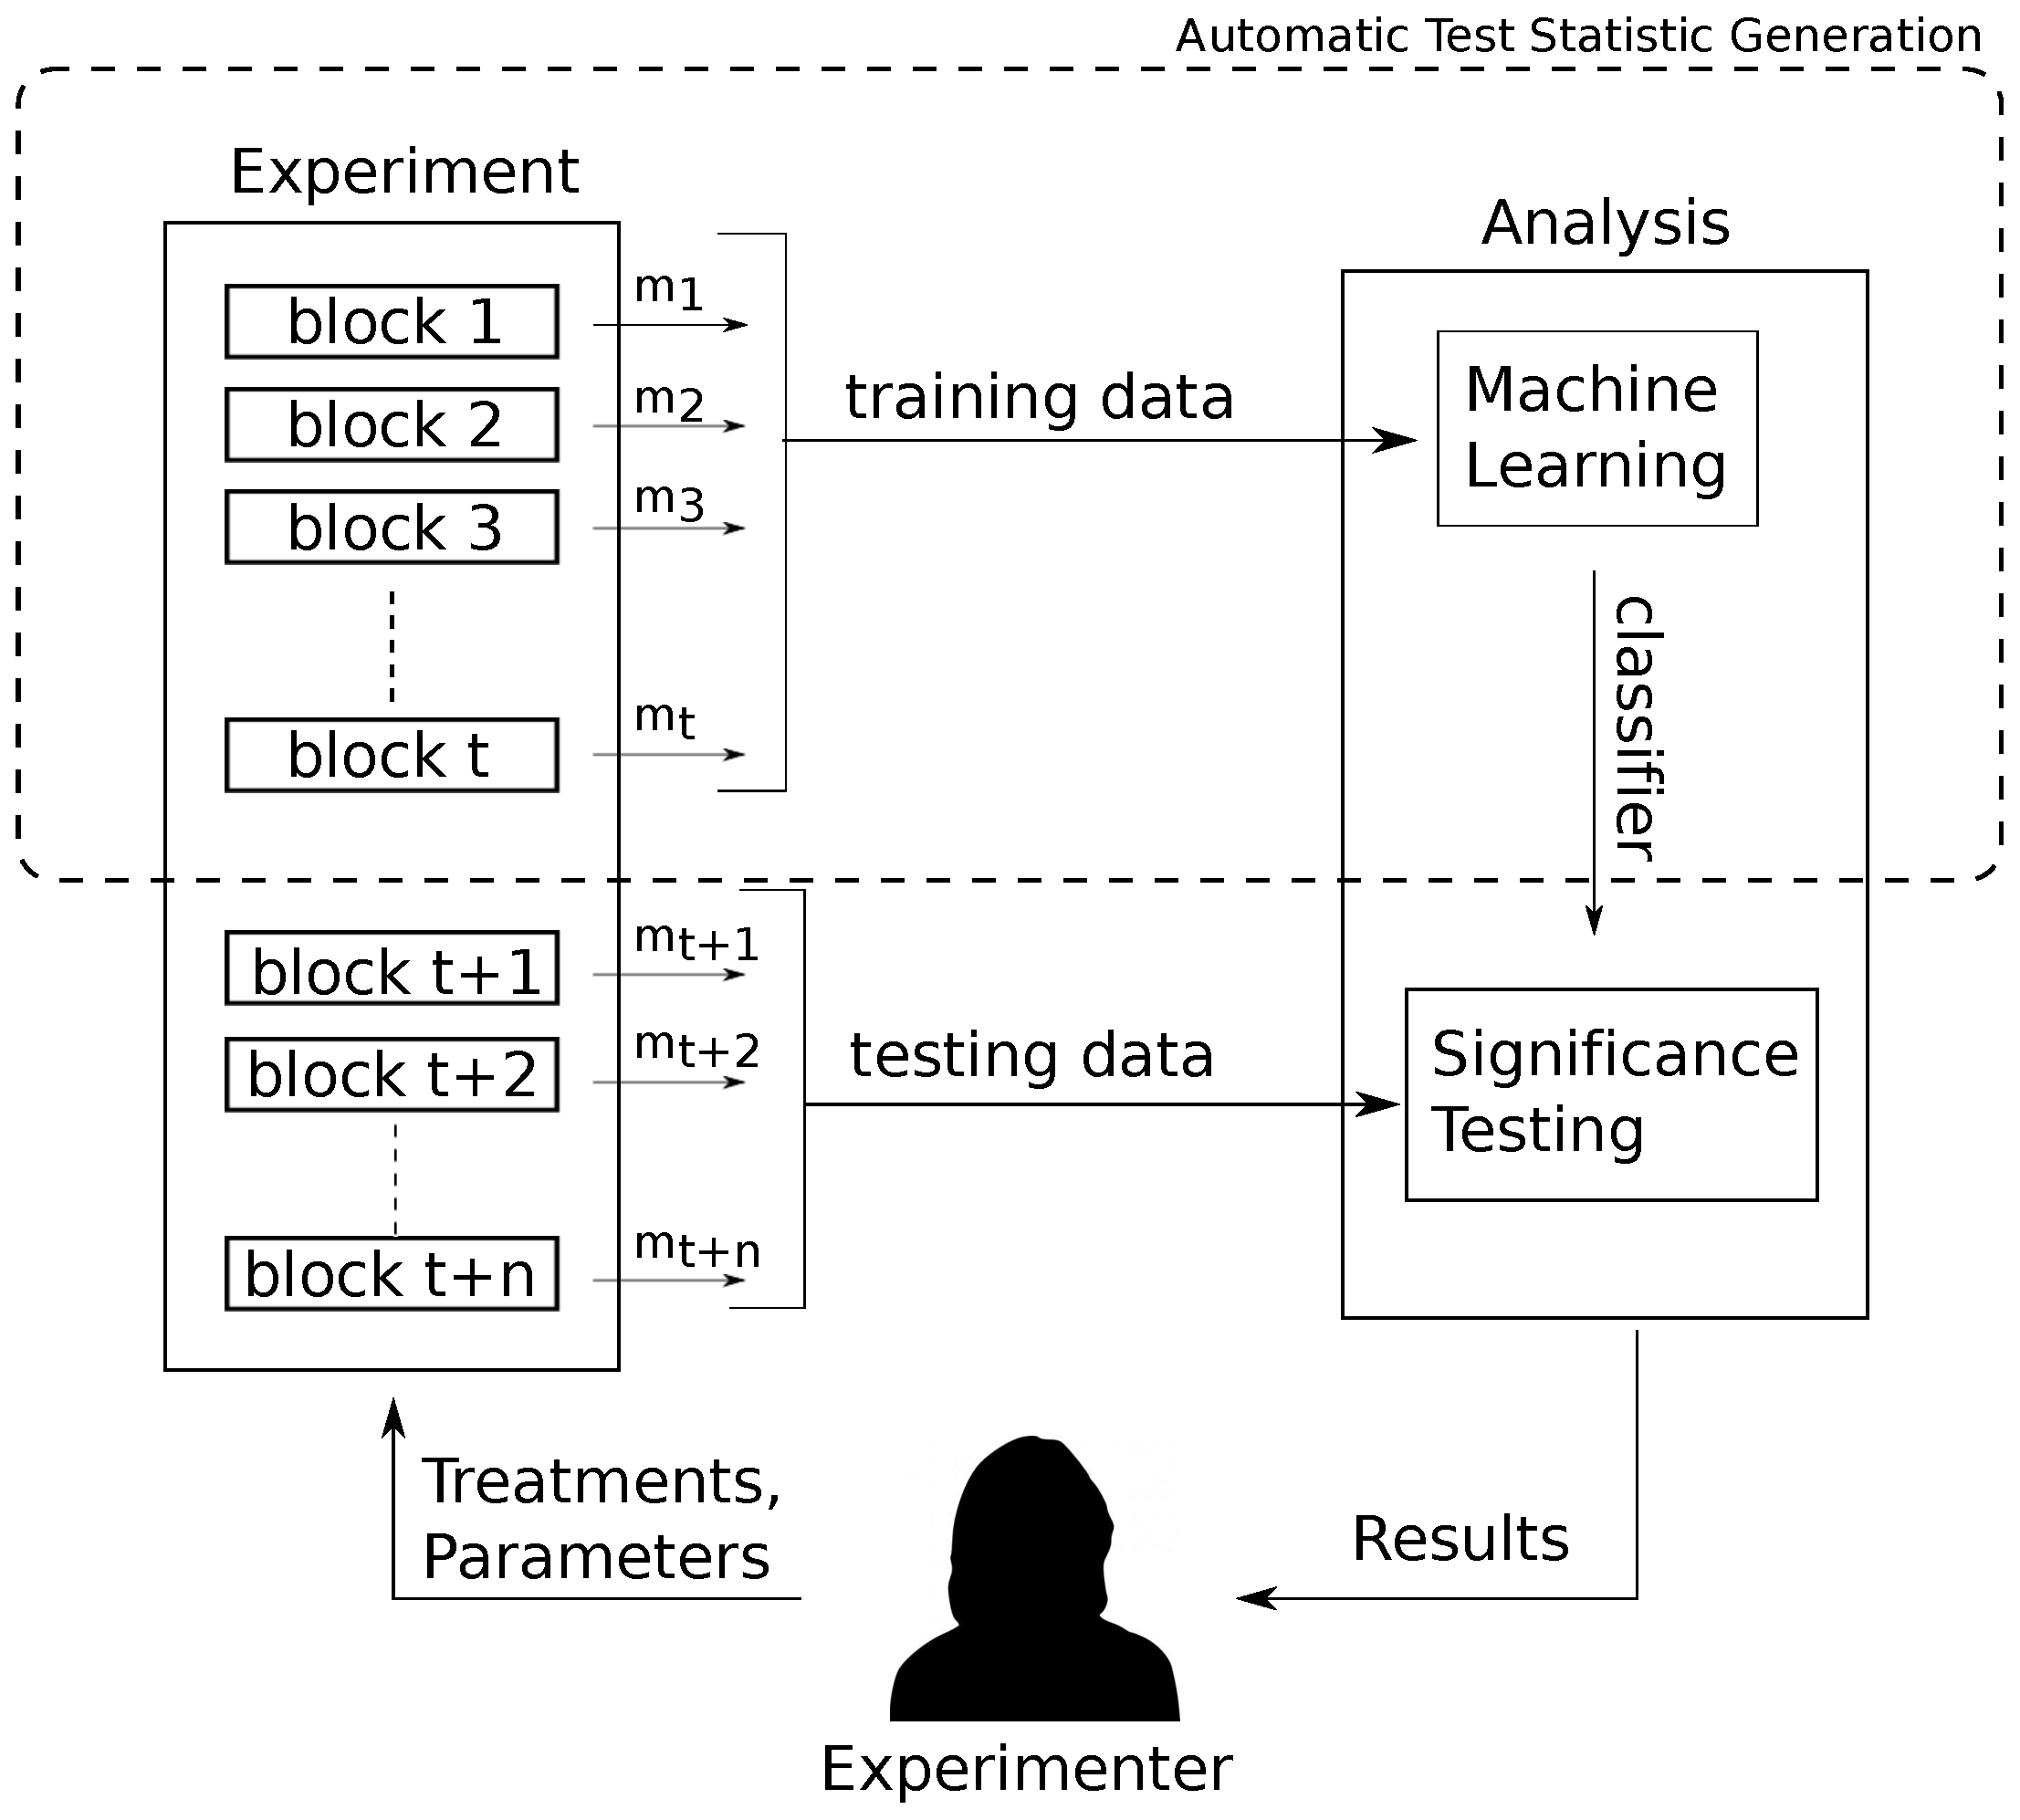
\includegraphics[width = 7cm]{images/methodology2.eps}
\end{center}
\caption{Our experimental setup with training and testing blocks. Measurements from the training blocks are used to build a classifier. The trained classifier is used to compute the test statistic on the measurements from the testing blocks for significance testing.}\label{fig:meth2}
\end{figure}
%\begin{figure}
%\begin{center}
%\includegraphics[width = 8cm]{workflow.eps}
%\end{center}
%\caption{Figure depicting the structure of our experiment.}
%\label{fig:workflow-final}
%\end{figure}

We partition the collected data into training and testing subsets, 
and use the training data to train a classifier. 
We perform $10$-fold cross validation on the training data
to select appropriate parameters. The classifier is trained to predict which treatment a 
browser instance received, only from the ads that get served to that instance. 
If the classifier is able to make this prediction with high accuracy, 
it suggests a systematic difference between the ads served to the 
two groups that the classifier was able to learn. 
If no difference exists, then we would expect the number to be near 
the guessing rate of $50\%$. AdFisher uses the accuracy of this 
classifier as its test statistic. 

%To avoid the possibility of seeing a high accuracy due to overfitting, 
AdFisher evaluates the accuracy of the classifier on a testing data set 
that is disjoint from the training data set.  
%That is, in the language of statistics, 
%we form our hypothesis about the test statistic being able to distinguish 
%the groups before seeing the data on which we test it to ensure that it 
%has predictive power. 
AdFisher uses the permutation test to determine 
whether the degree to which the classifier's accuracy on the test data 
surpasses the guessing rate is statistically significant.  That is, it calculates 
the p-value that measures the probability of seeing the observed accuracy 
given that the classifier is just guessing.  If the p-value is below $0.05$, 
we conclude that it is unlikely that classifier is guessing and that it must 
be making use of some difference between the ads shown to the two groups.

\subsubsection{Explanations}%\label{sec:MLfeatsel}
To explain how the learned classifier distinguished between the groups, 
we tried out several methods. 
We explored using simple metrics for providing explanations, like ads 
with the highest frequency in each group. However, some generic ads 
gets served in huge numbers to both groups. We also looked at the 
proportion of times an ad was served to agents in one group to the total 
number of times observed by all groups.  However, this did not provide 
much insight since the proportion typically reached its maximum value of 
$1.0$ from ads that only appeared once. 

We found the most informative explanation to be the model produced 
by the classifier itself. 
We used a linear classifier (logistic regression) to select our test statistic.
Recall that logistic regression weighs the various features of the instances 
with coefficients reflecting how predictive they are of each group.  
Thus, examining the ads with the most extreme coefficients identifies 
the ad pair most used to predict the group to which agents receiving 
that ad belongs.

%in a decision function whose value predicted the group of the instance.  Coefficients of large positive value imply that that feature is associated with being of the first group; negative values are associated with the second group; values near zero are uninformative.
%
%To measure how informative a subset of features is, AdFisher is able to find the features with the most positive coefficients and those with the most negative coefficients.  With them, AdFisher can perform model selection and fitting again while using just these features to obtain the testing accuracy of a new model using the reduced subset of features.  If this model is also accurate, then it shows that these features alone are able to distinguish between the groups.
%Refer to Table~\ref{tab:gen+jobs-featsel} for the results of this analysis on the data generated in Experiment~\ref{exp:gen+jobs}.
%We also computed the two count based metrics we described above for each of the $10$ features selected from the Machine Learning algorithms for comparison. Note that


%Another choice we explored was to compute the difference in the number of times an ad appears between the groups.  However, this metric is also highly influenced by how common the ad is across all groups.  %Thus, we take the difference divided by the total number of times the ad shows up to measure the


%For further justification of using permutation tests to infer causation, see~\cite{greenland11book}.  For computational reasons, sampling is often used to approximately solve for $\pt(s,\vec{y})$

%Permutation testing is not without assumptions.  First, the experimental units must start out exchangeable: we must not have any reason to believe that any one is more likely than the others to show any of he possible resposes.  Second, at least in its basic form, the units must be randomly assigned a treatment making these tests inapplicable to observational studies (e.g., surveys) in which the scientist cannot control the treatment.  Third, the units must be independent in the sense that treating one does not affect others as discussed in Section~\ref{sec:doe}.  Lastly, the test relies on a frequentist interpretation of statistics making its status questionable at best to those who only accept Bayesian methods~\cite{xxx}.

%A limition is that computing the value of $\pt(s, \vec{y})$ is made difficult by the number of permutations increasing rapidly with the sample size.  Two techniques are typically used.  The first is to approximate its value by sampling.  The second is to exploit symmetries in the test statistic that make some permutations redundant.  For example, the differences of means test statistic does not depend upon the order of the first $n$ or $m$ components and could be treated as a function on two sets.  Thus, it is expressible as $s'(G_1,G_2)$ and we can consider the space of all partitions of a fixed size rather than the space of all permutations.  

% We do not claim that permutation tests are the only suitable statistical tests.  However, we find it sufficient to characterize the prior WDUD works, which we do next.


% \begin{figure}
% \begin{center}
% \includegraphics[width = 8cm]{block3.eps}
% \end{center}
% \caption{Experimental setup to carry out significance testing on $8$ browser agents comparing the effects of two treatments. Each agent produces performs actions on the web and produces measurements}
% \label{fig:block}
% \end{figure}


%\subsubsection{Discussion}
%
%
%%\subsection{Avoiding Pitfalls}
%%\paragraph{Avoiding Pitfalls}
%The above method avoids some pitfalls.
%Most fundamentally, we use a statistical analysis whose assumptions matches those of our experimental design.
%Assumptions required by many statistical analyses appear unjustifiable in our setting.  
%% For example, many analyses assume that the agents do not interact or that the ads are independent and identically distributed (e.g.,~\cite{barford14www}).  
%% However, given that all the agents receive ads from the same pool of possible ads governed by the same advertisers' budgets, these assumptions appear unlikely to hold.
%% Indeed, empirical evidence suggests that it does not~\cite{tschantz14arxiv}.
%% Our use of the permutation test, which does not require this assumption, allows us to ensure the statistical soundness of our analysis without making these assumptions~\cite{greenland86epidemiology}.
%
%%By reporting a p-value, we provide a quantitative measure of the confidence we have that the observed effect is genuine and not just by chance~\cite{jensen92phd}.
%%
%\begin{remark}
%The permutation test provides a method of determining whether a system has interference that is probabilistically sound to a degree quantified by the p-value.
%\end{remark}
%
%Our use of randomization implies that many factors that could be confounding factors in an unrandomized design become noise in our design (e.g.,~\cite{good05book}).  While such noise may require us to use a large sample size to find an effect, it does not affect the soundness of our analysis.
%We expect our methodology to suggest that an effect exists when one does not with a probability equal to or less than the p-value. 
%
%
%
%%Relatedly, 
%%Reporting simply the classifier accuracy or that some difference occurred fails to quantify the possibility that the result was a fluke.
%%\paragraph{Limitations}
%%\subsection{Scope}
%%\label{sec:scope}
%% We restrict the scope of our methodology to making claims that an effect exists with high likelihood as quantified by the p-value.
%% That is, 
%
%%We only claim statistical soundness in the sense that upon reporting that a treatment causes an effect, such an effect really was caused by the treatment with high likelihood (made quantitative by a p-value).
%%While we provide rigor in the area of drawing sound statistical conclusions, our method does have two important limitations.  First,
%
%\begin{remark}
%The permutation test is not sound for finding noninterference nor complete for finding interference.
%\end{remark}
%
%%We do not claim the converse, that is, ``completeness'' or ``power'': 
%Our method might fail to detect some use of information.  For example, the web service's behavior might vary by some feature not measured by the test statistic.
%
%Furthermore, we do not claim that results generalize beyond the setting of the experiment.  To do so, our method may be combined with random sampling and methods to ensure that the observed system does not attempt to evade the study.
%
%%we would need to a take a random sample of all users, their IP addresses, browsers, and behaviors, which is prohibitively expensive.  For example, instead of turning off some usage upon detecting our tool, Google might turn it on.  While the detected usage would be real (and our method sound), it might not be experienced by normal users.  However, it would be odd if Google purposefully performs questionable behaviors only in front of those attempting to find it.
%
%Lastly, we do not claim that our method shows how the system in question uses information internally.  
%Any observed effect may be the result of complex interactions between the system and other ones in its environment.
%In particular, as discussed in Section~\ref{sec:ife-impossible}, our method finds interference not within the system in isolation, 
%but rather for the system operating in its environment.


% It could have been used by Google directly for targeting or it could have been used by advertisers to place their bids.  We cannot assign blame.  
%We hope future work will shed light on these issues, but given that we cannot observe the interactions between Google and advertisers, we are unsure whether it can be done.

%\subsection{Discussion}

\section{Analyzing Google's ad ecosystem}

We first provide a brief description of Google's ad ecosystem and then discuss
discuss experiments to study the
three privacy and fairness properties: discrimination, transparency and choice.


\subsection{Google's ad ecosystem}

The advertising ecosystem is a vast decentralized system 
with several actors including the online consumers, the advertisers, the publishers 
of web content, and ad networks.  Websites publishing content 
integrate ads served by ad networks, such as Google, into their 
content by providing empty slots on their webpages 
into which standard-sized ads fit.  Advertisers provide ads designed to fit 
these slots to ad networks. When an individual visits a 
publisher's webpage, the ad network determines which ad to place in the 
available slots of that webpage.  To make this determination, ad networks 
use proprietary algorithms that among other variables take into account 
the expressed preferences of advertisers and publishers, and if ads are 
behaviorally targeted the specific user's behavior and, if communicated, preferences.  

Users have some say over the advertisements Google serves them. 
Ad Settings is a Google tool that helps users control the ads they see on 
Google services and on websites that partner with 
Google. It allows users to independently 
select attributes for ad-targeting and enables them to see and modify 
ad-targeting inferences that Google has made about the user. Ad Settings 
attributes include both demographics and interests based on browsing behavior.
Users can view and edit these settings at \url{www.google.com/settings/ads}.
%Yahoo~\autocite{yahoo-help}
%and Microsoft~\autocite{microsoft-choice} offer similar tools for personalizing ad settings.

Google's Ad Settings, and similar functionality provided by other 
advertising platforms, respond to regulators' and users' concerns 
about behavioral marketing on the web. %~\autocite{ur12soups}.  
They provide some transparency about how users are sliced and diced for 
ad-targeting, and allow users to exercise some modicum of control over 
the ads they see, including the ability to limit ads from Google 
targeted based on previous web activity and 
demographic details . 
%For example, Google provides individuals with the 
%ability to limit ads based on ``your interests, previous visits to other websites, 
%and demographic details on your computer's browser'' served on their properties 
%and by their advertising network.~\footnote{\url{https://support.google.com/ads/answer/2662922?hl=en}}

%The ad ecosystem 
%consists of several players including the advertisers, the publishers, and the users. 
% and serves personalized ads to users.
%These algorithms operate on inputs from
%all the various players in the ad ecosystem, like the advertisers, the publishers, and
%the users. 
%By considering users' past behavior and ads' past performance, 
%the system personalizes ads for users. 
%To provide some insight and control over ads, Google 
%provides Ad Settings,\footnote{\url{www.google.com/settings/ads}}
%a transparency and choice tool where users can view and edit
%inferences made by the system. 
%We use AdFisher to analyze ads served by Google 
%and the information provided on Ad Settings
%to study three properties - discrimination, opacity (a lack of transparency), 
%and choice. We encode these properties in terms of information 
%flows through the system. By detecting certain flows of information, we find compliance
%or violations of these properties~\cite{datta2015automated}. 
%%These decisions are some
%%of the most ubiquitous automated algorithmic decisions that we encounter.
%%We applied our IFE methodology to study 
%%While ads are not always as crucial as some of the other decisions, given their 
%%abundance, they are an appropriate target to study the effect of algorithmic 
%%decisions. 
%%Another subject of our analysis was Google's transparency and choice tool, 
%%Ad Settings, 
%%for our experiments. This tool is for customers to view what
%%Google has inferred about them (transparency), as well as make edits
%%to those inferences (choice). In our experiments, we used the tool to relay  
%%information (e.g. gender), as well as for measuring inferences made. 
%
%To study an instance of discrimination, we search for a flow of 
%information from gender to ads in the context of job-searching behavior. 
%We set up AdFisher to have units in one group set gender to 
%female on Ad Settings, while units in the other group set 
%theirs to male. To simulate job-seeking behavior, all units 
%visit the top hundred websites for employment on  
%Alexa top sites\footnote{\url{alexa.com/topsites/category/Top/Business/Employment}}. From the experiment, we find a causal effect of gender on the 
%ads served by Google on third-party news websites. How the ads differ is 
%concerning as well. The top two ads served to male units are for a 
%career coaching service for $\$200$k+ executive positions. 
%The male units received the ads $1852$ times, whereas the female units only 
%$318$ times.
%On the other hand, the top two ads for the female group are for a generic job posting 
%service and for an auto dealer. This experiment demonstrates that Google may serve 
%job-related ads to male and female job-seekers disparately.
%% \amit{fix}
%
%%AdFisher ran the experiment with $1000$ browser instances. 
%%It used ads of $900$ agents ($450$ from each group) for training a classifier 
%%using the URL+title feature set, and used the remaining $100$ agents' ads for testing.  
%%To test whether this response was statistically significant, 
%%AdFisher computed a p-value by running the permutation test on a 
%%million randomly selected permutations of the data.
%%The significance test yielded an adjusted p-value of $< 0.00005$. %0.0000424}.
%%We then examined the model learned by AdFisher to explain the nature of the difference.
%
%To detect opacity, we seek a flow from online activities
%to ads served, in the absence of a flow to Ad Settings. 
%This would indicate that a flow from online actions to ads is not reflected on the 
%transparency tool, thereby demonstrating opacity. 
%We set up AdFisher to drive the experimental units
%to visit the top hundred websites on substance abuse, while the control units
%do not visit any. We observe a causal effect on the ads, where an alcohol
%and drug rehabilitation center ad (\url{thewatershed.com}) is served in large numbers 
%and exclusively to the experimental units. The causal effect demonstrates a flow from 
%the website visits to the ads. However, we find no change in 
%the information displayed on the Ad Settings page, thereby indicating that there 
%is no flow to Ad Settings. This is an instance where the transparency tool 
%	is being opaque to users.
%
%Finally, we analyze whether Ad Settings respects  
%user choice, where we are interested to see if making changes on  
%Ad Settings affects ads as expected. We observe that `opting out
%of behavioral ads' causally affects the ads. When both groups of browser units
%visit car-related websites, the top ads for units that opt out are not car related, 
%while those for other units are. In another experiment, we observe that 
%removing an interest for dating reduces the number
%of dating related ads being served. Thus, Ad Settings appear to respect 
%user choice.
%
%These findings received a lot of public attention and caused quite a media 
%stir.\footnote{For a list of press articles and more details about our results, 
%please visit \url{possibility.cylab.cmu.edu/adfisher/}}
%%Google added a footnote on Ad Settings 
%Shortly after publication of our results, Google updated Ad Settings to require signing in to
%an account for access. This made further evaluation of Google's systems difficult. 
%Nevertheless, these investigations demonstrate the utility of the IFE methodology and 
%are the first to apply causal methods to discover discrimination, opacity, 
%and respect for choice on the Google ad ecosystem. 
%%Nevertheless, our results were the first to provide a starting point for deeper analysis from the inside.

%\subsection{AdFisher}

%With the advancement of tracking technologies and the growth of online data aggregators, data collection on the Internet has become a serious privacy concern. Colossal amounts of collected data are used, sold, and resold for serving targeted content, notably advertisements, on websites
%%Online advertisers target ads to Internet users based on their browsing behaviors 
%(e.g.,~\cite{mayer12sp}).  Many websites providing content, such as news, outsource their advertising operations to large third-party ad networks, such as Google's DoubleClick.  These networks embed tracking code into webpages across many sites providing the network with a more global view of each user's behaviors. 
%
%People are concerned about behavioral marketing on the web~(e.g.,~\cite{ur12soups}). %They are often unaware of what data companies use to determine the ads they show to them. %They would like to know what information companies use to determine the ads they show to them.
%%Google has provided the Ad Settings webpage that allows users to view various information about how Google categorizes their behavior.  However, questions remain about how it operates.
%To increase transparency and control, %into these issues, 
%Google provides Ad Settings, which is ``a Google tool that helps you control the ads you see on Google services and on websites that partner with Google''~\cite{google-ad-settings-help}. It displays inferences Google has made about a user's demographics and interests based on his browsing behavior.
%%is dynamically generated for each user (as approximated with tracking cookies).  
%Users can view and edit these settings at\\
%\centerline{\url{http://www.google.com/settings/ads}} %  Google defines it as 
%%A user can also edit these demographics.
%%Figure~\ref{fig:settings} provides a screenshot.
%%\begin{figure}
%%\begin{center}
%%\includegraphics[width=8cm]{images/settings-short.eps}
%%\end{center}
%%\caption{Screenshot of Google's Ad Settings webpage}
%%\label{fig:settings}
%%\end{figure}
%Yahoo~\cite{yahoo-help}
%and Microsoft~\cite{microsoft-choice} also offer personalized ad settings.
%
%However, they provide little information about how these pages operate, leaving open the question of
%%leaving the operation of these transparency mechanisms rather opaque.
%%We would like to know 
%how completely these settings describe the profile they have about a user. In this study, we explore how a user's behaviors, either directly with the settings or with content providers, alter the ads and settings shown to the user and whether these changes are in harmony. 
%% We also look into how changing settings affect ads. 
%In particular, we study the degree to which the settings provides transparency and choice as well as checking for the presence of discrimination.
%Transparency is important for people to understand how the use of data about them affects the ads they see.
%Choice allows users to control how this data gets used, enabling them to protect the information they find sensitive.
%Discrimination is an increasing concern about machine learning systems and one reason people like to keep information private~\cite{bigdata14whitehouse, zemel13icml}.

%%% AMIT WROTE
%To observe how ads served to two groups of individuals differing on some sensitive attribute differ, we run experiments where automated browser agents simulating users interact with Google and content providers.  We simulate individuals by visiting websites and altering ad settings, and observe how they affect the ads that Google shows.} %, as a result of which there are growing demands for transparency into their workings.}

%We also look into how changing settings affect ads. 
%By running experiments where automated browser agents simulating users interact with Google and content providers, we measure how these interactions alter the ads and settings that Google shows.



%\paragraph{Overview of Apporach}
%To conduct these studies, we developed AdFisher, a tool for automating randomized, controlled experiments for studying online tracking.
%Our tool offers a combination of automation, statistical rigor, scalability, and explanation for determining the use of information by web advertising algorithms and by personalized ad settings, such as Google Ad Settings.
%The tool can simulate having a particular interest or attribute by visiting webpages associated with that interest or by altering the ad settings provided by Google.  It collects ads served by Google and also the settings that Google provides to the simulated users. It automatically analyzes the data to determine whether statistically significant differences between groups of agents exist.  AdFisher uses machine learning to automatically detect differences and then executes a test of significance specialized for the difference it found.


%It experiments with \emph{agents}, automated browser instances that simulate users by visiting and interacting with webpages.
%The tool randomly assigns various agents to either control or experimental groups.
%Each group receives a different \emph{treatment}, a script of behaviors that the agents perform to possibly establish some profile with Google.
%The tool then makes the same measurements of the agents across the two groups to determine whether the groups differ under that measurement.
%For example, the tool can measure the ads that an agent receives upon visiting a particular webpage or the agent's Ad Settings.
%
%Lastly, the tool runs an automated analysis to test for statistically significant differences between the groups of agents.
%In particular, the tool attempts to reject the null hypothesis that differences between the two treatments had no effect upon the measurements taken.  If the tool can reject the null hypothesis, then it has statistically established the use of information about the differences between the groups.
%
%To keep the analysis automated, the tool uses machine learning to select the statistical analysis to use.
%In particular, it selects a classifier that attempts to determine from the measurements made for each agent to which group the agent belongs.
%An accurate classifier corresponds to finding a difference between the groups.
%To avoid finding differences just by chance (analogous to \emph{overfitting} in machine learning or \emph{data dredging} in statistics), the tool selects the classifier training data that is separate from the test data used for the statistical analysis.
%We provide functions making the specification of the treatments and measurements used in our experiments easy.
%The tool also analyzes the classifier to characterize the differences between the groups.

%Someone using AdFisher to study behavioral targeting only has to provide the behaviors the two groups are to perform (e.g., visiting websites) and the measurements (e.g., which ads) to collect afterwards. 
%% they perform those behaviors. 
%AdFisher can easily run multiple experiments exploring the causal connections between users' browsing activities, and the ads and settings that Google shows.
%
%The advertising ecosystem is a vast, distributed, and decentralized system with several players including the users consuming content, the advertisers, the publishers of web content, and ad networks.  With the exception of the user, we treat the entire ecosystem as a blackbox.  We measure simulated users' interactions with this blackbox including page views, ads, and ad settings.  
%Without knowledge of the internal workings of the ecosystem, we cannot assign responsibility for our findings to any single player within it nor rule out that they are unintended consequences of interactions between players.
%However, our results show the presence of concerning effects illustrating the existence of issues that could be investigated more deeply by either the players themselves or by regulatory bodies with the power to see the internal dynamics of the ecosystem.


\subsection{Experimental Results}

We perform a total of
$21$ experiments to study properties of discrimination, transparency and choice
on Google's ad ecosystem. Table~\ref{tbl:results} presents a summary of 
all our experiments. 

\begin{table*}
\begin{tabular}{llL{1.5cm}llL{1cm}rl}
\hline
Property & Treatment & Other Actions & Source & When & Length (hrs) & \# ads & Result \\
\hline
Nondiscrimination %&  && Violation\\
& Gender & - & TOI & May & $10$ & $40,400$ & Inconclusive\\
& Gender & Jobs & TOI & May &  $45$ & $43,393$ & Violation\\
& Gender & Jobs & TOI & July & $39$  & $35,032$ & Inconclusive\\
& Gender & Jobs & GDN & July & $53$ & $22,596$ & Inconclusive\\
& Gender & Jobs \& Top 10 & TOI & July & $58$ & $28,738$ & Inconclusive\\
\hline
%Individual 
Transparency %& && Violation\\
& Substance abuse & - & TOI & May & $37$ & $42,624$ & Violation\\
& Substance abuse & - & TOI & July & $41$ & $34,408$  & Violation\\
& Substance abuse & - & GDN & July & $51$ & $19,848$   & Violation\\
& Substance abuse & Top 10 & TOI & July & $54$ & $32,541$   & Violation\\
& Disability & - & TOI & May & $44$ & $43,136$   & Violation\\
& Mental disorder & - & TOI & May & $35$ & $44,560$  & Inconclusive\\
& Infertility & - & TOI & May & $42$ & $44,982$  & Inconclusive\\
& Adult websites & - & TOI & May & $57$ & $35,430$  & Inconclusive\\
\hline
Effectful choice  %& && Compliance\\
& Opting out & - & TOI & May & $9$ & $18,085$  & Compliance\\
& Dating interest & - & TOI & May & $12$ & $35,737$  &  Compliance\\
& Dating interest & - & TOI & July & $17$ & $22,913$  &  Inconclusive\\
& Weight loss interest & - & TOI & May & 15 & $31,275$  &  Compliance\\
& Weight loss interest & - & TOI & July & 15 & $27,238$  &  Inconclusive\\
\hline
Ad choice 
& Dating interest  & - & TOI & July & 1 & $1,946$   &  Compliance\\
%& Weight loss interest & ``fitness'' & Inconclusive\\
%& Weight loss interest & many keywords & Inconclusive\\
& Weight loss interest  & - & TOI & July & 1 & $2,862$   &  Inconclusive\\
& Weight loss interest  & - & TOI & July & 1 & $3,281$   &   Inconclusive\\
\hline
\end{tabular}
\caption{%
Summary of our experimental results. % Testing Privacy Properties. 
% For each property, we ran experiments exploring different interests and demographics. 
% Additional actions are performed by both the experimental and control agents. 
Ads are collected from the Times of India (TOI) or the Guardian (GDN), 
either in May or July $2014$. 
% For each experiment, we show how long it took, the number of ads collected, and result.
% We show how long each experiment took and how many ads we collected for that experiment. 
% The final column reports our finding from the experiment.
We report how long each experiment took, how many ads were collected for it, and what result we concluded.
}
\label{tbl:results}
\end{table*}

\subsubsection{Discrimination}

%We also found evidence suggestive of \emph{discrimination} from another experiment.
%We set the agents' gender to female or male on Google's Ad Settings page.  We then had both the female and male groups of agents visit webpages associated with employment.  %Again using the ads on the Times of India, w
%We established that Google used this gender information to select ads, as one might expect. The interesting result was how the ads differed between the groups: during this experiment, Google showed the simulated males %certain 
%ads from a certain career coaching agency that promised large salaries more frequently than the simulated females, a finding suggestive of discrimination. 
%Ours is the first study that provides statistically significant evidence of an instance of discrimination in online advertising when demographic information is supplied via a transparency-control mechanism (i.e., the Ad Settings page).
%% \mct{Make clear that we're only talking about a single class of ad; not wide spread discrimination.}
% Furthermore, while our finding of discrimination in the non-normative sense of the word is on firm statistical footing, we acknowledge that people may disagree about whether we found discrimination in the normative sense of the word.  We defer discussion of whether our findings suggest unjust discrimination until Section~\ref{sec:disc}.


We use AdFisher to demonstrate a violation in the nondiscrimination property. %can demonstrate discrimination.
If AdFisher finds a flow of information from a protected attribute to 
the ads served, then we have evidence that Google's ad ecosystem discriminates
on that attribute. 
% significant difference in how Google treats 
%two experimental groups, one consisting of members having a protected 
%attribute and one whose members do not, then the experimenter has strong 
%evidence that Google discriminates on that attribute.
%In particular, we use AdFisher's ability to automatically select a test statistic to check for possible differences to test the null hypothesis that the two experimental groups have no differences in the ads they receive.
%A limitation is that experiments cannot prove the absence of discrimination since they cannot prove the absence of an effect (see Section~\ref{sec:scope}).
As mentioned before, it is difficult to send a clear signal about any attribute by 
visiting related webpages since they may have content related to other attributes. 
The only way to send a clear signal is via Ad Settings. 
Thus, we focus on attributes that can be set on the Ad Settings page.  
% In particular, we explored whether Google's reactions were appropriate.  
In a series of experiments, we show how gender information on Ad Settings flows to
ads served. 
%We detect this flow of information by randomly setting different genders
%on different agents. 
%of one group to female and the other to male.  
%In one of the experiments, the agents went straight to collecting ads; in the others, they simulated an interest in jobs.  %In another two experiments, we set the age either to be $18$--$24$ or to be $65+$ with one experiment simulating an interest in jobs.I
%We found a statistically significant difference in the ads for male 
%and female agents that simulated an interest in jobs.
%We also found evidence of discrimination in the nature of the effect.  
%In particular, 
%% in the gender and jobs experiment, we 
%we observed that females received fewer instances of an ad encouraging the taking of high paying jobs than males.  
%%AdFisher did not find any statistically significant differences among the agents that did not visit the job-related pages or those operating in July, 2014.
%%AdFisher did find a statistically significant effect for the agents that did visit the job-related sites as one would expect.
%%  However, in one experiment, we also found evidence of discrimination in the nature of the effect.  In particular, in the gender and jobs experiment, we found females received fewer ads encouraging the taking of high paying jobs than males.  
We detail one experiment which found evidence of discrimination.
%We detail one of these experiments below.

%
%\paragraph{Gender and Jobs}
%In this experiment, we examine how changing the gender demographic on Google Ad Settings affects the ads served and interests inferred for agents browsing employment related websites.
We set up AdFisher to have the browser instances in one group visit the Google Ad Settings 
page and set the gender bit to female while agents in the other group set theirs to male.
All the instances then visited the top hundred websites related to employment
and then collect ads from Times of India.
AdFisher ran the experiment in $100$ blocks of $10$ instances each. 
AdFisher used the ads of $900$ instances ($450$ from each group) for 
training a classifier %using the URL+title feature set, 
and used the remaining $100$ instances' ads for testing.  
The learned classifier attained a test-accuracy of $93\%$, 
suggesting that Google did in fact treat the genders differently.
To test whether this response was statistically significant, 
AdFisher computed a p-value by running the permutation test, which
yielded an adjusted p-value of $< 0.00005$. %0.0000424}.

%Setting the gender bit did have a significant effect on the ads shown.
%AdFisher found a classifier with a test-accuracy of $93\%$.
%The p-value was $5.298*10^{-6}$.
%The only difference between the two treatments was gender bit on Google Ad Settings. The results from the analysis are presented in Table~\ref{tab:res}. A p-value of XX means that the treatment had a significant effect on the ads. 
%We then examined the model learned by AdFisher to explain the nature of the difference.
%We looked at the URL+title pairs with the highest coefficients for identifying each gender's  group.
%To explain this difference, we look at the learned model.
%Table~\ref{tab:gen+jobs-featsel} shows the five URL+title pairs that the model identifies as the strongest indicators of being from the female or male group.
How ads for identifying the two genders differ is also concerning from a discriminatory
standpoint. The two ads with the highest coefficients for indicating a 
male were for a career coaching service for ``$\$200$k+'' executive positions. 
Google showed the ads $1852$ times to the male group 
but just $318$ times to the female group.
The top two ads for the female group were for a generic job posting service 
and for an auto dealer.

% We believe these results suggest the possibility of discrimination, intentional or otherwise.  
% Google or the advertiser might have purposely targeted just males.
% Alternatively, males might be more likely to click on an ad for a high-paying job than females, and Google may have picked up this signal from past interactions with other users.
% %Another interesting ad is the one about `Transport Trucking' which is the fifth top ad for the {\em male} treatment. 
% %But this seems unfair, just like its unfair to not interview women for a traditionally male dominated high-paying job.
% Google's policies allow it to serve different ads based on gender, but dissimilarities of this kind are concerning even if unintentional and allowed.  \nnnew{We discuss this issue more in Section~\ref{sec:disc}.}
 

%%\smallskip
%The found discrimination in this experiment was predominately from a 
%pair of job-related ads for the same service making the finding highly 
%sensitive to changes in the serving of these ads.
%A closer examination of the ads from the same experimental setup 
%ran in July, 2014, showed that the frequency of these ads reduced 
%from $2170$ to just $48$, with one of the ads completely disappearing.
%These $48$ ads were only shown to males, continuing the pattern of discrimination.
%This pattern was recognized by the machine learning algorithm, 
%which selected the ad as the second most useful for identifying males.  
%However, they were too infrequent to establish statistical significance.
%A longer running experiment with more blocks might have succeeded.


%, prehabes reflecting a change in the adversiers budget or stragety, or a change in Google's selection of the ad.
%The $48$ ads that were shown \mct{here}
% we believe that visiting the job-related websites is necessary to meet the ads' targeting criteria.  
%We further believe that the absence of discrimination in July steams from the budget of those ads being decreased when we tested in July.  Whereas they appeared $2170$ times in the significant experiment in May, they only appeared $48$ times to the same experimental setup in July.  
%While all $XX$ \mct{??} were to male agents, the small number of occurrences were not sufficient for AdFisher to find the discrimination.
%\mct{add hand crafted permutation test showing that ML is to blame?}

%\begin{experiment}\label{exp:subs}

\subsubsection{Opacity}

%In one experiment, we explored whether visiting websites related to substance abuse has an impact on Google's ads or settings.  We created an experimental group and a control group of agents.  The browser agents in the experimental group visited  websites on substance abuse while the agents in the control group simply waited.  Then, both groups of agents collected ads served by Google on a news website. % - the Times of India. %, a content providing webpage that uses Google for advertising.  We collected the ads shown to the agents.  %We also collected
%
%Having run the experiment and collected the data, we had to determine whether any difference existed in the outputs shown to the agents.  One way would be to intuit what the difference could be (e.g. more ads containing the word ``alcohol'') and test for that difference.  %For example, we might have suspected that the experimental group would have received %more ads containing the word ``alcohol''.  
%%Thus, we could use the \emph{test statistic} that counts the number of instances of ``alcohol'' in the ads of the experimental group and subtracts from it the number of times it appears in the control group. 
%% If no difference exists, we would expect this test statistic would have a value close to zero.  If our suspicion is correct, we would expect a large positive value.
%However, developing this intuition %the intuition that ``alcohol'' is a difference between the groups 
%can take considerable effort. Moreover, it does not help find unexpected differences. Thus, we instead used
%%AdFisher uses 
%machine learning to automatically find differentiating patterns in %a training subset of 
%the data. Specifically, AdFisher finds a classifier that can predict which group an agent belonged to, from the ads shown to an agent. %, accurately determine whether the agent visited the webpages related to substance abuse.  
%The classifier is trained on a subset of the data. A separate test subset is used to determine whether the classifier found a statistically significant difference between the ads shown to each group of agents.
%In this experiment, AdFisher found a classifier that could distinguish between the two groups of agents by using the fact that only the agents that visited the substance abuse websites received ads for Watershed Rehab.
%
%We also measured the settings that Google provided to each agent on its Ad Settings page after the experimental group of agents visited the webpages associated with substance abuse.  We found no differences (significant or otherwise) between the pages for the agents.  Thus, information about visits to these websites is indeed being used to serve ads, but the Ad Settings page does not reflect this use in this case. % Thus, we conclude that the settings provided by Google do not provide a complete picture of what is being or may be used to serve ads.  %Thus, we conclude that Google is using information related to visiting webpages associated with substance abuse but not reporting this use.  
%Rather than providing transparency, in this instance, the ad settings were \emph{opaque} as to the impact of this factor.

%We ran a similar experiment using webpages related to disabilities.  This time we found statistically significant changes to both the ads and the settings.  However, only the changes to the ads appear related to the disabilities.


%Our findings relate are of the vastly complex and decentralized ad ecosystem (comprising of the advertisers, consumers, publishers, etc.), and we cannot blame any one player in the system. %The ads which demonstrate our findings in different experiments were served from the same advertiser (url). So, we cannot 
%\new{In each experiment demonstrating opacity and discrimination, we found a single ad campaign that led to a concerning find. We do not claim widespread discrimination and opacity. Instead we find some examples to show that these are present in the system. }% These findings are of the ad ecosystem as a whole, and we cannot assign blame to any one player in the system. These experiments are simply a starting point for future studies with access to internal data. } %We understand that 

We use AdFisher to demonstrate violations of transparency. We do this by showing
a flow from website visits to the ads served later on, but not to the Ad Settings.
%thereby demonstrating some degree of opacity.
%AdFisher tests the null hypothesis that two groups of agents 
%with the same ad settings receives ads from the same distribution 
%despite being subjected to different experimental treatments.
%Rejecting the null hypothesis implies that some difference exists 
%in the ads that is not documented by the ad settings.
%That is, upon finding a statistically significant difference between two group of users with the same ad settings.
%That is, upon finding a cause of the ads that is a function of individual users.
%Using experiments, we cannot prove that transparency holds since Google could use data in a manner for which we do not test.
%However, failing to find a pair of users that demonstrate a violation of personal use transparency after many attempts provides some evidence that the ad networks obeys the property.
We run a series of experiments to examine how much 
transparency Google's Ad Settings provided.  We checked whether 
visiting webpages associated with some interest could cause a 
change in the ads shown that is not reflected in the settings.
We test five interests: substance abuse, disabilities, infertility
%\footnote{\url{http://www.alexa.com/topsites/category/Top/Health/Reproductive_Health/Infertility}}
, mental disorders%\footnote{\url{http://www.alexa.com/topsites/category/Top/Health/Mental_Health/Disorders}}
, and adult websites. 
%\footnote{\url{http://www.alexa.com/topsites/category/Top/Adult}}. 
%Results from statistical analysis of these experiments are shown in Table~\ref{tbl:opacity} of Appendix~\ref{app:tables}.
%Note that for the treatment `infertility', the accuracy is higher than the accuracies of other experiments with insignificant p-values. In our experiments, we are not concerned about getting false negatives.
%This means that for all three treatments, visiting the top $100$ aren't enough to have an impact on  advertisements.
We find a flow of information to ads in two of the experiments - substance abuse
and disabilities.
We examine the interests found on Ad Settings for the 
two cases where we found a statistically significant difference in ads.
We find that they did not change at all for substance abuse and 
changed in an unexpected manner for disabilities.

In the experiment on substance abuse, the experimental group visited such websites 
while the control group idled.  Then, browser instances in both groups collected 
information on Ad Settings and the Google ads served on the Times of India.
%For the webpages associated with substance abuse, we used the top $100$ websites on the Alexa list for substance abuse\footnote{\url{http://www.alexa.com/topsites/category/Top/Health/Addictions/Substance_Abuse}}. 
%We setup AdFisher ran $100$ blocks of $10$ agents each. 
After visiting websites about substance abuse, none of the 
instances had any inferences listed on their Ad Settings pages. 
However, the collected ads were significantly different with an adjusted 
p-value of $< 0.00005$. The top three ads for the experimental group were for
an alcohol and drug rehabilitation center called the Watershed Rehab. 
The experimental group saw these ads a total of $3309$ times ($16\%$ of the ads)
while the control group never saw any of them.
This is an example of opacity where there was a flow of 
information from the browsing activities to the ads, but not to Ad Settings.
%Thus, 
%If one expects the Ad Settings page to reflect all learned inferences, 
%then he would not anticipate ads relevant to those website visits given 
%the lack of inferences.
% visits to the webpages.}

%collected from the Times of India told a different story.
%AdFisher used the ads of $900$ agents ($450$ from each group) for training a classifier using the URL+title feature set.
%AdFisher used the remaining $100$ agents' ads for testing.  
%The learned classifier attained a test-accuracy of $81\%$, suggesting that Google did in fact respond to the page visits.  
%The permutation test significant found an adjusted p-value of $< 0.00005$. %$5.3\times10^{-6}$.
%with a $95\%$ confidence interval of width $0$ as well.
%Thus, we conclude that the differences are statistically significant: Google's ads changed in response to visiting the webpages associated with substance abuse.
%Despite this change being significant, the Ad Settings pages provided no hint of its existence: the transparency tool is opaque!

%%We then examined the model learned by AdFisher to explain the nature of the difference.
%We looked at the URL+title pairs with the highest coefficients for identifying the experimental group that visited the websites related to substance abuse.  
%Table~\ref{tab:subs-featsel} provides information on coefficients and URL+titles learned.
%The three highest were for ``Watershed Rehab''.  
%The experimental group saw these ads a total of $3309$ times ($16\%$ of the ads); the control group never saw any of them nor contained any ads with the word ``rehab'' or ``rehabilitation''.
%%(Also, interestingly, despite our server being located in [redacted] and observing ads on an Indian newspaper, we recieved ads for a rehab center in Florida.)
%None of the top five URL+title pairs for identifying the control group had any discernible relationship with rehab or substance abuse.


%These results remain robust across variations on this design with statistical significance in three variations.
%For example, two of these ads remain the top two ads for identifying the agents that visited the substance abuse websites in July using ads collected from the Guardian. % (Table~\ref{tab:subs-featsel-july-g}).

One possible reason why Google served Watershed's ads could be 
\emph{remarketing}, a marketing strategy that encourages users to 
return to previously visited websites. The website \url{thewatershed.com} was among 
the websites visited by the experimental group prior to ad collection. 
%the top $100$ websites about substance-abuse on Alexa, and agents visiting that site may be served Watershed's ads as part of remarketing. %However, this 
Nevertheless, this information was not reflected on Ad Settings, which constitutes
as an instance of opacity. 
%However, these users cannot see any changes on Google Ad Settings despite Google having learnt some characteristic (visited \url{thewatershed.com}) about them and serving ads relevant to that characteristic. %about does show any changes. %in this experiment despite Google's ads differing for those possibly looking for rehab shows that the tool can be opaque.
% Users cannot see 
%Users cannot see that this interest has been inferred or remove it. 
% We cannot, however, determine whether this was an instance of deliberate targeting or by accident through some other feature of the visited webpages.

The experiment on disabilities was identical except that the experimental group
visited websites on disability. This experiment also yielded statistically 
significant differences in the ads, 
%We used the top $100$ websites on Alexa on the topic.\footnote{\url{http://www.alexa.com/topsites/category/Top/Society/Disabled}}
%Once again, the ads were significantly different with an adjusted p-value 
%of less than $0.00005$, 
with the top ads to the experimental group being about mobility lifters 
and standing wheelchairs from the Ablities Expo. 
% p-value of $5.3\times10^{-6}$.
%$0$ (with a $95\%$ confidence interval of $0$ width}).
%For insight, we list out the results from feature selection technique in Table~\ref{tab:dis-featsel} in the appendix.
%Looking at the top ads for identifying agents that visited the webpages associated with disabilities, we see that the top two ads have the URL \url{www.abilitiesexpo.com} and the titles ``Mobility Lifter'' and ``Standing Wheelchairs''.
%%(See Table~\ref{tbl:disablities})  
%They were shown a total of $1076$ times to the experimental group but never to the control group.
%(See Table~\ref{tab:disability-featsel}.)
%We also looked for differences in the Google Ad Settings. 
However, there were changes to the inferences as well, with interests about `Reference'
and `Tourist Destinations' being inferred for a majority of the browser instances. 
%This time, Google did change the settings in response to the agents visiting the websites.
%Figure~\ref{fig:disability-settings} shows the interests selected for the experimental group.  (The control group, which did nothing, had no interests selected.)
%None of them are directly related to disabilities suggesting that Google might have focused on other aspects of the visited pages. 
%Once again, we believe that the top ads were served due to remarketing, 
%since  \url{abilitiesexpo.com} was websites visited by the experimental group. 
However, we cannot conclude opacity, since 
there was some flow of information to Ad Settings, even though the inferences
seemed unrelated to disabilities. After we communicated
our opacity findings to Google, they added a notice on Ad Settings stating that 
`interests listed here do not reflect ads based on a visit to a specific advertiser's page 
(remarketing)'. 
%However, it remains difficult to explain the presence of the disability-related ads in just the experimental group.

%\amit{here}

\subsubsection{Choice}

To evaluate choice, we performed experiments to test for both effectful choice and
ad choice. 
%We tested whether making changes to Ad Settings has an effect on the ads seen, thereby giving the users a degree of choice over the ads.  In particular, AdFisher tests the null hypothesis that changing some ad setting has no effect on the ads.
For effectful choice, we first tested whether opting out of tracking actually had 
any effect by comparing the ads shown to browser instances that opted 
out after visiting car-related websites to ads from those that did not opt out.
We found a statistically significant difference, which suggested compliance
with effectful choice.
We also tested whether removing interests from the settings page had any effect.
We set AdFisher to have both groups of browser instances simulate an interest in dating 
by visiting a website which we observed to induce the dating 
interest ( \url{midsummerseve.com}). 
AdFisher then had the instances in the experimental group remove dating interests 
from Ad Settings.
We found statistically significant differences in the ads, with an adjusted 
p-value of $< 0.00003$.
%Table~\ref{tbl:effectful-choice} summarizes the results.
%\paragraph{Online Dating}
%
%We simulated an interest in online dating by visiting the website \url{www.midsummerseve.com/}, a website we choose since it sets Google's ad setting for ``Dating \& Personals'' (this site no longer affects the setting).
%AdFisher then had just the agents in the experimental group remove the interest ``Dating \& Personals'' (the only one containing the keyword ``dating'').  All the agents then collected ads from the Times of India.
%AdFisher found statistically significant differences between the groups with a classifier accuracy of 74\% and an adjusted p-value of $< 0.00003$.   
%Thus, we conclude that removing interests is not merely a ``placebo button'', it has a real effect on Google's ads.  
The top ads for identifying browser instances in the experimental group are about dating 
with titles like `Are You Single?' and `Why can't I find a date?'.
None of the top five for the control group that removed the 
interests were related to dating.
%Thus, the ad settings appear to actually give users the ability to avoid ads they might dislike or find embarrassing.
%In the next set of experiments, we explicitly test for this ability.

%We repeated this experiment in July, 2014, using the websites \url{relationshipsurgery.com} and \url{datemypet.com}, which also had an effect on Ad Settings, but did not find statistically significant differences.

%We visited \url{dietingsucks.blogspot.com} to induce an interest in weight loss, which added the interests ``Fitness'' and ``Fitness Equipment \& Accessories'' (this site no longer affects ad settings). Then, all agents in the experimental group remove any interest with the term `fitness'. We found a statistically significant effect on the ads in May, but not in July. 

%\subsection{Ad Choice}

To study ad choice, we test for a more specific effect: whether is an increase 
or decrease in the number of relevant ads seen.
%Since AdFisher uses a one-sided permutation test, it tests for either an increase or a decrease, but not for both simultaneously. This makes AdFisher for this purpose.
%tests for only an increase in the value of the test statistic from the control group to the experimential group.
%for a change in either one direction or the other.  Thus, we can use AdFisher twice, once to check for each direction of change.
In particular, after removing an interest for dating, we check for a decrease
in the number of dating related ads to test for compliance, by
specifying a null hypothesis stating that there is either no change or an 
increase in the number of dating related ads. %occurred, since rejecting this hypothesis would imply that a 
%decrease in the number of related ads occurred.
On the other hand, to check for a violation of ad choice, we test for the null hypothesis 
that there was either no change or a decrease in the number of dating related ads.
%Due to testing two hypotheses, we use an adjust the p-values 
%to avoid finding significant results simply from testing multiple hypotheses.
%In particular, we use the standard Bonferroni correction, 
%which calls for multiplying the p-value by the number of tests performed, which 
%in this case is $2$.
%We ran three experiments checking for ad choice.
%The experiments followed the same setup as the effectful choice ones. 
%The test statistic counted the number of ads containing related keywords.  
%In the first, we again test online dating using \url{relationshipsurgery.com} 
%and \url{datemypet.com}.
%Table~\ref{tbl:ad-choice} summarizes the results.
We found that removing dating interests resulted in a significant decrease 
(p-value adjusted for all six experiments: $0.0456$) in the number of dating
related ads, which we identified using relevant keywords. 

%In another experiment,
%We induced an interest in weight loss by visiting \url{dietingsucks.blogspot.com}.
%Afterwards, the agents in the experimental group removed the interests ``Fitness'' and ``Fitness Equipment and Accessories'', the only ones related to weight loss.
%We then used a test statistic that counted the number of ads containing the keyword ``fitness''.
%Interestingly, the test statistic was higher on the group with the interests removed, although not to a statistically significant degree.
%We repeated the process with a longer keyword list and found that removing interests decreased test statistic this time, but also not to a statistically significant degree.

%\subsection{Discussion}
%We only claim statistical soundness of our results: if our techniques detect an effect 
%of the browsing activities on the ads, then there is indeed one with high likelihood 
%(made quantitative by a p-value). We do not claim that we will always find a difference 
%if one exists, nor that the differences we find are typical of those experienced by users. 
%Furthermore, while we can characterize the differences, we cannot assign blame f
%or them since either Google or the advertisers working with Google could be responsible.
%While neither of our findings of opacity or discrimination are clear violations of 
%Google's privacy policy~\cite{google-privacy} and we do not claim these findings 
%to generalize or imply widespread issues, these finding are concerning and warrant
%further investigation by those with visibility into the ad ecosystem.


\chapter{Proposed Work}

We propose to develop methods for evaluating fairness properties and enabling 
accountability for found violations in general big data decision-making systems. 
By enabling accountability, we aim to assign responsibility for
violations to internal modules of or inputs to the system. 
We propose to apply these methods to detect and account for
fairness violations in the Bing advertising pipeline in collaboration with Microsoft Research.
%As part of an ongoing investigation with Microsoft Research, we are 
%developing methods to evaluate fairness properties and enable 
%accountability for found violations in general big data decision-making systems. 
%By enabling accountability, we aim to assign responsibility for
%violations to internal modules of or inputs to the system. 
%We propose to develop and apply these methods to detect and account for
%fairness violations in the Bing advertising pipeline. 
In general, an advertising pipeline matches ads to users. 
Ads served alongside search results, email and website content are targeted based on
present and past actions of the user performing a search, reading an email, or browsing
a website. The Bing advertising pipeline is a complex big data pipeline 
which serves search ads. It takes a search query on Bing
and selects ads to be served alongside the search results. The system processes
query attributes (like query text, location, user demographics, etc.) and 
ad attributes (like ad text, targeting criteria, etc.) to arrive at a decision to 
serve an ad in response. 
This framework is similar to other advertising pipelines, such as search and 
display ads of Google~\cite{google-search, google-display} 
and ads on the Facebook news feed~\cite{facebook-ads}, which consume different
user features to determine which ads to serve. 
We aim to analyze these decisions for violations of societal values. 
From our experiments with Google, discrimination seemed to be the most concerning 
aspect of automated decisions, hence we focus our attention on discrimination. 
For example, if a job-related ad is served disparately based on gender,  
we would like to detect and explain how such disparity may have arisen in the system. 

We look for discrimination as defined by the disparate impact theory. Disparate impact
is an associative notion, which checks for associations between a sensitive attribute
and the decision. To detect disparate impact, we measure such associations, which we call
bottomline association. Next, we try to assign responsibility for the bottomline association.
Since the system runs in real-time affecting real people and businesses, we 
are not authorized manipulate inputs to the system. As a result, we cannot run randomized 
controlled experiments (and hence information flow experiments) to detect
flows of information inside the system. Instead, we have observational access to past logs
of intermediate computations that led to final prediction, as well as
a description of the sequence of computations and internal 
modules inside the system, either from internal documents or from the source code. 
%We cannot assume access to the 
%source code for the entire system for practical reasons. Most of the computations
%are performed on a centralized big data framework. However, for some modules
%the source code resides elsewhere and the resulting computations are simply
%uploaded to the central server. As a result, we have some blind-spots in the system.
We propose to define an associative notion of responsibility and show 
that for appropriate measures of association, 
bottomline association between a query attribute and the decision of 
is bounded by individual associations between the query attribute
and intermediate computations produced by internal modules. 
This will allow us to trace associations to specific internal modules. 

Associations between a query attribute and the decision may also arise
as a result of Simpson's paradox. Simpson's paradox is a phenomenon 
where an association appears in aggregated data, but disappears 
or even reverses in direction upon considering different subpopulations of the data.
We propose that by measuring associations in 
subpopulations of query instances which were treated differently by the system, 
we can identify associations arising from Simpson's paradox. 
Given the complexity of Bing's advertising pipeline, it is difficult to identify
subpopulations that are treated differently. We hypothesize that it is possible to identify 
such subpopulations for smaller intermediate modules, given a 
description of how the inputs are used in the module. Thus, we propose to first 
trace bottomline association to smaller modules, then check for Simpson's
paradox in these modules.

In the next Section, we provide a brief description of the Bing advertising 
pipeline, which serves as a running example as we develop methods
for tracing associations in Section~\ref{sec:tracing} 
and checking for Simpson's paradox in Section~\ref{sec:simpson}. 
We propose to apply these methods to the Bing advertising pipeline to detect
disparate impact and assign responsibility to internal modules
of the pipeline for producing disparate impact. 


%We show that for appropriate measures of association, 
%the bottomline association between a query attribute and the decision of 
%the system is bounded by individual associations between the query attribute
%and intermediate computations produced by internal modules. 
%This allows us to trace associations to specific internal modules. 
%%This result 
%%forms the basis for our definition of associative responsibility of computations
%%and modules. 
%We also show that a computation which does not have any 
%association with the query attribute is not responsible for bottomline association. 

%Associations between a query attribute and the decision may also arise
%as a result of Simpson's paradox. Simpson's paradox is a phenomenon 
%where an association appears in aggregated data, but disappears 
%or reverses in direction upon considering different subpopulations of the data.
%We propose that by measuring associations in 
%subpopulations of query instances which were treated differently by the system, 
%we can identify associations arising from Simpson's paradox. 
%Given the complexity of Bing's advertising pipeline, it is difficult to identify
%subpopulations that are treated differently. However, it is possible to identify 
%such subpopulations for smaller intermediate modules, given either the source code or a 
%description of how the inputs are used in the module. Thus, we first 
%trace bottomline association to smaller modules, then check for Simpson's
%paradox in these modules.


%Once we have detected information flow from an input to an outcome of a blackbox
%system, the next question is how such a flow may have emerged. To explain outcomes
%of blackbox systems, we peek inside the system. We transition from a blackbox
%to a greybox setting to develop methods that can provide explanations 
%for predictions. In this model, we have observational access to past logs
%of intermediate computations that led to the final outcome and some description
%of the internal workflow. 

%We are interested in explaining associations between an input and 
%an outcome of a system. 

\section{Bing's advertising pipeline}\label{sec:bing}

%In this Section, we provide a brief overview of Bing's advertising pipeline.
At the highest level, the system takes a search query
and selects a set of ads to be served alongside the search results. 
Advertisers submit ads for delivery on the Bing platform. In addition to the text
to be displayed in the ad, they 
specify targeting criteria (like keywords, time, location, gender, etc.) 
as well as a bid amount, indicating
how much they are willing to pay for an impression 
(or click, depending on the bidding scheme). 
When a Bing user searches for a query, the system selects a subset of
ads to serve based on various query attributes like query text, location and other 
demographics of the user performing the query.
%The pipeline decides to serve an ad to user based on various metrics.

There are three major modules inside the Bing pipeline that helps make the decision:
\begin{enumerate}
\item \emph{Query Matching:} The query matching module parses the query that the 
user makes and finds a list of ads with keywords that match the query. 
\item \emph{Ad Filtration:} The ad filtration module filters ads competing
for a query based based on filters like location targeting, budget availability, etc. 
\item \emph{Auction:} The ads which survive filtration participate in an auction where 
a number of metrics (like relevance, pClick, etc.) are computed and combined 
to rank the ads, the top few among which are served.
\end{enumerate}

%The Bing advertising pipeline is structured as a series of filtering modules. 
%Each filtering module takes as input a population of units and produces 
%Since we are interested in how the outcome of an ad changes based on user
%attributes, 
From the perspective of an individual ad, the pipeline can be modeled 
as a sequence of \textbf{filtering modules}. Each module takes as input a pool of units
and produces a binary decision for each unit indicating whether they proceed to 
the next step. For example, for an individual ad, the \emph{Query Matching} module
chooses a set of query instances that match with the targeting keywords of the ad,
from the entire population of query instances. 

Within each of these filtering modules, there are additional submodules. These modules
perform various intermediate computations to help the parent filtering module
make its decision. We call these modules \textbf{computation modules}. 
An example of a computation module within the Auction module is the \emph{pClick} 
module, which takes as input attributes of the user performing the query 
(like gender, the query itself) and ad attributes (like text) and computes the 
probability of click (pClick) for the ad impression. 
The pClick is one of the metrics used in the Auction module. 

Technically, a filtering module is not much different from a computation module. 
The decision of a filtering module for a unit is binary indicating whether
the unit survives for the next module, whereas there are no restrictions
on the decision of a computation module. However, the computation module 
applies only on the set of query instances which survived the previous filtration module.

While this description is specific to the Bing advertising pipeline, we expect similar
modules to exist in other advertising pipelines. For example, both Google and Facebook 
advertising pipelines have similar auction 
modules~\cite{google-auction, facebook-auction}. However, without further
visibility into these systems, we cannot be certain of the exact 
structure of the pipeline. 

\section{Tracing Responsibility}\label{sec:tracing}

%We propose developing methods to trace responsibility of 
%associations to intermediate modules inside a system. 
We show that for some specific measures of associations, we can trace responsibility
of bottomline association between a decision and a sensitive 
attribute of a query instance. 
We call these \emph{traceable} metrics of association. 
For these metrics, we can show that bottomline associations 
can be bounded (and hence explained) by associations in internal computations 
or inputs to the system. 
%traced back to associations in internal computations or inputs to the system.
%We also show that associations that arise from
%spurious correlations (also known as Simpson's paradox) can be identified
%by considering appropriate subpopulations and testing for associations
%within them. 

%Discrimination is
%one of the properties that we are interested in studying in the Bing pipeline. 
%While our prior work was able to detect discrimination in a very specific setting, 
%with access to logs of advertising data, we can detect discrimination across 
%a wide range of users and ads. 

%Working with this level of access, we have a two-fold goal. First, we would like to 
%evaluate the \emph{top-level responsibility} of a system's input in determining the output. 
%%An example of such an associative property is disparate impact in the 
%%system's output based on a sensitive attribute in the inputs. 
%Second, for an input-output pair which has high top-level responsibility, 
%we would like to trace responsibility to one or more
%paths of intermediate computations from the input to the output and 
%compute \emph{process responsibility} for a process producing 
%the intermediate computations. 

\subsection{System Model}

We consider a system which takes as input a vector of 
inputs $\mathbf{X}$ and produces a decision $Y$. 
%The user features 
%comprise of a sensitive attribute $X_S$ and a vector of all other attributes $X_{-S}$. 
The system is composed of several internal modules (say $M_1, ..., M_k$) 
which produce intermediate
computations. Each internal module $M_i$ consumes a set of inputs $\I_{M_i}$
and produces a set of outputs $\O_{M_i}$. $\I_{M_i}$ may contain
some or all of the inputs in $\mathbf{X}$ as well as some or all of intermediate 
computations that were computed by previous modules. 
%The system performs a series of intermediate computations to arrive at the end
%decision $Y$. 
As the system performs these computations, it maintains a log of 
the values of some of these computations, which we have access to.
%We do not assume access to the source code of all the modules. 
%However, we know which inputs a module consumes to produce its outputs. 
We also have a description of the 
sequence of computations and internal modules inside the system, either from 
internal documents or from the source code. This description tells which inputs were
consumed by internal modules to produce computations or filtering decisions. 
We do not assume experimental access to the system nor do we 
expect natural experiments to arise automatically in the observational data. 
%We assume that any other inputs that the system receives are independent
%of the the user features. 
%We assume that the system's state does not change over the time of analysis. 

\subsection{Responsibility}

%We want to detect a flow of information from an input to an outcome. 
%An ideal method for detection of information flow would be to have experimental data.
%However, in the observational setting, we can measure associations between the
%input and the outcome. It is well known that `correlation does not imply causation', 
%but correlation does give us 

We would like to detect an association (bottomline) 
between a sensitive input $S \in \mathbf{X}$ 
to the system and a decision $Y$ from the system 
and trace responsibility for this association to internal modules. A module $M$
may produce multiple outputs, each of which may have different degrees of
responsibility for the bottomline association. Thus, we define responsibility for
a module-output tuple. We first introduce a notion of causal responsibility, which
is typical connotation of responsibility. We define both qualitative and quantitative
versions of causal responsibility. Since we cannot detect causal relationships, 
we define associative responsibility as a practical compromise. 
We also introduce a quantitative version of associative responsibility, 
which we use to measure and trace responsibility. 
%Before we introduce
%the notion of associative responsibility, we point out that we are after a causal
%notion of responsibility, which deals with information flow from $S$ to $Y$. 

\begin{definition}[Causal Responsibility]\label{def:CR} \emph{(Informal)}
If an input $S$ causally affects a decision $Y$ in a system, 
a module-output tuple $(M, O)$ in the system is said to be responsible for it 
iff the output $O$ of $M$ lies on a causal chain from $S$ to $Y$.
\end{definition}

A causal chain of variables is a sequence of variables which causally affect
the next variable in sequence. $S$ may causally affect $Y$ via several 
causal chains. The tuple $(M, O)$ is said to be responsible if $O$ lies on 
any one of these causal chains. Due to the equivaluence of information flow
and causality, this definition can also be interpreted in terms of information
flow. 
\begin{definition}[Causal Responsibility]\label{def:CRinfo}\emph{(Informal)}
If there is a flow of information from input $S$ to a decision $Y$ in a system, 
a module-output tuple $(M, O)$ in the system is said to be responsible for it 
iff $M$ introduces or propagates the flow through $O$.  
%If an input to a module causes an output to be associated with $S$, 
%then the module is responsible for 
%It is a measure of association which arises from associations in its inputs or 
\end{definition}

If information flows from $S$ to $Y$, then this flow occurs 
through one or more causal chains of intermediate computations. 
All modules which lie on a causal chain are said 
to be responsible for the flow of information. The first modules on these chains
are said to have introduced the flow, while the others are said to have propagated
the flow. We also define a quantitative notion of causal responsibility. 

\begin{definition}[Quantitative Causal Responsibility]\label{def:QCR}\emph{(Informal)}
For an input $S$ and a decision $Y$, the quantitative responsibility 
of a module-output tuple $(M, O)$ towards bottomline association of $S$ and $Y$ 
is the amount of causal influence that $O$ has on the bottomline association.
\end{definition}
To define quantitative responsibility, we draw on the notion
of Quantitative Input Influence (QII)\cite{datta2016algorithmic}. QII is defined for a
quantity of interest, which in our setting is the association between $S$ and $Y$ 
($\Q_{S, Y}$). 
We define the Quantitative Responsibility of a module-output tuple $(M, O)$ 
as the difference in the quantity of interest in the system in its original state $(\sys)$
and in the system in a counterfactual state ($\sys_{-O}$)
where $O$ is drawn randomly from $O$'s distribution. 

However, we neither have experimental access to the system, nor do we assume
natural experiments to arise in the data. Hence, we are unable to detect 
causal responsibility. 
%Moreover, restricting ourselves
%to only causal flows from $S$ to $Y$ prevents us from explaining associations 
%arising from causal flows from a proxy of $S$. For example, if a proxy $S'$ is
%generated from $S$ outside the system and provided as an input, the system 
%may use $S'$ for the decision $Y$. 
%Without the causal flow from $S$ to $S'$, 
%there would be no flow 
To get around this issue, we define an associative notion of responsibility along
the lines of causal responsibility (Definition ~\ref{def:CRinfo}).

\begin{definition}[Associative Responsibility]\label{def:AR}\emph{(Informal)}
If input $S$ and decision $Y$ are associated, a module-output tuple $(M, O)$ 
is said to be responsible
%iff the output $O$ of $M$ lies on an associative chain from $S$ to $Y$.
%For an input $S$ and a decision $Y$, a module $M$ is said to be 
%responsible for an association between $S$ to $Y$ 
iff $M$ introduces or propagates the association through $O$. 
\end{definition}
%\amit{change the defintiion of responsibility depending on choice 2 for traceable measure}

This notion of responsibility depends on finding associations, so the lack 
of experimental data is not a deterrent in detecting associative responsibility. 
%$M$ is said to introduce association if $S$ was an input to $M$ and $S$ causally affects was used by $M$ as an input to produce an output. 
%On the other hand, $M$ is said to propagate association if $M$ uses an output 
%from a module that introduces or propagates association to produce an output. 
%Unlike a causal chain, 
$M$ is said to introduce association through $O$ if one of its inputs is $S$, 
$O$ is associated with $S$ and that association in $O$ propagates to $Y$. 
On the other hand, $M$ is said to propagate association through $O$ if
one of its inputs ($\neq S$) is associated with $S$, $O$
is associated with $S$ and the association in $O$ propagates to $Y$. 
An association in $O$ is said to propagate to $Y$ if there exists a chain of modules
which propagate the association via intermediate computations to $Y$.

A quantitative notion of associative responsibility the amount of association
that a module-output tuple contributes to the bottomline association. 
%We can measure the contribution of a module-output tuple using a metric
%of association if bottomline association can be bounded by a monotonic function of the
%associations of intermediate module-output tuples. 
If bottomline association can be bounded by a monotonic function of the
associations of intermediate module-output tuples using a certain metric of 
association, then that metric is said to measure the contribution of association 
towards bottomline association.
%If bottomline
%association can be bounded by a monotonic function of the
%amounts of association by intermediate module-output tuples, then the individual 
%associations are said to have contributed towards bottomline association. 
We show in the next section that certain metrics of association can be used to 
measure quantitative associative responsibility.

\begin{definition}[Quantitative Associative Responsibility]\label{def:QAR}\emph{(Informal)}
For an input $S$ and a decision $Y$, the quantitative associative responsibility 
of a module-output tuple $(M, O)$ towards bottomline association of $S$ and $Y$ 
is the degree of association $M$ contributes through $O$ 
towards the bottomline association.
\end{definition}

\begin{task}\label{task:responsibility}
Formalize definition of quantitative associative responsibility. 
\end{task}

In the Bing advertising example, $S$ can be gender and $Y$ the decision to serve
an ad. As a first step, we would like to measure the responsibility of each filtering
module (e.g. \emph{Auction}) and its corresponding binary 
output (decision to serve ad). As a next step, we measure the responsibility
of each computation module and its output within a filtration module, for example
the \emph{pClick} module and the pClick computation within the \emph{Auction} module.


%\begin{definition}[Computation Responsibility]
%For an association
%The responsibility of a computation in enabling an association between $S$ and $Y$
%is the maximum QIF from $X$ to all computations it produces on the subgraph $G_{X->Y}$.
%\end{definition}

\subsection{Traceable metrics of association}


%\begin{definition}[Traceable Association]
%For a module consuming inputs $\I_{M_i}$ and producing an outcome traceably
%associated with $S$, then at least one input in $\I_{M_i}$ is traceably 
%associated with $S$.
%%It is a measure of association which arises from associations in its inputs or 
%\end{definition}

The definition of quantitative associative responsibility (QAR) is contingent on a metric of 
association. QAR of a module-output tuple is the amount of 
association the output contributes towards bottomline association. 
Given an exhaustive decomposition of the system into internal modules, we posit that 
the bottomline association is bounded by the QAR of each internal module-output tuple. 
QAR of a module-output tuple is a measure of association between the output and the
input attribute under study. 
We call metrics of association that can used to measure QAR \emph{traceable}.
%While there are many metrics of association, not all of them are traceable. For example, 
%consider a system that consumes an input having 
%a quadratic relationship but no linear correlation
%with $S$ but produce an output which has arbitrary linear correlation with $S$. Thus, 
%linear correlation in the output cannot be bounded by linear correlation in the input.
%Thus linear correlation is not a traceable metric of association. 

%\begin{definition}[Traceable measure] \amit{option 1: relates with the definition of 
%responsibility and is compatible with QIF in computation modules, but not with risk ratio
%in filtering modules }
%A measure of association $\mu$ is said to traceable iff the following holds
%if $M$ is responsible via an input $I$ and an output $O$ for an 
%association measured by $\mu$ between $S$ and $Y$, then $I$ and $O$ are
%also associated as measured by $\mu$. 
%\end{definition}

\begin{definition}[Traceable metric]\label{def:traceable} \emph{(Informal)}
%\amit{option 2: compatible with risk ratio in 
%filtering modules and QIF in computation modules, but doesn't relate to the definition of
%responsibility}
A metric of association $\mu$ is said to be traceable iff the bottomline association
measured by $\mu$ between $S$ and $Y$ can be bounded by a monotonic function of
individual associations measured by $\mu$ in module-output pairs of the system. 
%if a module is responsible for an association between $S$ and $Y$
\end{definition}

%For a measure of traceable association, we would like to prove the following 
%theorem.
%
%\begin{theorem}[Parental Responsibility]\label{thm:parentalresponsible}
%\amit{doesn't make sense}
%Traceable association in an outcome implies traceable association 
%in one of the inputs (with high probability).
%\end{theorem}

%With this theorem, we get closer to explaining why disparity appeared 
%in the outcome of a module. If $M$ does not receive $S$ as an input, then the 
%association of its outcome with $S$ can only arise from . 
%If it does, then we cannot distinguish
%between when disparity arises from $M$ or from the parents of $M$, 
%in which case we further analyze all the modules. 

%We would also like to show that a module is not
%responsible for association in the final decision if none of its outputs have 
%traceable association with $S$:

%A corollary of the above theorem helps us identify modules which cannot be
%held responsible.
%\begin{corollary}[Non-responsible modules] \label{thm:nonresponsible}
%If a module does not have traceable association in any of its outcomes, then that module
%is not responsible for traceable association in the final outcome.
%\end{corollary}
%
%\begin{assumption}\label{ass:flow}
%If there is a flow of information from an input $I$ to an output $O$ in a module, 
%then $I$ and $O$ are associated. 
%\end{assumption}
%
%\begin{corollary}[Non-responsible modules] \label{thm:nonresponsible}
%With the above assumption, if a module does not have traceable association with $S$
%in any of its outcomes, then that module
%is not causally responsible for a flow from $S$ to any decision of the system. 
%\end{corollary}

%The non-responsibility theorems should follow from a 
%property of information theoretic measures. 
%%The first theorem may be proved from the following lemmas.
%%\begin{lemma}[Parental responsibility]
%%Under certain conditions, the TA of a module $M$ is less than the sum of TAs 
%%of its parent modules $P(M)$.
%%\end{lemma}

\begin{task}\label{task:traceable}
Formalize definition and identify traceable metrics of association.
\end{task}

For filtering modules, the risk ratio is a traceable metric of association. 
In the Bing pipeline, we can show that the bottomline risk ratio is the product of 
risk ratios of the three filtering modules. Thus, risk ratio is
a traceable metric of association for the filtering modules and may be used
to measure QAR for the filtering modules. 
%We show how to compute 
%risk ratio for bottomline association in Figure~\ref{tab:rr}.
%
%\begin{figure}
%\centering
%\begin{tabular}{ccc}
%\hline
% & male instances & female instances \\
%\hline
%ad served & $ms$ & $fs$ \\
%ad not served & $mn$ &$fn$ \\
%\hline
%\end{tabular}
%\caption{Contingency table for measuring risk ratio of the 
%decision to serve ads with respect to gender in the \emph{Auction} module. $ms$ is
%the number of male instances which are served the ad. 
%The risk ratio $ = {\frac{ms}{ms+mn}}/{\frac{fs}{fs+fn}}$}\label{tab:rr}
%\end{figure} 

For the more general computation modules, 
the risk ratio is not a traceable measure. For example, 
a computation module which uses a thresholding mechanism to produce outputs
can arbitrarily increase or decrease the bottomline risk ratio, 
while keeping the risk ratio of internal modules unchanged. 
We believe an information theoretic measure of association, which 
quantifies the amount of information leakage from $S$ to an output is traceable for
computation modules. We state the following lemmas to show that information leakage, 
a quantitative information flow metric, 
satisfies the definition of a traceable metric of association. 

\begin{lemma}[Sequential Composition]\label{lem:seq} \emph{(Informal)}
For a module $M$ which consumes only $W$ and produces $Z$, 
leakage from $S$ to $Z$ is less than or equal to the leakage from $S$ to $W$. 
\end{lemma}
This theorem can be proved as a consequence of the data processing inequality.
A variant was also pointed out as Theorem 5.1 in \cite{smith2015recent}. 

\begin{lemma}[Parallel Composition]\label{lem:parallel} \emph{(Informal)}
For a module $M$ which consumes only $W_1$ and $W_2$ and produces $Z$, 
leakage from $S$ to $Z$ is less than or equal to the sum of leakages from 
$S$ to $W_1$ and $W_2$, and an additional factor. 
%For parallel composition of computations $W_1||W_2, Z$, where only $W_1$ and $W_2$ 
%are used to compute $Z$, leakage to $Z$ is always less 
%than the sum of leakages to $W_1$ and $W_2$ and an additional factor. 
\end{lemma}
This theorem should be provable from Corollary 5.1 
in~\cite{kawamoto2014compositionality}.

\begin{task}\label{task:proof}
Consolidate theorems and proofs for an appropriate information theoretic 
traceable metric of association. 
\end{task}

Once we have identified an appropriate metric, we have to design algorithms which can 
apply the metric to available data. It is easy to measure the risk ratio from 
a $2\times 2$ contingency table. However, information theoretic 
metrics (like mutual information) are not
easy to measure, since they require knowledge of prior and posterior distributions. 
On the Bing advertising pipeline, we have to design and apply techniques to estimate
such metrics. 

\begin{task}\label{task:estimate} 
Design algorithms to measure or estimate traceable metrics of association from 
observational data. 
\end{task}

%
%The second theorem may be proved using the following lemma.
%\begin{lemma}[Respo]
%The probability that traceable association arises in an outcome without any 
%traceable association (i.e. by random chance) in the inputs is small.
%\end{lemma}

%We first focus on the final module  that produces the decision $Y$
%With a complete description of the inputs to a module producing an output 
%associated with $S$, 
%we can identify inputs which are responsible for the association in the output. 

%We define a measure of association to be traceable if association in an 
%outcome from a system with a sensitive attribute implies at least one of
%its inputs is also associated with the sensitive attribute. 


%Once we have detected bottomline disparity in the outputs
%from the system, the next step is to explain how the disparity came about. 
%The system is composed of several smaller modules which produce
%intermediate computations and decisions. We show that the bottomline
%disparity can be explained in terms of the disparity in these modules. 
%Our objective is to identify modules
%whose outcomes have disparity. We can use the same measure of disparity
%as identified in Task~\label{task:bottomline}. However, a particular module
%may not perform its computations for subset of units that was
%initially available to the system. 

%We would like to have this guarantee. This theorem places some restrictions
%on the measure of disparity that we can use. For example, if we choose
%the risk ratio as our measure of disparity and an intermediate
%computation leaks some information about the sensitive attribute
%while maintaining the risk ratio to $1$ (thereby indicating no disparity), 
%then this theorem would be violated. As a result of this observation, 
%some information theoretic measure of disparity seems appropriate. 


%%%%%%%%%%%%%%%% GRAPH BASED TEXT %%%%%%%%%%%%%%%%

%%%%%%%%%%%%%%%%%%%%%%%%%%%%%%%%%%%%%%%

%For proxy flow, we can carry out the 
%same analysis as in direct flow, but instead of starting from $S$, we start from
%an attribute in $X_{-S}$, which has `high' correlation (high to be defined) with $S$.
%The correlation measure must come from a different analysis. 

%We first determine whether there is enough association between $X$ and $Y$ to
%warrant an investigation. We can choose any measure of association between 
%$X$ and $Y$ and make the decision based on a threshold. 
%If the degree of association between $X$ and $Y$ is deemed worthy of further 
%investigation (how this is done is out of scope), then we measure the associative
%responsibilities of each variable represented by a vertex in $G_{X->Y}$. 

%For a variable $Z$ in $G_{S->Y}$, we desire the following properties from 
%a measure of associative responsibility:
%\begin{itemize}
%\item AR is a measure of association with $X$ that $Z$ could have %\amit{ideally has}
%passed on to its children.
%\item If $Z$ has a single parent, the AR of $Z$ 
%cannot be greater than that of its parent.
%\item It $Z$ has multiple parents, the AR of $Z$ cannot be greater than the sum
%of the ARs of its parents plus some factor. %\amit{sounds weird}
%\end{itemize}
%
%We can think of several possible variants for a measure of AR. One possibility is
%to use a measure of quantitative information flow from $X$ to $Z$. 
%%It can be a measure
%%of association between $X$ and $Z$. When we use min-entropy as the measure of 
%%association, AR measures the quantitative information flow from $X$ to $Z$. 
%This measures the amount of information leakage that has occurred via 
%all paths starting at $X$ and ending at $Z$. 

%\begin{definition}[Path Tracing]
%Given a path from $X$ to $Y$ in the dependency subgraph $G_{X->Y}$, we compute
%the quantitative information flow from $X$ each node in the path. , 
%where each tuple
%$(Z, R_Z)$ represents a node $Z$ and the quantitative information flow 
%from $X$ to $Z$.
%$AR_{X, Y}(Z)$ of an intermediate computation $Z \in G_{X->Y}.V$ is 
%the min-entropy between $X$ and $Z$. 
%\end{definition}

%\begin{definition}[Process Responsibility]
%The responsibility of a process in the flow of information from $X$ to $Y$
%is the maximum QIF from $X$ to all computations it produces on the subgraph $G_{X->Y}$.
%\end{definition}

%While we can use any metric for QIF, min-entropy has some very useful
%properties that are desired from associative responsibility. 


%Two variants of QIF are mutual information\cite{clark2002quantitative} and 
%min-entropy\cite{smith2015recent}. Watson showed that estimation of min-entropy
%is intractable even for simple scenarios\cite{watson2016complexity}
%\amit{need to do some more reading to confirm this}. 
%On the other hand, Paninski developed non-parametric techniques to 
%estimate the mutual information with strong guarantees of consistency and 
%rigorous bounds on the maximum error\cite{paninski2003estimation}. 



%\begin{theorem}[Informal]
%For a process sequence of computations $W, Z$ in $G_{X->Y}$, associative responsibility of 
%$Z$ is always less than or equal to the associative responsibility of $W$. 
%\end{theorem}
%This theorem can be proved as a consequence of the data processing inequality.
%A variant was also pointed out as Theorem 5.1 in \cite{smith2015recent}. 
%
%Apart from sequential computations, two or more computations may be combined 
%in a process to produce a single computation. For such cases, we have the following 
%theorem. 
%\begin{theorem}[Informal]
%For parallel composition of computations $W_1||W_2, Z$ in $G_{X->Y}$, 
%the associative responsibility of
%the $Z$ is always less than the sum of the responsibilities of $W_1, W_2$ plus some
%factor. 
%\end{theorem}


%\begin{task}
%Identify an appropriate measure of quantitative information flow from a
%user attribute to the outcome of a module (or the entire system) to measure disparity.
%\end{task}

%trace this violation to some module
%of this system. Awareness of which module is responsible for the violation is often
%a preliminary step to fixing and preventing such violations in the future. 
%To trace responsibility, we assume a higher level of access than the restrictive
%blackbox model we were previously working with. In this greybox model, we have 
%visibility into the logs of intermediate computations performed by the system.
%We are, however, still restricted to an observational setting, where we can access 
%past logs of computations. We do not assume experimental access to the system. 
%Without experiments and without
%the assumption that natural experiments will appear in the data, we
%get at an associative notion of responsibility. 


%We define \emph{Associative Responsibility} of an intermediate computation 
%with respect to a property and an input-output pair
%Working with observational data, we propose a framework to first evaluate 
%associative properties among the entire system's inputs and outputs
%and then trace responsibility to specific intermediate computations in the system. 

%To understand why a specific ad was served 

%\subsection{Definitions}
%
%A process which takes a set of units and produces a subset. A filtering process
%is analogous to a selection process when some of a subset of candidates are
%selected for the next round. For each unit in the input set of the filtering process,
%the filtering process produces several intermediate computations. 
%\begin{definition}[Filtering Process]
%A filtering process $FP: 2^\U \rightarrow 2^\U$ takes a set $\I_u \in 2^\U$ as input and 
%produces a subset $\O_u \subseteq \I_u$ as output. 
%\end{definition}

\section{Avoiding Simpson's Paradox}\label{sec:simpson}

Disparity in aggregated data may arise from spurious correlations, also known
as Simpson's paradox. This was exemplified in the analysis 
of Berkeley's admissions data  by Bickel et al.~\cite{bickel1975sex}. 
They found gender based disparity in Berkeley's university wide admissions 
numbers. However, upon considering admission numbers on a 
per department basis, the disparity vanished. Since we are measuring
associations on aggregated data, our results may also be susceptible
to Simpson's paradox.

Once we have isolated internal modules which have
traceable associations in their outcomes, we try to rule out 
Simpson's paradox as the source of disparity in these modules. 
%Since bottomline disparity is computed over aggregated data, Simpson's paradox 
%may be behind the disparity finding as well. 
Simpson's paradox arises if subpopulations of units are treated differently. 
These subpopulations are based on inputs that the module consumes. 
Based on different values of the inputs, the system may treat subpopulations of 
query instances differently. In order to rule out Simpson's paradox as the reason 
behind bottomline disparity, each of these subpopulations must be tested for associations. 

It may be possible to craftily divide a population up into subpopulations
so as to remove associations in the groups. This does not suggest that an entity can get
away with disparate impact by suggesting such subpopulations.
We are proposing that the analyst should consider legitimate subpopulations 
that were subject to different treatments based on non-sensitive user 
characteristics. By performing this additional step of analysis, the analyst 
does not falsely accuse the entity of disparate impact that arises as a result
of Simpson's paradox. In the Berkeley admissions example, dividing the population on 
the basis of departments is an appropriate one because each subpopulation of 
applicants in a department is subject to different admissions criteria.
We consider two levels of access to a module under analysis and show how
one can identify appropriate subpopulations. 

If we do not have access to the source code or if the source code is uninterpretable, then
it is difficult to Identify subpopulations which are treated differently by the module.
In such cases, one option would be to consider all inputs other than $S$
and create subpopulations which have unique assignments for every input. 
For example, the \emph{pClick} module is a neural network, which is hard to 
interpret. We know that \emph{pClick} consumes query attributes like query text, 
and user demographics. Given our lack of understanding of how \emph{pClick} uses 
the query text, we can consider every variant of the query text to project a different
subpopulation. %In this case, we assume that time does not affect the outcome. 
Moreover, if the predictive models of \emph{pClick} are
updated once in every $t$ time units, then time is also a dimension along
which subpopulations are treated differently. 
This can lead to a very high number of subpopulations
and may render each subpopulation comprising of very few query instances. 
If a subpopulation comprises of a single query instance, or instances which all have the 
same assignment of $S$, then we cannot carry out any meaningful
analysis. Thus, in the fully blackbox model, it may not always be possible to
check for Simpson's paradox. 
%\amit{we can check if there is enough redundancy in the attributes}

However, when we have a better understanding of how different inputs are used, 
then we can create more appropriate subpopulations. For example, the \emph{Query
Matching} module produces an intermediate set of related 
queries for each query instance. If this set of related queries contains at least one matching 
targeting keyword in the ad (assuming exact matching scheme), then the ad
is matched to that query instance. Given this knowledge, we can create a class of queries
which all produce at least one related query matching the targeting keywords. 
All query instances matching this class are treated the same by the system (i.e. they 
are all matched to the ad), whereas all query instances outside this class are treated
similarly (i.e. they are not matched to the ad). 
%Another option is adopt a greybox model for the module to have a better understanding 
%of how different inputs are used. For example, if some input 
%is not used in a module, then subpopulations resulting from different values 
%of that input need not be considered. 
Depending on the specific settings, we 
can take one of the two approaches to address Simpson's paradox. 

\begin{task}\label{task:simpson}
Develop techniques to identify subpopulations that are treated differently by a process
to rule out Simpson's paradox.
\end{task}

\begin{task}\label{task:algo}
Consolidate above tasks and design algorithms
which can detect, trace, and rule out Simpson's paradox
for violations of associative properties. 
\end{task}

%Given the complexity 
%and blackbox nature of the system, it is very difficult to identify subpopulations 
%which are treated differently. An option would be to consider all possible attributes
%and assign each subpopulation to have unique assignments for every attribute. However,
%these may render each subpopulation comprising of a single query-instance. 
%If a subpopulation comprises of a single query-instance, or query-instances all with the 
%same assignment of the sensitive attribute, then we cannot carry out any meaningful
%analysis. \amit{we can check if there is enough redundancy in the attributes}
%
%An alternate option is to decompose the system into modules and find disparity 
%in each modules. Each module depends on fewer query attributes than the entire system,
%hence reducing the number of possible subpopulations to consider. This makes
%checking for Simpson's paradox tractable. 

%\begin{theorem}[Markovian Simpson's Paradox]
%With the Markov assumption, the Simpson's paradox detection can be performed
%at the lowest level of modules. 
%\end{theorem}

%Choosing the appropriate subpopulation based on the process to be analyzed would
%prevent the well known Simpson's paradox. 
%Using our process based subpopulation selection approach, an analyst would
%not consider the entire population of the University, 
%since no single process takes that decision. Rather, since admission decisions
%are made by each department, the subpopulations would be determined at 
%a department level. 


%\subsection{Applications}
%
%In the context of an ad network, the system decides which ads to serve to which 
%users from a pool users and ads. It receives two types of inputs - ones that characterize
%a user and typically come from the user, and ones that characterize an advertisement
%and typically come from the advertiser. User characteristics could include demographics
%(like location, gender, age group, etc.), past browsing behavior and current activity. 
%On the other hand, ad characteristics could include ad text, 
%targeting criteria (like location, time of day) and advertiser reputation among others. 
%Based on these inputs, the ad network decides whether to serve an ad to a user.
%
%For an individual ad and a single user (coupled with the current activity), the ad
%network makes a single binary decision - whether or not to serve the ad. 
%The data logs would have a single entry for this decision and we cannot do 
%much analysis here. An observational analysis would not provide any insight into
%why the ad was served. To answer questions about how user characteristics affect
%the outcome for a single ad, we must perform top-level responsibility analysis 
%over a pool of users. Such analysis may be 
%useful for analyzing disparate impact like effects based on certain user characteristics. 
%Similarly, for questions
%about the effect of ad characteristics on the outcome for a single user, we must 
%perform top-level responsibility analysis over a pool of ads for that user. 
%This may be useful to providing a transparency
%report to a user showing which ad characteristics (e.g. specific targeting keywords)
%typically play a role in determining the outcome for them. 
%%However, when considering a pool of ads or users, 
%%we can  provide answers to interesting questions. For example, one may ask of
%%a single ad, why users of a particular gender received the ad more. Or, 
%%for a single user, whey they received ads of 
%
%Process responsibility is useful when bugs have been found from top-level responsibility
%analysis and analyzing the entire pipeline is not feasible for an analyst. 
%Process responsibility will help the analyst to isolate some processes with
%high responsibility to focus on at first. % an analyst may want 


%\subsection{Limitations}
%We are not dealing with causal responsibility, i.e. we cannot conclude that 
%an intermediate computation actually caused the output to have a certain property. 
%We believe that for causal responsibility, we have to either increase the level of
%access to the system by getting experimental access, or we have to assume that 
%we will find natural experiments in the data. With our current model, we cannot conclude 
%causal relationships and instead restrict ourselves to associative relationships. 
%These findings will nevertheless be useful in focusing attention to specific modules
%for causal analyses (e.g. with experiments). 
%
%\amit{Our methods to rule out Simpson's paradox seem to be getting towards causality}


\section{Explanations on the Bing pipeline}

Finally, we propose to apply these methods to detect and explain associative
properties on the Bing advertising pipeline. 
%As part of an ongoing investigation with Microsoft Research, we are studying 
%the Bing advertising platform to detect associative information flow properties 
%and trace them to internal processes that enable the flow. 
Discrimination is
one of the properties that we are interested in studying in the Bing pipeline. 
While our prior work was able to detect discrimination in a very specific setting, 
with access to logs of advertising data, we can detect discrimination across 
a wide range of users and ads. 
We first identify ads which are served disparately based on a sensitive
attribute (like gender). This finding serves as prima facie evidence of discrimination. 
Next, we try to assign responsibility of the found violation to internal modules and 
computations inside the Bing pipeline. 

\begin{task}\label{task:bing}
Implement and apply algorithm to detect, trace, and rule out Simpson's paradox
for discrimination based on gender in the Bing advertising pipeline.
\end{task}

%While there are many protected 
%attributes (like gender, race, religion, etc.) that one could study, we start our analysis
%with gender, since that demographic information is readily available
%on the Bing platform. 
%% We are interested in how systems affect users searching for jobs.
%We are interested in how gender can affect search ads pertaining to some regulated sector
%like employment, lending, housing, etc. 
%%Classically, there were job ads in newspapers, 
%%which used a static space for help wanted ads that 
%%readers would check if interested in jobs.  
%%This provided a natural space to investigate 
%%when searching for discrimination.  Furthermore, 
%%by being static, any preferences had to clearly shown. 
%%If an advertiser wanted to directly state a gender preference, 
%%they had to use sex-based columns.
%%Classically, there were ads in newspapers, which used a static space that 
%%readers would check if interested. This provided a natural space to investigate 
%%when searching for discrimination. Furthermore, 
%%by being static, any preferences had to clearly shown. 
%%If an advertiser wanted to directly state a gender preference, 
%%they had to use sex-based columns.
%
%%Now there are websites such as \url{monster.com} that play a role 
%%similar to the newspaper.  Like a newspaper's help wanted section, 
%%these websites a fixed place for such ads. These websites differ in 
%%that they can be dynamic, showing different ads to different people 
%%who can search the site in different ways.
%%There are also tools like the Bing search ad system which is 
%%further removed. Bing does not set aside job ads from regular ads. 
%%Thus, it becomes tricky to determine which users are looking for jobs while using Bing.
%

%To guide our notion of discrimination, we look to the legal definitions of 
%discrimination. In the employment sector, there are two forms 
%of discrimination - disparate impact and disparate treatment. 
%According to the disparate impact theory in 
%Title VII, an employer cannot use ``a facially neutral employment 
%practice that has an unjustified adverse impact on members of a protected class. 
%A facially neutral employment practice is one that does not 
%appear to be discriminatory on its face; 
%rather it is one that is discriminatory in its application or effect.''\cite{}
%%While disparate impact occurs over a population of individuals, 
%%disparate treatment has been typically defined for a single individual, 
%%but the definition applies to populations as well.
%While disparate impact does not have any notion of intention involved, 
%disparate treatment requires ``that the [employer] had a discriminatory intent or motive''
%in making a job-related decision.

%We consider internal modules of the Bing advertising pipeline as potential 
%sources of disparity.
%for serving the ad our smallest unit to trace discrimination back to. 
%This project
%is currently underway and we do not have any concrete results yet. 
%Units could be users, searches, etc. The protected attribute is gender, and 
%the decision is whether an is served.

%\subsection{Pipeline Description}

%\subsection{Identifying ads about a topic}
%Since discrimination applies to ads only from 
%some regulated sectors, our first task is to identify ads from these sectors. 
%To identify ads from regulated sectors, we resort to looking at targeting keywords 
%specified by advertisers in their ads. This gives us a peek into what the advertiser
%believes are relevant keywords to their ads. In order to determine which 
%keywords are related to sector, we utilize Bing's keyword planner tool
%\footnote{\url{https://bingads.microsoft.com/Research/KeywordPlanner#search}}.
%This tool provides relevant keywords to topics like Jobs \& Career, Credit \& Lending, 
%Housing, etc.
%%\begin{itemize}
%%\item Jobs \& Career (Job)
%%\item Credit \& Lending (Loan)
%%\item Public Housing (Housing)
%%\item Conservative Politics,  Liberal Politics
%%\item Health Conditions and Concerns (Hiv, Cancer, Mental Health, Sexual Health)
%%\end{itemize}
%%Presumably advertisers would use this tool to determine what keywords
%%to put in their targeting criteria. 
%
%We would also like to identify ads as being positive 
%(e.g. low-interest credit cards, high-paying jobs) 
%or negative (e.g. payday loans, predatory ads). 
%The identification of positive vs. negative ads is useful when understanding which
%group of individuals are receiving the short end of the stick. 
%This labeling can be done at the end of the discrimination analysis, so that
%upon observing that a certain ad was served disparately to a gender, we can 
%decide whether we found an instance of discrimination or favoritism (i.e. reverse
%discrimination). 

%%%%%%%%%%% APPLICATION TO BING %%%%%%%%%%%%%%%%%%%

%\subsection{Detecting Bottomline Association}
%
%To combat intentional discrimination using proxies or unintentional discrimination that 
%arise from other sources, we perform a disparate impact analysis on ads from 
%regulated sectors. 
%Many metrics have been proposed to measure disparate impact. In their survey, 
%Romei and Ruggieri discuss several metrics that have been used to measure disparate
%impact. 
%While we could choose any of these metrics of measure, we use the risk ratio because
%it is a simple measure that has been used by courts to detect prima facie cases
%of disparate impact. 
%% \amit{some details about the 80\% rule}
%%Studies on discovering discrimination have been around for close to $50$ years now 
%%\amit{check}. These studies have developed a wide variety of methods for measuring
%%discrimination. After carefully analyzing the benefits and drawbacks, we plan to adopt 
%%one or a combination of these methods to discover discrimination. 
%
%The first step to discovering disparate impact is to determine bottomline (or baseline) 
%disparity in ad impressions among units differing in gender.
%For an ad that was identified to be from a regulated sector, we compute the risk ratio
%using the contingency table shown in Table~\ref{tab:bottom}. 
%We also measure the traceable association between gender and the ad serving decision 
%as a measure of disparate impact, for the purposes of tracing disparate impact.
%We present a comparison of traceable association and risk ratio.
%
%\begin{table}
%\centering
%\begin{tabular}{ccc}
%\hline
% & male units & female units \\
%\hline
%ad served & $ms$ & $fs$ \\
%ad not served & $mn$ &$fn$ \\
%\hline
%\end{tabular}
%\caption{Contingency table for determining gender disparity between 
%in serving an ad using the risk ratio metric. If the risk ratio
%$({\frac{ms}{ms+mn}}/{\frac{fs}{fs+fn}}) < 0.8$, then the $80\%$
%rule concludes disparate impact against male units.}\label{tab:bottom}
%\end{table} 
%
%%For identifying bottomline disparity, we would like to find some measure of association
%%between gender and the serving of ads. 
%
%Due to the massive scale of Bing searches, we restrict our attention to a 
%$t$-day time period and perform our analysis on searches conducted in the window.
%Within that time frame, we identify all ads whose impressions have gender-based 
%disparity among units active in that time period. This gives us a measure of 
%the bottomline disparity. 
%
%%\begin{task}[Meta]\label{task:bottomline}
%%Identify an appropriate measure of association between a user attribute and 
%%outcome of system to measure bottomline disparity.
%%\end{task}
%
%\subsubsection{Preliminary Results}
%TBA
%
%\subsection{Explaining Disparity}
%
%Once we have detected bottomline disparity in the serving rates of an ad, 
%the next step is to explain how the disparity came about. 
%The system is composed of several smaller modules which produce
%intermediate computations and decisions. We show that the bottomline
%disparity can be explained in terms of the disparity in these modules. 
%If there are subpopulations of units which are treated differently by a module,
%then disparity the aggregated population 
%may arise from spurious correlations, also known as Simpson's paradox. 
%We then set about ruling out Simpson's paradox as the source of
%disparity in these modules. 
%
%%For tracing disparity in the Bing pipeline, we first trace disparity to one or more 
%%top-level filtering modules in the system. 
%
%
%We subdivide the tracing problem into three parts: 1. Tracing discrimination to a filtering 
%module, 2. Tracing discrimination to a computation module within a filtering module. 
%3. Consider appropriate subpopulations to rule out Simpson's paradox as a source of 
%disparity in a computation module. 
%First, we measure the degree of disparity in each filtering module. We show
%when disparity is measure in terms of the risk ratio, then the disparity of each 
%filtering module can be combined multiplicatively to obtain the disparity
%of the overall pipeline. For filtering processes, the risk ratio satisfies 
%the definition of traceable association\amit{check}. 
%Once the filtering process is identified, we compute traceable association on 
%intermediate computations of the filtering process 
%to trace disparity back to a computation module. 
%%By choosing an appropriate outcome and subpopulation of units 
%%to compute a measure of traceable association, 
%%we can isolate which filtering module introduced
%%disparity. For the eligibility determination process, the subpopulation is all active units in 
%%the time period, and the outcome is whether they are eligible. Similarly, in the auction 
%%process, the subpopulation comprises of units for whom the ad participated in an auction,
%%and the outcome is the number of ad impressions.
%%it receives ads which are eligible to for an impression to a user, and performs a real-time 
%%auction to determine which ads get served and in what order. 
%%For example, in the auction process, 
%%for an ad, we compute disparity in the intermediate score computations and zero 
%%in on which intermediate metrics possibly led to disparate impact in the impressions. 
%%\amit{Mention how thresholds need to be updated for each subprocess}
%
%\subsection{Identifying Disparate Filtering Modules}
%
%We audit a particular filtering module for disparity by focusing our attention on 
%the population of units that it operated on.
%%appropriate subpopulation to perform the analysis. 
%%By choosing an appropriate subpopulation for performing our analysis, 
%%we determine which process is being audited for disparate
%%impact. 
%%For example,
%%in determining gender based hiring discrimination, the subpopulation may comprise of all 
%%applicants. By considering the subpopulation of all applicants, the analyst is
%%uncovering disparate impact in the combination of the applicant screening 
%%process and the interviewing process. 
%%A different subpopulation could be all the people who were 
%%interviewed, and this would uncover disparate impact only in the interviewing process. 
%%By considering bigger and bigger subpopulations, the analyst can uncover disparate 
%%impact in longer sequences of processes. For example, by considering the entire population
%%of users who were included in the recruiting campaign for the job, the analyst can uncover
%%disparate impact in the combined process (recruitment to application conversion)+
%%(application screening)+(interviewing). 
%%%The analyst can keep making the subpopulation 
%%%bigger until they consider the subpopulation of all alive humans. \amit{This is also a
%%%subpopulation  - of all humans ever to have lived. This subpopulation business 
%%%doesn't seem to end, even as we are starting to chart  
%%%dangerous territory where we have to include prehistoric humans 
%%%and then all living organisms.}
%%%\amit{All of these processes have a binary outcome. What about non-binary outcomes?}
%%
%%\begin{table}
%%\centering
%%\begin{tabular}{|l|l|l|l|}
%%\hline
%%Subpopulation & Interviewees  & Applicants & Recruitment receivers  \\
%%\hline
%%Process	& I & I.AS  & I.AS.RC \\
%%\hline
%%\end{tabular}
%%\caption{Table showing how changing the subpopulation determines which process is 
%%under study. I: Interviewing, AS: Application Screening, RC: Recruitment Conversion}
%%\end{table}
%
%%The Bing ad delivery system is similar.
%%A similar conundrum exists in uncovering disparate impact in the Bing ad system. 
%%Here, we assume receiving an ad to be a desired outcome. \amit{This is debatable, 
%%since ads may be good or bad}. 
%%At the extreme, one may ask the following question: `Among all Bing users, is there
%%gender-based disparate impact in how a given ad was served?' This would require the
%%analyst to consider all Bing users as the subpopulation to compute disparate impact. 
%%This subpopulation would include many irrelevant users as well. 
%
%%An analyst with access to the entire Bing system can at most 
%%considering the subpopulation of Bing users. They cannot, for example, 
%%consider a subpopulation of human users who have access the Internet, or who have a 
%%computer. 
%
%%Choosing the appropriate subpopulation based on the process to be analyzed would
%%prevent the well known Simpson's paradox. For example, Bickel et al. found gender based 
%%disparity in Berkeley's university wide admissions numbers~\cite{bickel1975sex}.
%%However, upon considering admission numbers on a per department basis, the disparity
%%vanished. Using our process based subpopulation selection approach, an analyst would
%%not consider the entire population of the University, 
%%since no single process takes that decision. Rather, since admission decisions
%%are made by each department, the subpopulations would be determined at 
%%a department level. 
%
%We identified three filtering modules in the Bing advertising pipeline, 
%but in general there could be several (say $F_1, …, F_i, … F_n$). 
%%Each $F_i$ has some sequence
%%of computation programs $P_i$.
%%Each $P_i$ works on a population on units $U_{i}$ and produces computations
%%$C_i$ for each unit in that population. 
%Each $F_i$ takes a population of units $U_{i-1}$, %along with computations $C_{i-1}$, 
%and produces a subpopulation $U_i$. 
%
%We define some disparity measures. We can define disparity in a 
%filtering process $F_i$ as the disparity that $F_i$ introduced in producing
%$U_{i}$ from $U_{i-1}$. Say $s$ is a sensitive attribute,
%then 
%$$D_F(i) =  dist(I(u \in U_{i} | s_u=s_0, u \in U_{i-1}), I(u \in U_{i} | s_u=s_0', u \in U_{i-1}))$$
%One example of the distance function could be the risk ratio, also used in 
%the $80\%$ rule: 
%$$\frac{\sum_{u \in U_i} I(s_u=s_0) / 
%\sum_{u \in U_{i-1}} I(s_u=s_0)}{\sum_{u \in U_i} I(s_u=s_0') / 
%\sum_{u \in U_{i-1}} I(s_u=s_0')}$$
%
%%One can also define the disparity in a composition of filtering processes. 
%%For $j<i$
%%$$D_F(i, j) =  dist(I(u \in U_{i} | s_u=s_0, u \in U_{j}), I(u \in U_{i} | s_u=s_0', u \in U_{j}))$$
%%
%%By computing disparity in each of the filtering processes, we can 
%%isolate the filtering process(es) which introduce disparity. 
%
%%The computations performed in making the filtering decision are then analyzed.
%%We can measure disparity in the computations.
%%We measure disparity in computations with respect to the population on 
%%which the computations were performed:
%%for the 
%%$$D_C(i) =  dist(C_{i,u} |_{s_u=s_0, u \in U_i}, C_{i,u} |_{s_u=s_0', u \in U_i})$$
%%The risk ratio is:
%%$$\frac{\sum_{u \in U_i} C_{i, u} I(s_u=s_0) / 
%%\sum_{u \in U_{i-1}} I(s_u=s_0)}{\sum_{u \in U_i} C_{i, u} I(s_u=s_0') / 
%%\sum_{u \in U_{i-1}} I(s_u=s_0')}$$
%
%
%%In top-level responsibility, we are interested in measuring how much information
%%flows from an input in $\mathbf{X}$ to the outcome $Y$. By applying a measure
%%of quantitative information flow 
%%
%%\begin{definition}[Top-level Responsibility]
%%The top-level responsibility of an input $X$ in determining the outcome $Y$ is the
%%quantitative information flow from $X$ to $Y$.
%%\end{definition}
%
%\subsubsection{Preliminary Results}
%TBA
%
%\subsection{Identifying Disparate Computation Modules}
%
%Each filtering process $F_i$ has several intermediate modules 
%$M_{i,1}, M_{i,2}, \dots, M_{i,m}$. Each module $M_{i,j}$ produces some
%intermediate computations $(C_{i,j,1}, C_{i,j,2}, \dots C_{i,j,c})$. 
%%By computing a
%%boolean function over these computations, say $J_i(C_{i,1}, C_{i,2}, \dots C_{i,k})$,
%The final module in $F_i$ produces a binary computation which determines whether 
%a unit remains part of the subpopulation $U_i$ that $F_i$ produces.
%%We now show two impossibility results which shows a method that isolates responsible
%%computations based on a disparity metric $\Delta$ on the computations 
%%will be both unsound and incomplete. 
%We compute traceable association in each computation $C_{i,j,k}$ to trace
%the association back to specific modules. 
%
%%If an input $X$ has high top-level responsibility in determining the outcome $Y$, 
%%we find the path responsibility for each path from $X$ to $Y$. 
%An association from input $S$ to the outcome 
%$Y$ may appear due to the following reasons:
%\begin{itemize}
%\item \textbf{Direct Flow:} There is a flow of information from $S$ to $Y$.
%%directly or though a sequence of intermediate computations.
%\item \textbf{Proxy Flow:} There is a flow of information from an input $P$, which is
%associated with $S$, to $Y$. 
%%This is of concern if there is a hidden flow from $X$ to $P$
%%or some common hidden attribute affects both $X$ and $P$. 
%\end{itemize}
%
%%The information flow to $Y$ may occur directly or through a series of intermediate
%%computations. The objective of tracing responsibility is to identify which inputs
%%and intermediate computations facilitated the flow of information through the system
%%to the output $Y$. With observational data, we cannot distinguish between
%%whether a process introduces the flow or simply propagates it. So, 
%%we measure the responsibility for either introducing or propagating information flow
%%from an input to $Y$. 
%
%Let $G = (V,E)$ represent a directed dependency graph among 
%the inputs, outputs, and intermediate computations. Each vertex in $G.V$ 
%represents some variable in the system. Each directed edge $(W,Z) \in G.E$ indicates
%that $W$ is an input to a process or module that produces $Z$. 
%%$G$  which provides the ordering of 
%%computations and all variables upon which a computation depends. 
%%If ${V}$ is a set of all variables, the edges of the dependency graph is 
%%given by a transitive 
%%relationship ${E} \subseteq {S} \times {S}$, 
%%where $(W, Z) \in {E}$ indicates that $W$ is an input to a process that 
%%produces $Z$. 
%We also assume that $G$ does not have any cycles, 
%and hence is a directed acyclic graph (DAG). 
%
%To analyze direct flow from $S$, we select the 
%subgraph of the DAG $G$ that is reachable from $S$. 
%This subgraph, denoted by $G_{S->}$, contains
%all variables which can potentially be affected by $S$. Similarly, we can define the 
%subgraph $G_{->Y}$, which comprises of nodes which have a path to $Y$. 
%The intersection of the two subgraphs, denoted by $G_{X->Y}$, is the relevant 
%DAG with respect to tracing responsibility. 
%%In particular, we would like to
%%assign a measure of responsibility to each path from $X$ to $Y$.
%For all intermediate computations in the dependency subgraph $G_{X->Y}$, we measure
%the traceable association with $S$.
%%to find the associative responsibility of all variables represented by vertices in $G_{S->Y}$.
%
%For proxy flow, we first measure traceable associations 
%between inputs in $\mathbf{X}$ and $S$. For  
%variables which are associated, we can carry out the 
%same analysis as for direct flow from the correlated attribute. 
%
%\subsubsection{Preliminary Results}
%TBA
%
%\subsection{Avoiding Simpson's paradox}
%
%Choosing the appropriate subpopulation is crucial for obtaining sound results from
%observational data.
%This is demonstrated by the disparate impact finding in the 
%Berkeley admissions data\cite{bickel1975sex}. In that study, 
%the authors found disparate impact 
%based on gender in the overall admissions rate at the University, however the disparate
%impact vanished on a per-department basis. This is called the Simpson's paradox.  
%
%In discovering disparate impact in the advertising pipeline, we may also encounter
%Simpson's paradox. Say an advertiser uses two keywords (say $K1$ and  $K2$) 
%to target a certain ad. It just so happens that $K1$ is a highly competitive keyword,
%and many ads have $K1$ as one of their targeting keywords. Being a competitive keyword, 
%the serving rate for the ad when a user queries $K1$ is low. On the other hand, 
%$K2$ is a niche keyword and is used for targeting by a few ads. Because of lower 
%competition, users searching for $K2$ are much more likely to receive the ad. 
%Suppose that women are more likely to search for $K1$ than men 
%whereas men are more likely than women to search for $K2$. This situation
%is very similar to the setting which led to the Simpson's paradox arising in the
%Berkeley admissions data. More women were applying to competitive departments.
%Because of the skew in the applicant pool, disparate impact showed up in the 
%University wide admissions rate, even when there wasn't any at the department level.
%Similarly, we may observe that there is disparate impact in the overall serving rate of
%an ad, but this disparity may vanish on subpopulations based on individual keywords. 
%
%The Simpson's paradox may arise from any user characteristics that drives the 
%ad network to divide users into subpopulations and treat them separately. In the above
%example, the query searched by the user was the characteristic based on which 
%they were being treated differently. 
%
%For each computation module where we find traceable association in the aggregate, 
%we compute associations over subpopulations that are treated differently.
%These associations serve as explanations for why the module has disparity in its outcome.
%Based on the associations on each subpopulation, we may be able to conclude that 
%some or all the subpopulations were treated disparately. Conversely, we may find
%that each subpopulation does not exhibit any disparity, which becomes an instance
%of Simpson's paradox.
%
%\subsection{Disparate Treatment}
%To detect disparate treatment on the Bing system, we use the advertiser specified gender
%targeting criteria as an indicator of their intention. If we trace back disparity
%to some advertiser specified criteria, we consider that to be a potential case for 
%disparate treatment. If an advertiser advertising for a job 
%position specifies that they would like their ad to be served more to one gender than
%the other, we consider this to be evidence of gender based disparate treatment. 
%%While this analysis does not capture all instances of disparate treatment 
%%and it is possible that an advertiser uses some proxy of gender (like a combination 
%%of age and income) to intentionally discriminate, this check gives a way 
%%to catch straightforward disparate treatment.
%
%\subsubsection{Preliminary Results}
%We identified $329$ targeting keywords related to jobs. 
%These keywords were selected using the clustering
%approach from before. Using these keywords we identified about $600$ job-related ads, 
%from a total of about $100,000$ active ads in the period of a week. 
%Of the job-related ads, $112$ had gender-based targeting. 
%
%%Say an advertiser is targeting an ad to two cities: Pittsburgh and Philadelphia. 
%%Though the auction process, it will compete with different pools of ads. 
%%As a result of the Simpson's paradox, we may see the ad having 
%%disparate impact in the overall population of the two cities, in spite of 
%%no disparate in either city individually. A similar disparate impact 
%
%%Associative responsibility can trace a path of intermediate computations
%%that lead from the sensitive attribute $S$ or a proxy of $S$ to the outcome $Y$. 
%%However, if there are inputs which 
%
%
%%By repeating this analysis over several such $t$-day time periods, we isolate 
%%the ads whose effects are consistently disparate.
%
%%While the ideal subpopulation of users 
%%We could look at *all*  users who were or were not served the ad, or also
%%look at a subpopulation of users who were active at the time the ad was being served.
%%There are advantages and disadvantages to looking at a subpopulation.
%%Advantage: We look at a more pertinent population. The effects will not get washed 
%%out due to the huge number of users who weren't even looking for those 
%%ads $\implies$ fewer false negatives. 
%%Disadvantage: What is the rationale behind
%%looking at a particular subpopulation and not others?
%%If we keep looking for disparity in subpopulations, we
%%will find it due to multiple hypothesis testing. 
%
%%If we specify the exact subpopulation beforehand and look at only that one, 
%%then we can avoid the multiple comparisons problem. In particular, the subpopulation
%%I am interested in are all users who were active (and searching) while the ad the 
%%active. However, this does not take care of the fact that a huge number of users
%%would be searching for other things - this is fine because Bing may decide to serve
%%this ad to them due to discrimination arising from broad search. 
%
%%An intuitive alternative would be to look at users who searched for one of the 
%%targeting keywords specified by the advertiser. However, this allows advertisers
%%who introduced discrimination via targeting keywords go scot-free. For example, 
%%an advertiser may specify `jobs for men' as a targeting keyword, and men are 
%%more likely to search for this term. If we look at the entire population of users, we
%%will observe a clear disparity the impression count for this ad between genders.
%%However, if we narrow our focus on men and women who 
%%search for the term, then the rates of this ad appearing to those groups may be
%%identical. Thus, we would not find any disparity. 
%%
%%One may argue that an advertiser may carefully tune their ad 
%%to only become active when users from one group are more likely to use Bing
%%and hence more likely to receive their ads. However, we assume that this is 
%%more difficult from the perspective of the advertiser since they would most
%%likely not have this knowledge without visibility into Bing's usage statistics. 
%%
%%A counter argument is that what if men are more active on Bing, and
%%an advertiser may choose to serve ads on Bing with the discriminatory intent
%%that more males will see the ad. However, we can counter that argument by showing 
%%that men and women are equally active on Bing. One could go a step further 
%%and say men are more active on the Internet and the employer by choosing to
%%serve ads online is being discriminatory. This is sort of beyond the scope of our
%%study. We assume that the Internet is equally accessible to men and women, 
%%and that men and women and equally likely to search for topics in the regulated
%%sector on Bing. Thus, we are assuming that there is no gender disparity in 
%%Internet activity. And we can demonstrate that there is no gender disparity in Bing
%%searching. (What if men search for jobs/career/etc. more than women on Bing?)
%
%
%%\subsection{Disparate Impact: Tracing}
%%Once we have identified ads which have bottomline disparity, we set out trace
%%where the disparity arose from.
%%The Bing advertising pipeline can be modeled as a sequence of filtering processes, where
%%in each process, a subpopulation of users are selected for the next process. 
%%The final surviving subpopulation receives the ad. 
%
%%
%%\begin{theorem}[Unsoundness]
%%%For a 
%%$\exists j$ such that subcomputation $C_{i,j}$ has disparity $\not \implies$ 
%%disparity in a filtering process $F_i$. 
%%\end{theorem}
%%
%%\begin{theorem}[Incompleteness]
%%%For a filtering process $F_i$ which has disparity in $\Delta$, 
%%Disparity in a filtering process $F_i$ $\not \implies$ 
%%$\exists j$ such that subcomputation $C_{i,j}$ has disparity. 
%%\end{theorem}
%
%%We measure the associative responsibility of each of these intermediate computations 
%%within a disparate filtering process. 

%%%%%%%%%%%%%%%%%%%%%%%%%%%%%%%%%%%%%%

\section{Proposed Timeline}

%\begin{enumerate}
%\item Identify metric for traceable association and consolidate theorems and proofs.
%\item Design algorithm for estimating traceable association.
%\item Develop techniques to address Simpson's paradox.
%\item Implement methods to identify disparate filtering modules in the Bing pipeline.
%\item Isolate disparate computation modules in the auction filtering module for ads with 
%disparity in ad auctions. 
%\item Address Simpson's paradox and provide explanations for disparity in some 
%modules in the auction. 
%\end{enumerate}

\begin{table}[h]
%\caption{Proposed timetime}
\centering
\begin{tabular}{L{8.5cm}r}
\hline
Task & Expected completion date \\
\hline
Definitions and proofs of responsibility and traceable metrics of association 
(Tasks \ref{task:responsibility}, \ref{task:traceable}, \ref{task:proof}) & April 2017 \\
Estimation of traceable metrics (Task \ref{task:estimate}) & May 2017 \\
Address Simpson's paradox and consolidate algorithm 
(Tasks \ref{task:simpson}, \ref{task:algo}) & May 2017 \\
Implementation of methods on Bing pipeline (Task \ref{task:bing}) & July 2017 \\
Writing of thesis and paper & September 2017 \\
\hline
\end{tabular}
\end{table}

%\chapter{Introduction}
%A side channel is an unintended information flow that leaks  auxiliary knowledge about the internal functioning of a system through a correlated, publicly-observable attribute such as timing, electromagnetic/acoustic spectrum. A side channel allows an attacker to learn private/secret parameters of the system by issuing selected inputs to it and observing corresponding change in the physical attribute to jeopardize system's confidentiality and privacy. Unlike covert channels, attacks based on side channels do not require the presence of a Trojan horse inside the system, making these attacks more pervasive, and harder to detect and counter. These attacks have been shown to successfully breach the security of state-of-the-art systems, such as OpenSSL and Tor. The discovery, analysis, and prevention of these attacks is, therefore, paramount to the development of modern security infrastructures.
% 
%Despite numerous instances of side-channel attacks in practical systems, relatively little attention has been given to the quantitative analysis of the vulnerability posed by them. Such analyses would be helpful in comparing different side channels, identifying best attack strategies and  measuring the efficacy of countermeasures. They would also be used provide bounds on the lifetime of private information, e.g. cryptographic keys, after which it must be updated to ensure security of systems. Thus, quantitative analyses can guide system designers to build more secure and robust systems. This Ph.D. thesis aims to analyze side-channel attacks in the following scenarios:
%
%\begin{itemize}
%\item \textbf{Private communication networks}: Side channels caused due to competition for limited resources, such as memory, channel, etc., enable an attacker to remotely learn the busy/idle activity status of a communication device~\cite{}. This information, when collected over multiple user interactions allows the attacker to detect existence of communication between these users and learn their call-records. We analyzed the strength of this attack for a two-user scenario and established bounds on the accuracy of the attacker in detecting communication, in terms of calling and probing parameters. We developed a metric to measure the weakness of a system in leaking private call-records information. Using this analysis, we established the limited effectiveness of firewalls in thwarting private communication detection (PCD) and developed a provably efficient countermeasure technique termed ``resource-randomization''.
%
%\item \textbf{Shared packet schedulers}: A side channel is created due to correlation between amount of traffic on one stream and the delay of packets of another stream as packets from different streams contend for service. This vulnerability has been used learn the path of anonymous streams in Tor~\cite{} and fingerprint websites belonging to home DSL users~\cite{}. We have examined the leakage caused due to this side channel in a two-user shared packet scheduler and discovered optimal non-adaptive/adaptive attack strategies. We proved that the leakage of the system under optimal strategies is substantially higher than previously known and such strategies can be discovered by solving simple linear programs.
%
%
%\item \textbf{Proposed work}: We propose to develop a channel capacity inspired model for side channel analysis. Particularly, we intend to compute the maximum bits of information \textbf{reliably} learned per side channel use. To achieve this, we aim to compute this parameter for a generic side channel using first principles of information theory.  We propose to employ this model to compute the capacity of RSA timing side channel and  compare it with the bandwidth achieved by practical attacks as described by Brumley and Boneh
%\end{itemize}
%
%\section{Prior work}
%
%\section{Limitations of prior works}
%
%
%\chapter{ A channel capacity approach to side channel analysis}
%
%
%Schindler modeled the precise relation between the time taken for decrypting a ciphertext and the RSA private key~\cite{} when the Chinese Remainder Theorem (CRT) is used. He showed that the variation in time for decryption of ciphertexts depends on the number of additional Montgomery reductions that are performed during the decryption. He was able to identify that the number of such reduction depends on the value of the ciphertext ($u$) modulus the prime ($p$), where $p$ is one of the prime factors of the RSA modulus $M$. A realistic attack based on this vulnerability was launched by Brumley and Boneh on OpenSSL\cite{}. Here, we denote  the prime $p$ as the user's input to the side channel and not the RSA private key  because computations are rarely done with the key directly and knowledge of $p$ reveals the secret key trivially. Below, we present the salient feature of Schindler's model which we will use to compute the capacity of the side channel.
%
%The user's secret inputs to the system are prime $p$ and $d=f(p)$ which is the intermediate CRT exponent,  To achieve its goal of learning these inputs, the attacker sends a set of inputs $u_i$ to the user. The side channel outputs $t_i$ which is the time taken to exponentiate or find $u_i^d mod p$, and the output is revealed to the attacker. 
%General assumptions and notation are:
%\begin{itemize}
%\item $M$ is comprised of $\log_2 M$ bits. $d$ is comprised of $w = \frac{\log_2 M}{2}$ bits out of which roughly $g =\frac{\log_2 M}{2}$ are $1's$.
%\item Running times are reproducible, i.e., for fixed $d, p$, the time $t_i$ taken to compute $u_i^d mod p$ depends only on $u_i$.
%\item $R$ represents the Montogomery reduction parameter.
%\item Montogomery multiplication requires time $c$ if no extra reduction is required and time $c + c_{ER}$ if an extra reduction is required.
%\item For a randomly chosen input $u$, the time taken for all steps except the Montogomery multiplication may be viewed as realization $\mathcal{N}(\mu_{CRT}, \sigma_{CRT}^2)$. 
%\item $pr_* = p/3R$ and $pr(u) = \frac{u mod p}{2R}$
%\item The total time $t_i$ taken to compute $u_i^d mod p$ is a realization of the random variable $\mathcal{N}(\mu(u), \sigma(u)^2)$, where $\mu(u) = \mu_{CRT} + \mu_{MM}$, $\sigma(u)^2 = \sigma_{CRT}^2 + \sigma_{MM}^2$, $\mu_{MM} = c(w +g) + c_{ER}(w \times pr_* + g \times pr(u))$ and $\sigma_{MM}^2$
%\end{itemize}
%%Schindler in ~\cite{Ref:Schindler}  presented an attack that performs a binary search for a multiple of the $d$ and reveals 256 bits of the key with 560 time measurements on average, which implies a bandwidth of 0.456 bits/channel use. The proposed analysis should be able to reveal the capacity of the side channels and confirm/deny if the bandwidth of Schindler's attack was close to the capacity.  
%\section{Future work}
%
%\section{Proposed time line}
%\begin{center}
%\begin{tabular}{l|l}
%\hline 
%\textbf{Expected result} & \textbf{Expected completion date} \\
%\hline
%Derivation of capacity for generic side channels & June 2015 \\
%Computation of capacity for RSA timing side channel & August 2015 \\
%Thesis writing and journal submissions & October 2015 \\
%\hline
%\end{tabular}
%\end{center}
%

\bibliographystyle{unsrt}
\bibliography{proposal} 

\end{document}
